%\documentclass[conference,a4paper,10pt,oneside,final]{tp}
\documentclass[10pt]{book}
\usepackage[utf8]{inputenc}   						% caracteres especiales (acentos, eñes)
\usepackage{mylatex} % mi paquete de características LaTeX

  
%------------------------------------------------------------------------------------------------------------------------------------------
%	ENCABEZADO Y PIE DE PÁGINA
%------------------------------------------------------------------------------------------------------------------------------------------
\pagestyle{fancy}
\fancyhf{}
\lhead{Sistemas Operativos}
\chead{Año 2016}
\rhead{Resumen}
\headsep = 1.5 cm
\lfoot{Gentile - Rosales - Santellán}
\cfoot{SO - Resumen}
\rfoot{\thepage}

%------------------------------------------------------------------------------------------------------------------------------------------
%	AJUSTES INICIALES
%------------------------------------------------------------------------------------------------------------------------------------------


%------------------------------------------------------------------------------------------------------------------------------------------
%	INICIO DEL DOCUMENTO
%------------------------------------------------------------------------------------------------------------------------------------------
\begin{document}

%------------------------------------------------------------------------------------------------------------------------------------------
%	COMIENZO DE CARÁTULA
%------------------------------------------------------------------------------------------------------------------------------------------
\begin{titlepage}
\newcommand{\HRule}{\rule{\linewidth}{0.5 mm}} % Defines a new command for the horizontal lines, change thickness here
\center % Center everything on the page

%------------------------------------------------------------------------------------------------------------------------------------------
%	SECCIÓN DE ENCABEZAMIENTO
%------------------------------------------------------------------------------------------------------------------------------------------ 
\textsc{\huge Universidad Nacional del Litoral}\\[1 cm]
\textsc{\LARGE Facultad de Ingeniería y Ciencias Hídricas}\\[0.5 cm]
\textsc{\Large Sistemas Operativos}\\[2 cm]

%------------------------------------------------------------------------------------------------------------------------------------------
%	SECCIÓN DE TÍTULO
%------------------------------------------------------------------------------------------------------------------------------------------
\HRule \\[0.8 cm]
{ \huge \bfseries Resumen}\\[0.5 cm] % Title of your document
\HRule \\[2 cm]
 
%------------------------------------------------------------------------------------------------------------------------------------------
%	SECCIÓN DE AUTOR
%------------------------------------------------------------------------------------------------------------------------------------------
\begin{minipage}{0.4\textwidth}
\begin{flushleft} \large
\emph{Autores:}\\
Carlos \textsc{Gentile}\\
Mario \textsc{Rosales}\\
Franco \textsc{Santellán}\\
\end{flushleft}
\end{minipage}
~
\begin{minipage}{0.4\textwidth}
\begin{flushright} \large
\emph{E-mail:} \\
csgentile@gmail.com\\ % Supervisor's Name
mariorosales941@gmail.com\\
franco\_chimi@hotmail.com\\
\end{flushright}
\end{minipage}\\[2 cm]

% If you don't want a supervisor, uncomment the two lines below and remove the section above
%\Large \emph{Author:}\\
%John \textsc{Smith}\\[3cm] % Your name

%------------------------------------------------------------------------------------------------------------------------------------------
%	SECCIÓN DE FECHA
%------------------------------------------------------------------------------------------------------------------------------------------
\newdateformat{monthyeardate}{\monthname[\THEMONTH], \THEYEAR}
{\large \textsc{\monthyeardate\today}}\\[5 cm] % Date, change the \today to a set date if you want to be precise

%------------------------------------------------------------------------------------------------------------------------------------------
%	SECCIÓN DE LOGO
%------------------------------------------------------------------------------------------------------------------------------------------

\includegraphics{img/logo.jpg}\\[3 cm] % Include a department/university logo - this will require the graphicx package
 
%------------------------------------------------------------------------------------------------------------------------------------------
\vfill % Fill the rest of the page with whitespace
\end{titlepage}
%------------------------------------------------------------------------------------------------------------------------------------------
%	FIN DE CARÁTULA
%------------------------------------------------------------------------------------------------------------------------------------------
\tableofcontents
%------------------------------------------------------------------------------------------------------------------------------------------
%	COMIENZO DEL DOCUMENTO PRINCIPAL
%------------------------------------------------------------------------------------------------------------------------------------------
\chapter{Introducción}

\section{¿Qué es un Sistema Operativo?}
Un \textbf{Sistema Operativo} es la capa de software que administra los recursos de la computadora para sus usuarios y aplicaciones. La mayoría de los dispositivos actuales poseen un sistema operativo, desde un ordenador personal o un \textit{smartphone} hasta un automóvil de alta gama.

\begin{figure}[tbhp]
\centerline{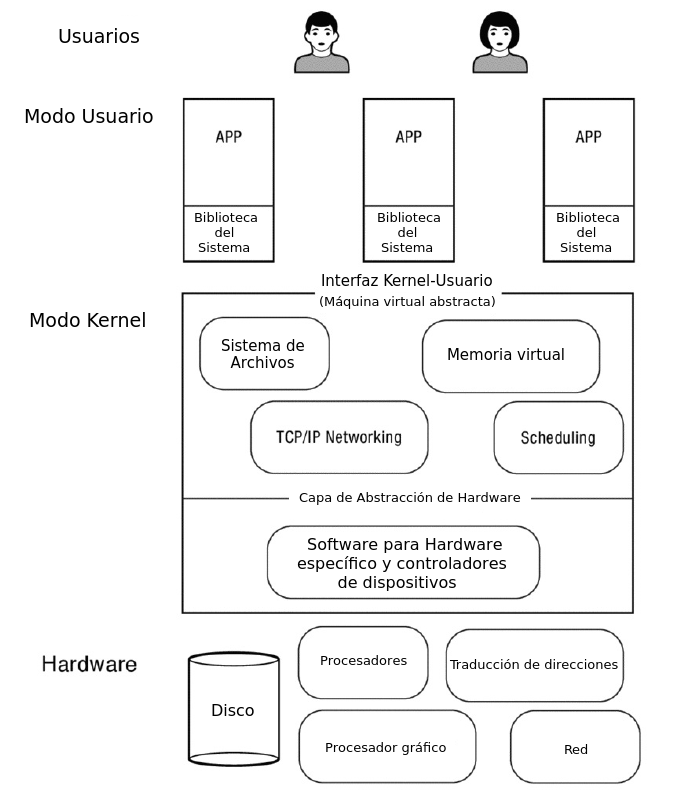
\includegraphics[scale=0.70]{img/fig0101}}
\caption{Sistema operativo de propósito general.}
\label{fig0101}
\end{figure}

Para sistemas de propósito general, los usuarios interactúan con aplicaciones, las aplicaciones se ejecutan en un entorno provisto por el sistema operativo y el sistema operativo media el acceso al hardware subyacente, como puede verse en la Figura \ref{fig0101}.

Para poder correr múltiples aplicaciones, el sistema operativo necesita desempeñar tres papeles:
\begin{enumerate}
\item \textbf{Arbitro} (\textit{Referee}). Los sistemas operativos administran los recursos compartidos entre diferentes aplicaciones ejecutándose en la misma máquina física. Por ejemplo, un sistema operativo
	\begin{itemize}
	\item Puede detener un programa e iniciar uno nuevo.
	\item Puede aislar aplicaciones entre sí, de forma que un error en una aplicación no corrompa otras aplicaciones ejecutándose en la misma máquina.
	\item Debe protegerse a sí mismo y a otras aplicaciones de virus de computadora maliciosos.
	\item Necesita decidir qué aplicaciones obtienen cuáles recursos y cuándo, dado que todas ellas comparten los recursos físicos de la computadora. 
	\end{itemize}
	
\item \textbf{Ilusionista}. Los sistemas operativos proveen una abstracción del hardware para facilitar el diseño de aplicaciones. Para escribir un programa en principio no se requeriría inferir sobre cuánta memoria física tiene el sistema o cuántos programas podrían estar compartiendo los recursos de la computadora. En cambio, los sistemas operativos proporcionan la ilusión de tener memoria casi ilimitada, a pesar de tener sólo una cantidad limitada de la misma. De la misma manera proporcionan la ilusión de que cada programa tiene todos los procesadores de la computadora para sí. Estas ilusiones permiten escribir programas independientemente de la cantidad de memoria física del sistema o de la cantidad física de procesadores. Dado que las aplicaciones son escritas a un nivel mayor de abstracción, el sistema operativo puede, casi de forma invisible, cambiar la cantidad de recursos asignados a cada aplicación.

\item \textbf{Pegamento}. Los sistemas operativos proporcionan un conjunto de servicios comunes que facilitan el intercambio de información entre aplicaciones. Como resultado de ello, \textit{cortar y pegar} funciona de manera uniforme en todo el sistema; un archivo escrito por una aplicación puede ser leído por otra. Muchos sistemas operativos proporcionan rutinas de interfaz de usuario comunes de modo que las aplicaciones pueden tener el mismo ``\textit{look and feel}''. Tal vez lo más importante, los sistemas operativos proporcionan una capa de separación de hardware de entrada/ salida (I/O) de aplicaciones, de forma que estas últimas puedan escribirse de forma independiente del teclado, el ratón y la unidad de disco específicos en uso en un equipo determinado.
\end{enumerate}

\subsection{Recursos compartidos: el Sistema Operativo como Árbitro}
La administración de recursos compartidos es un tema central del uso de la mayoría de los sistemas operativos. Un usuario podría estar corriendo al mismo tiempo un navegador web, un reproductor multimedia y un procesador de texto, entre otros. El sistema operativo debe de alguna forma mantener estas actividades separadas y a su vez permitirle a cada una el uso de toda la capacidad de la máquina si las demás no se están ejecutando. Como mínimo, cuando un programa deja de ejecutarse el sistema operativo debiese permitir ejecutar otro programa. Mejor aún, el sistema operativo debiese poder permitir la ejecución al mismo tiempo de múltiples aplicaciones. El sistema operativo es un ejemplo de software desarrollado para realizar múltiples tareas a la vez.

Compartir recursos representa las siguientes ocupaciones al sistema operativo:
\begin{itemize}
\item \textbf{Asignación de recursos}. El sistema operativo debe mantener separadas todas las actividades simultáneas, asignándole a cada una de ellas recursos de manera apropiada. Una computadora usualmente dispone de unos pocos procesadores y una cantidad limitada de memoria, ancho de banda de red y espacio en disco. Al haber varias aplicaciones ejecutándose al mismo tiempo el sistema operativo debe decidir cuántos recursos entrega a cada una. No es una tarea trivial ya que, por ejemplo, si asigna muy poca memoria a una aplicación no sólo disminuirá el rendimiento de ésta, sino también el rendimiento general de otras aplicaciones.

\item \textbf{Aislamiento}. Un error en una aplicación no debiese interrumpir la ejecución de otras aplicaciones o del sistema operativo mismo. Esto se llama \textbf{aislamiento de fallas}, el cual requiere restringir el comportamiento de las aplicaciones a menos que la plena potencia del hardware subyacente. De otra forma cualquier aplicación descargada de la web, o cualquier scrpit embebido en una página web podría controlar completamente la máquina. Cualquier aplicación podría instalar \textit{spyware} en el sistema operativo para registrar cualquier pulsación de teclas hecha por el usuario o guardar la contraseña de cada sitio web visitado. Sin el aislamiento de fallas provisto por el sistema operativo, cualquier error en un programa podría corromper irremediablemente el disco.

\item \textbf{Comunicación}. La otra cara de aislamiento es la necesidad de comunicación entre las diferentes aplicaciones y diferentes usuarios. Por ejemplo, un sitio web puede ser implementado por un conjunto de aplicaciones que cooperan entre sí: una para seleccionar los anuncios publicitarios, otra para almacenar en caché los resultados recientes, otra para traer y combinar datos desde el disco, etc. Para que esto funcione, los diversos programas deben comunicarse entre sí. Si el sistema operativo impide que los errores y aplicaciones y usuarios maliciosos afecten a otros usuarios y sus aplicaciones, entonces ¿cómo hace también para soportar la comunicación y compartir los resultados? Al crear límites, un sistema operativo también debe permitir que esos límites puedan cruzarse con cuidado en maneras controladas cuando surja la necesidad.
\end{itemize}


\subsection{Limitaciones del enmascaramiento: el Sistema Operativo como Ilusionista}
Una segunda función importante de un sistema operativo es enmascarar las restricciones inherentes al hardware del ordenador. Las restricciones físicas limitan los recursos de hardware -- un ordenador tiene sólo un número limitado de procesadores y una cantidad limitada de memoria física, el ancho de banda de red y disco --. Además, como el sistema operativo debe decidir cómo dividir sus recursos fijos entre las diferentes aplicaciones
funcionando a cada momento, una aplicación particular puede tener diferentes cantidades de recursos cada cierto tiempo, incluso cuando se ejecutan en el mismo hardware.

La \textbf{virtualización} ofrece a una aplicación la ilusión de recursos que no están físicamente presentes. Por ejemplo, el sistema operativo puede proporcionar la abstracción que cada aplicación tiene un procesador dedicado, a pesar de que a nivel físico puede haber sólo un único procesador compartido entre todas las aplicaciones que se ejecutan en el equipo.

La mayoría de los recursos físicos pueden ser virtualizados. Por ejemplo, el hardware proporciona sólo una pequeña cantidad, finita, de memoria, mientras que el sistema operativo ofrece a las aplicaciones la ilusión de una cantidad casi infinita de memoria virtual. Las redes inalámbricas eliminan paquetes corruptos; el sistema operativo enmascara estas fallas para proporcionar la ilusión de un servicio confiable.

Algunos sistemas operativos virtualizan todo el equipo, ejecutando el sistema operativo como una aplicación en encima de otro sistema operativo. Esto se conoce como crear una \textbf{máquina virtual}. El sistema operativo que se ejecuta en la máquina virtual, llamado el sistema operativo huésped, piensa que se está ejecutando en una máquina real, física, pero esto es una ilusión presentada por el verdadero sistema operativo que se ejecuta por debajo. Uno de los beneficios de una máquina virtual es la portabilidad de aplicaciones. Si un programa se ejecuta sólo en una versión antigua de un sistema operativo, aún puede trabajar en un nuevo sistema que ejecuta una máquina virtual.


\subsection{Proporcionando servicios en común: el Sistema Operativo como Pegamento}
Los sistemas operativos desempeñan un tercer papel fundamental: proporcionar un conjunto de servicios comunes, estándar a las aplicaciones para simplificar y estandarizar su diseño. Un ejemplo es el servidor web descrito anteriormente. El sistema operativo oculta los detalles de cómo funcionan los dispositivos de red y de disco, proporcionando una abstracción más simple basado en la recepción/envío de flujos fiables de bytes y la lectura/escritura de archivos con nombre. Esto le permite al servidor web enfocarse en su tarea principal --decodificar las peticiones entrantes y completarlas-- en lugar de formatear paquetes individuales la red y bloques de disco.

Una razón importante para el sistema operativo para proporcionar servicios comunes, en lugar de dejar que cada aplicación proporcionar los suyos, es facilitar el intercambio entre a las aplicaciones.


La mayoría de los sistemas operativos también ofrecen una forma estándar a las aplicaciones para pasar mensajes y compartir la memoria.


\section{Evaluación del Sistema Operativo}

\subsection{Confiabilidad y Disponibilidad}
Tal vez la característica más importante de un sistema operativo es su confiabilidad. \textbf{Confiabilidad} significa que un sistema hace exactamente lo que está diseñado para hacer. En el nivel más bajo de software ejecutándose en el sistema, los errores del sistema operativo pueden tener efectos devastadores y ocultos. Si se rompe el sistema operativo, es posible que no pueda realizar su trabajo y, en algunos casos, puede incluso perderse el trabajo previo, por ejemplo, si el fallo daña los archivos en el disco. Por el contrario, los errores de aplicación pueden ser mucho más benignos, precisamente porque los sistemas operativos proporcionan el aislamiento de fallas y un reinicio rápido y limpio después de un error.

Hacer que un sistema operativo sea confiable es un reto. Los sistemas operativos a menudo operan en un entorno hostil, donde virus y otros códigos maliciosos tratan de tomar el control del sistema explotando errores de diseño o implementación de las defensas del sistema operativo.

La \textbf{disponibilidad} es el porcentaje de tiempo que el sistema es utilizable. Un sistema operativo con errores que frecuentemente se daña, perdiendo el trabajo del usuario, es a la vez no confiable y no disponible. Un sistema operativo con errores que frecuentemente se daña, pero nunca pierde el trabajo del usuario y no puede ser alterado por un ataque malicioso es confiable pero no disponible. Un sistema operativo que ha sido alterado pero aparenta seguir funcionando con normalidad no es confiable, pero está disponible.

De este modo, tanto la confiabilidad como la disponibilidad son deseables. La disponibilidad es afectada por dos factores: la frecuencia de fallos, medido como el tiempo medio hasta el fallo (MTTF: \textit{Mean Time To Failure}), y el tiempo que se necesita para restaurar un sistema a un estado de funcionamiento después de un fallo (por ejemplo, para reiniciar), llamado tiempo medio de reparación (MTTR: \textit{Mean Time To Repair}). La disponibilidad se puede mejorar mediante el aumento de la MTTF o reducir el MTTR.

\subsection{Seguridad}
Dos conceptos estrechamente relacionados con la confiabilidad son la seguridad y la privacidad. \textbf{Seguridad} significa que la operatoria del ordenador no puede ser comprometida por un atacante malintencionado. La \textbf{Privacidad} es un aspecto de la seguridad: los datos almacenados en el ordenador son sólo accesibles por usuarios autorizados.

Por desgracia, ningún ordenador útil es perfectamente seguro. Cualquier pieza compleja de software tiene errores, y los errores, en apariencia inocuos, pueden ser explotados por un atacante para obtener el control del sistema. O el hardware del ordenador puede ser manipulado, para proporcionar acceso al atacante. O el administrador del equipo podría ser poco fiable, utilizando sus credenciales para robar datos del usuario, etc.

Sin embargo, un sistema operativo puede ser, y debe ser, diseñado para minimizar su vulnerabilidad a los ataques. Por ejemplo, un fuerte aislamiento de fallos puede impedir que las aplicaciones de terceros tomen el control del sistema. Un \textbf{virus de computadora} es un programa de ordenador que modifica un sistema operativo o aplicación para copiarse a sí mismo desde un ordenador a otro sin el permiso o el conocimiento del propietario del ordenador. Una vez instalado en un ordenador, un virus a menudo proporciona el atacante el control de los recursos o los datos del sistema. Un ejemplo de virus informático es un \textit{keylogger}: un programa que modifica el sistema operativo para registrar cada pulsación de tecla introducida por el usuario y enviarlos de vuelta a la máquina del atacante. De esta manera, el atacante podría obtener acceso a las contraseñas del usuario, números de cuentas bancarias, y otra información privada.

Incluso con un fuerte aislamiento de fallos, un sistema puede ser inseguro si sus aplicaciones no están diseñadas para la seguridad. Por ejemplo un mensaje de correo electrónico puede parecer de alguien (tal vez alguien de confianza), cuando en realidad se trata del atacante y contiene, como un archivo adjunto, un virus malicioso.

Para complicar aún más las cosas, el sistema operativo no sólo debe impedir el acceso no autorizado a los datos compartidos, sino que también debe permitir el acceso en muchos casos. Los usuarios y los programas deben ser capaces de interactuar entre sí, de modo que es posible cortar y pegar texto entre diferentes aplicaciones, y para compartir los datos escritos en el disco o en la red.

Por lo tanto, un sistema operativo necesita tanto un mecanismo de aplicación y de una política de seguridad. Un \textbf{mecanismo de aplicación} es la forma en que el sistema operativo se asegura de que sólo se realicen acciones permitidas. La \textbf{política de seguridad} define lo que está permitido: quién está autorizado a acceder a qué datos, y quién puede realizar qué tipo de operaciones.

\subsection{Portabilidad}
Todos los sistemas operativos proporcionan aplicaciones con una abstracción del hardware subyacente; una abstracción portable es una que no cambia con cambios en el hardware. Un programa escrito para Microsoft Windows debería funcionar correctamente, independientemente de si se está utilizando una tarjeta gráfica específica, si el almacenamiento persistente se proporciona a través de la memoria flash o disco magnético rotatorio, o si la red es Bluetooth, Wi-Fi o Ethernet Gigabit.

La portabilidad también se aplica al propio sistema operativo. Es poco práctico reescribir sistemas operativos desde cero cada vez que se desarrolla un nuevo hardware o una nueva aplicación. En cambio, los nuevos sistemas operativos a menudo se derivan, al menos en parte, a partir de los antiguos. Como resultado, la mayoría de los sistemas operativos de éxito tienen un tiempo de vida medido en décadas. Esto significa que los sistemas operativos deben ser diseñados para soportar aplicaciones que aún no se han escrito y para ejecutarse en hardware que aún no ha sido desarrollado. Del mismo modo, los desarrolladores no quieren volver a escribir las aplicaciones cuando el sistema operativo es portado de una máquina a otra.

En el diseño de un sistema operativo para lograr la portabilidad, es de ayuda tener una forma simple y estándar para que  las aplicaciones interactúen con el sistema operativo. Una \textbf{máquina virtual abstracta} (AVM: \textit{Abstract Virtual Machine}) es la interfaz proporcionada por los sistemas a aplicaciones, incluyendo la operación de:
\begin{enumerate}
\item La interfaz de programación de aplicaciones (API: \textit{Application Programming Interface}) que es la lista de llamadas a funciones del sistema operativo proporcionada a las aplicaciones.
\item El modelo de acceso a la memoria.
\item El tipo y cantidad de instrucciones que pueden ser ejecutadas legalmente.
\end{enumerate}

Una AVM de un sistema operativo bien diseñada ofrece un punto fijo a través del cual tanto el código de aplicación y hardware pueden evolucionar de forma independiente. Esto es similar a la función del protocolo de Internet (IP) estándar en redes. Las aplicaciones distribuidas como el correo electrónico y la Web, escrita usando IP, están aislados de los cambios en la tecnología de red subyacente (Ethernet, Wi-Fi, etc.). Es igualmente importante que los cambios en las aplicaciones, desde el correo electrónico, la mensajería instantánea o el intercambio de ficheros, no requieran cambios simultáneos en el hardware subyacente.

El sistema operativo en sí mismo en gran medida se puede implementar de forma independiente de los detalles específicos del hardware. La interfaz que hace que esto sea posible se llama la capa de abstracción de hardware (HAL: \textit{Hardware Abstraction Layer}). Podría parecer que la AVM y la  HAL del sistema operativo son idénticas dado que ambas son capas portables diseñadas para ocultar los detalles de hardware. Sin embargo la AVM debe hacer más. Las aplicaciones se ejecutan en un contexto restringido, virtualizado y con acceso a servicios comunes de alto nivel, mientras que el propio sistema operativo utiliza una abstracción de procedimientos mucho más cercana al hardware real.

\subsection{Rendimiento}
Mientras que la portabilidad de un sistema operativo se hace evidente con el tiempo, el rendimiento de un sistema operativo es a menudo inmediatamente visible a sus usuarios. A pesar de que el rendimiento con frecuencia se asocia a cada aplicación individual, el diseño del sistema operativo puede afectar en gran medida el rendimiento percibido de la aplicación. El sistema operativo decide cuándo una aplicación se puede ejecutar, la cantidad de memoria que puede utilizar, y si sus archivos se almacenan en la memoria caché o agrupados de manera eficiente en el disco. Los sistemas operativos también median el acceso de las aplicaciones a la memoria, la red, y el disco. Debe evitar la ralentización de la ruta crítica, mientras que todavía proporciona el aislamiento de fallos necesario y el intercambio de recursos entre aplicaciones.

El rendimiento no es una sola cantidad. Más bien, se puede medir de varias maneras diferentes. 
\begin{itemize}
\item \textbf{Sobrecarga} (\textit{overhead}): es el costo de los recursos añadido a la implementación de una abstracción presentada a las aplicaciones. 
\item \textbf{Eficiencia}: es la falta de sobrecarga en una abstracción.

Una manera de medir la sobrecarga (o inversamente, la eficiencia) es el grado en que la abstracción impide rendimiento de la aplicación. Supongamos que se podría ejecutar la aplicación directamente en el hardware subyacente, sin la sobrecarga de la abstracción del sistema operativo: ¿cuánto mejoraría el rendimiento de la aplicación?

\item \textbf{Equidad}: es la manera de dividir los recursos de forma equitativa entre los diferentes usuarios o aplicaciones que se ejecutan en la misma máquina. Esto plantea interrogantes a cómo debe decidir el sistema operativo si los recursos tienen que ser divididos en partes iguales entre los diferentes usuarios o aplicaciones, o si alguno de ellos debe percibir un trato preferencial.

\item \textbf{Tiempo de respuesta}: a veces llamado retardo, es el tiempo que tarda una sola tarea en ejecutarse, desde el momento en que comienza hasta que se completa. Por ejemplo, un tiempo de respuesta muy visible para ordenadores de escritorio es el tiempo desde que el usuario mueve el ratón hasta que el puntero en la pantalla refleja la acción del usuario. Un sistema operativo que proporciona tiempo de respuesta pobre puede ser inutilizable.

\item \textbf{Volumen de trabajo (throughput)}: es la velocidad a la que el sistema completa tareas. El throughput es una medida de la eficiencia para un grupo de tareas en lugar de una sola. Aunque podría parecer que los diseños que mejoran el tiempo de respuesta también lo hacen con el throughput, este no es el caso.

\item \textbf{Previsibilidad de rendimiento}: indica si el tiempo de respuesta del sistema u otra métrica es constante en el tiempo. La previsibilidad a menudo puede ser más importante que el rendimiento promedio. Si una operación de usuario a veces toma un instante, pero a veces mucho más tiempo, el usuario puede tener dificultades para adaptarse.
\end{itemize}


\subsection{Adopción}
Además de la fiabilidad, portabilidad y rendimiento, el éxito de un sistema operativo depende de dos factores fuera de su control inmediato: la amplia disponibilidad de las aplicaciones portadas a ese sistema operativo, y la amplia disponibilidad de hardware que el sistema operativo puede soportar.

El \textbf{efecto de red} se produce cuando el valor de una tecnología no sólo depende de sus capacidades intrínsecas, sino también en el número de otras personas que lo han adoptado. Los diseñadores de aplicaciones y hardware invierten sus esfuerzos en las plataformas de sistemas operativos con la mayor cantidad de usuarios, mientras que los usuarios prefieren los sistemas operativos con las mejores aplicaciones o el hardware más barato. Más usuarios implican más aplicaciones y el hardware más barato; más aplicaciones y el hardware más barato implican a más usuarios, en un círculo virtuoso.

Un \textbf{sistema propietario} es uno bajo el control de una única empresa; puede ser cambiado en cualquier momento por su proveedor para satisfacer las necesidades de sus clientes. Un \textbf{sistema abierto} es aquel donde el código fuente del sistema es público, dando a cualquier persona la posibilidad de inspeccionar y cambiar el código. A menudo, un sistema abierto tiene una API que se puede cambiar con el acuerdo de un organismo público de normalización. La adhesión a las normas garantiza a los desarrolladores de aplicaciones que la API no será cambiada, excepto por acuerdo general. Por otra parte, los organismos de normalización pueden hacer que sea difícil para agregar rápidamente nuevas características solicitadas o requeridas. 

Ninguno de los dos sistemas, abiertos ni propietarias, son intrínsecamente mejor para su adopción. Windows y MacOS son sistemas operativos propietarios; Linux es un sistema operativo abierto. Los tres son ampliamente utilizados. Los sistemas abiertos son más fáciles de adaptar a una amplia variedad de plataformas de hardware, pero corren el riesgo de recaer en múltiples versiones, deteriorando el efecto de red. Los proveedores de sistemas operativos propietarios argumentan que sus sistemas son más fiables y mejor adaptado a las necesidades de sus clientes. Los problemas de interoperabilidad pueden ser reducidos si la misma empresa controla tanto el hardware como el software, pero la limitación de un sistema operativo a una plataforma de hardware perjudica el efecto de red y podría alejar a los consumidores.

\subsection{Compromisos de Diseño}
La mayoría de los diseños prácticos de sistemas operativos establecen un equilibrio entre los objetivos de confiabilidad, seguridad, portabilidad, rendimiento y adopción. Las opciones de diseño que mejoran la portabilidad -- por ejemplo, la preservación de las interfaces heredadas -- a menudo hacen que el sistema sea en su conjunto menos confiable y menos seguro. Del mismo modo, a menudo es posible aumentar el rendimiento del sistema mediante la ruptura de una abstracción. Sin embargo, este tipo de optimizaciones de rendimiento pueden añadir complejidad y, por lo tanto, potencialmente dañar la confiabilidad. El diseñador del sistema operativo debe sopesar cuidadosamente estos objetivos en conflicto.


\section{Sistemas Operativos: Pasado, Presente y Futuro}
Como la capa más baja de software que se ejecuta sobre el hardware de equipos informáticos, los sistemas operativos se remontan a los primeros ordenadores, evolucionando casi tan rápidamente como el hardware.

\subsection{Impacto de las tendencias tecnológicas}
El aspecto más sorprendente de los últimos cincuenta años en la tecnología informática ha sido el efecto acumulativo de la Ley de Moore y los avances comparables en las tecnologías relacionadas, como la memoria y almacenamiento en disco. La \textbf{Ley de Moore} establece que la densidad de transistores aumenta exponencialmente con el tiempo; mejoras exponenciales similares han ocurrido en muchas otras tecnologías de componentes.

Desde 1981 a la actualidad el costo de procesamiento y la memoria se ha reducido en casi seis órdenes de magnitud; el costo de la capacidad del disco se ha reducido en siete órdenes de magnitud. No todas las tecnologías han mejorado en la misma proporción; la latencia de discoha mejorado, pero a un ritmo mucho más lento que la capacidad del disco. Estos cambios relativos han alterado radicalmente tanto el uso de las computadoras y las ventajas y desventajas que enfrentan los diseñadores de sistemas operativos.

En los primeros años de la informática, los ordenadores eran más caros que los salarios de las personas que los utilizan. Los usuarios hacían cola esperando su turno para ejecutar un programa. Con el tiempo, las computadoras se han vuelto lo suficientemente baratas como para permanecer inactivas hasta que las necesitemos.

A pesar de estos cambios, los sistemas operativos todavía se enfrentan a los mismos retos conceptuales como lo hicieron hace cincuenta años. Para gestionar los recursos informáticos para aplicaciones y usuarios, se deben asignar los recursos entre aplicaciones, proporcionar aislamiento de fallos y servicios de comunicación, proveer limitaciones abstractas de hardware, etc. Aunque no se sabe con precisión cómo la tecnología informática o la demanda de aplicaciones van a evolucionar, es muy probable que persistan estos retos fundamentales de los sistemas operativos.

\subsection{Primeros Sistemas Operativos}
Los primeros sistemas operativos eran bibliotecas de ejecución destinadas a simplificar la programación de los primeros sistemas informáticos. Los primeros ordenadores a menudo ocupaban toda una planta de un depósito, costaban millones de dólares, y sin embargo, eran capaces de ser utilizados sólo por una persona a la vez. El usuario primero restablecía el sistema, cargaba el programa conmutando en el sistema de un solo bit a la vez, y pulsaba '\textit{go}', produciendo la salida para ser estudiada minuciosamente durante el turno del siguiente usuario. Si el programa tenía un error, el usuario tendría que esperar a probar la ejecución otra vez.

Los primeros sistemas operativos se desarrollaron como una forma de reducir los errores al proporcionar un conjunto estándar de servicios comunes. Por ejemplo, los primeros sistemas operativos proporcionaban rutinas estándar de entrada/salida (E/S) que cada usuario podía vincular a sus programas. Estos servicios hacían que fuera más probable que el programa de un usuario produjera una salida útil.

\subsection{Sistemas Operativos Multi-Usuario}
El siguiente paso fue compartir. Cuando el tiempo de procesador es valioso, restringiendo el sistema a un usuario a la vez es un desperdicio. Por ejemplo, en los primeros sistemas el procesador quedaba inactivo mientras el usuario cargaba el programa. Un \textbf{sistema operativo por lotes (batch)} funciona con una cola de tareas. Se ejecuta un bucle simple: cargar, ejecutar, y descargar cada trabajo por vez. Mientras que un trabajo ya está en marcha, el sistema operativo configura los dispositivos de E/S para hacer transferencias de fondo para el trabajo siguiente/anterior mediante un proceso denominado acceso directo a memoria (DMA: \textit{Direct Memory Access}). Con DMA, el dispositivo de E/S transfiere sus datos directamente a la memoria en un lugar especificado por el sistema operativo. Cuando la transferencia de E/S se completa, el hardware interrumpe el procesador, transfiriendo el control al manejador de interrupciones del sistema operativo. El sistema operativo inicia la siguiente transferencia de DMA y luego continúa con la ejecución de la aplicación. La interrupción se muestra a la aplicación como si no hubiera pasado nada, salvo algún retraso entre una instrucción y la siguiente.

Los sistemas operativos por lotes pronto se extendieron para ejecutar varias aplicaciones a la vez. Esto se llamó \textbf{multitarea} o, a veces \textbf{multiprogramación}. Múltiples programas se cargan en la memoria al mismo tiempo, cada uno listo para usar el procesador si por cualquier razón la tarea anterior necesita hacer una pausa, por ejemplo, para leer la entrada adicional o producir de salida. La multitarea aumenta la eficiencia del procesador a casi el 100 \%. Sin embargo, el uso compartido de procesador plantea la necesidad de aislamiento de programas, para evitar que un error en un programa dañe o corrompa otro. Durante este período, los diseñadores de computadoras añaden protección de memoria de hardware, para reducir la sobrecarga (overhead) del aislamiento de fallos.

Un desafío práctico con la computación por lotes, sin embargo, es cómo depurar el sistema operativo en sí mismo. A diferencia de un programa de aplicación, un sistema operativo por lotes asume que está en control directo del hardware. Las nuevas versiones sólo pueden ser probadas al detener todas las aplicaciones y reiniciar el sistema, esencialmente equivale a volver al esquema de ordenador con un sistema operativo de un solo usuario.


\subsection{Sistemas Operativos de Tiempo Compartido}
Con el tiempo, el efecto acumulativo de la Ley de Moore significó que el coste de la computación se redujera al punto donde los sistemas podrían ser optimizados para los usuarios en lugar de para un uso eficiente del procesador. UNIX, por ejemplo, se convirtió en la base para de Apple MacOS X, Linux y Android de Google, entre otros.

Los \textbf{sistemas operativos de tiempo compartido} -- como Windows, MacOS o Linux -- están diseñados para soportar el uso interactivo de la computadora en lugar del procesamiento por lotes de los sistemas anteriores. Con el tiempo compartido, la entrada es suministrada por un usuario mientras escribe en un teclado o utiliza otro dispositivo de entrada conectado directamente al ordenador. Cada pulsación de tecla o acción del ratón provoca una interrupción indicándole un evento al procesador; el controlador de interrupciones lee el evento desde el dispositivo y lo pone en cola dentro del sistema operativo. Cuando la aplicación reanuda, se obtiene el evento desde el sistema operativo, se procesa y se modifica el display (e.g. pantalla del monitor) debidamente antes de ir a buscar el próximo evento. Cientos o incluso miles de tales eventos pueden ser procesados por segundo, lo que requiere que tanto el sistema operativo como la aplicación se diseñen para ráfagas frecuentes de muy corta actividad en vez del modelo de ejecución sostenida del procesamiento por lotes.

Los primeros sistemas de tiempo compartido permitieron tener muchos usuarios en simultáneo, pero incluso esto fue sólo una fase. Con el tiempo, las computadoras se volvieron lo suficientemente baratas como para que las personas pudieran permitirse sus propios ordenadores ``personales'' dedicados. El acceso a los datos compartidos se convirtió en primordial, consolidando el cambio a la computación cliente-servidor.


\subsection{Sistemas Operativos Modernos}
Hoy en día, existe una gran diversidad de dispositivos de cómputo, con diferentes sistemas operativos que se ejecutan en ellos. Las ventajas y desventajas que enfrenta un diseñador de sistemas operativos dependen de las capacidades físicas del hardware, así como las necesidades de aplicación y de usuario. Los siguientes son algunos ejemplos de sistemas operativos modernos.

\begin{itemize}
\item \textbf{Sistemas Operativos de Escritorio, Laptop y Netbook}

Ejemplos incluyen Windows, MacOS y Linux. Estos sistemas son de un solo usuario, ejecutan muchas aplicaciones y tienen varios dispositivos de E/S. Los sistemas operativos iniciales para PCs tenían una capacidad muy limitada para aislar diferentes partes del sistema de las demás. Con el tiempo, sin embargo, se hizo evidente que se necesitaba un aislamiento de fallos más estricto para mejorar la confiabilidad del sistema y la resistencia contra los virus informáticos. Otros objetivos clave de diseño para estos sistemas incluyen la adopción (para apoyar un amplio conjunto de aplicaciones) y el rendimiento interactivo.

\item \textbf{Sistemas Operativos para \textit{Smartphones}}

Un \textit{smartphone} es un teléfono móvil con un ordenador incorporado capaz de ejecutar aplicaciones de terceros. Ejemplos de sistemas operativos de \textit{smartphones} incluyen iOS, Android y Windows Phone. Los teléfonos inteligentes tienen sólo un usuario, pero deben ser compatibles con muchas aplicaciones. Objetivos clave de diseño incluyen la capacidad de respuesta, el soporte a una amplia variedad de aplicaciones, y el uso eficiente de la batería. Otro objetivo de diseño es la privacidad del usuario. Debido a que las aplicaciones de terceros pueden recopilar datos privados sigilosamente con fines de comercialización, como la lista de contactos del usuario, el sistema operativo debe estar diseñado para limitar el acceso a los datos protegidos del usuario.

\item \textbf{Sistemas Operativos para Servidores}

Los motores de búsqueda, medios de comunicación web, sitios de comercio electrónico, y sistemas de correo electrónico están alojados en los equipos de los centros de datos; cada uno de estos ordenadores ejecuta un sistema operativo, a menudo una versión de potencia industrial de uno de los sistemas de escritorio descritos anteriormente. Por lo general, sólo una única aplicación, como un servidor web, se ejecuta por máquina, pero el sistema operativo debe coordinar miles de conexiones de red entrantes simultáneas. El rendimiento en el manejo de un gran número de solicitudes por segundo es un objetivo clave de diseño. Al mismo tiempo, hay una bonus en la capacidad de respuesta. Los servidores también operan en un ambiente hostil, donde los atacantes maliciosos pueden intentar alterar o bloquear el servicio; la resistencia al ataque es un requisito esencial.

\item \textbf{Máquinas Virtuales}

Un monitor de máquina virtual es un sistema operativo que puede ejecutar otro sistema operativo como si se tratara de una aplicación. Los ejemplos incluyen VMware, Xen y Windows Virtual PC. Los monitores de máquinas virtuales enfrentan muchos de los mismos problemas que otros sistemas operativos, con el reto añadido que supone la coordinación de un conjunto de coordinadores. Un sistema operativo huésped en ejecución en una máquina virtual toma decisiones de asignación de recursos y de aislamiento de fallas como si estuviera en completo control de sus recursos, a pesar de que está compartiendo el sistema con otros sistemas operativos y aplicaciones.

\item \textbf{Sistemas Embebidos}

Con el tiempo, las computadoras se han vuelto lo suficientemente baratas para integrarse a cualquier número de dispositivos de consumo, desde decodificadores de televisión por cable a sistemas de control para automóviles y aviones. Los dispositivos embebidos suelen ejecutar un sistema operativo personalizado incluido con software específico para las tareas que controla el dispositivo. Merecen mucha atención, ya que los errores de software en ellos pueden tener efectos devastadores.

\item \textbf{Clústeres de Servidores}

Para tolerancia a fallos, escala y capacidad de respuesta, los sitios web se implementan cada vez más en clústeres de ordenadores alojados en uno o más centros de datos distribuidos geográficamente en ubicaciones cercanas a los usuarios. Si un equipo falla debido a un desperfecto de hardware, error de software o interrupción en la alimentación, otro equipo puede hacerse cargo de su función. Si la demanda para el sitio Web supera lo que un solo equipo puede manejar, las peticiones web se pueden dividir entre varias máquinas. Al igual que con los sistemas operativos normales, las aplicaciones de clústeres de servidores se ejecutan en la parte superior de una interfaz de clúster abstracto para aislar la aplicación de cambios de hardware y para evitar que fallos en una aplicación afecten a otras aplicaciones en el mismo centro de datos. Del mismo modo, los recursos pueden ser compartidos entre: (1) varias aplicaciones en el mismo sitio web (como Google Search, Google Earth, y Gmail), y (2) varios sitios web alojados en el mismo hardware del clúster (por ejemplo, Compute Engine de Google).
\end{itemize}


\subsection{Sistemas Operativos Futuros}
En primer lugar, dado que pueden presentarse desafíos de seguridad y confiabilidad, potenciales enormes beneficios podrían ser el resultado de tener computadoras controladas firmemente y poder coordinar la infraestructura física, como la red eléctrica, la red telefónica, y los dispositivos médicos y sistemas de registros médicos de un hospital. En segundo lugar, los cambios en el hardware subyacente a menudo desencadenan un nuevo trabajo en el diseño de sistemas operativos. El futuro de los sistemas operativos es también el futuro de hardware:

\begin{itemize}
\item Centros de cómputos a muy gran escala.
\item Sistema multi-núcleo a muy gran escala.
\item Dispositivos informáticos portátiles multi-funcionales ubicuos (portables a todas partes).
\item Sistemas muy heterogéneos (como todos los dispositivos se vuelven programables, se necesitarán sistemas operativos para una gran variedad de dispositivos, desde los superordenadores a los refrigeradores).
\item Almacenamiento a muy gran escala.
\end{itemize}

\clearpage

\chapter{La Abstracción del Kernel}
Un rol central de los sistemas operativos es la \textbf{protección} -- el aislamiento de aplicaciones y usuarios potencialmente dañinos para evitar que corrompan otras aplicaciones o el propio sistema operativo. La protección es esencial para lograr algunos de los objetivos mencionados antes:
\begin{itemize}
\item Confiabilidad
\item Seguridad
\item Privacidad
\item Asignación de recursos equitativa
\end{itemize}

La implementación de la protección es el trabajo del kernel o núcleo del sistema operativo. El \textbf{kernel}, el nivel más bajo de software que se ejecuta en el sistema, tiene acceso completo a todo el hardware de la máquina. El núcleo es de confianza, necesariamente para poder hacer cualquier cosa con el hardware. El resto -- es decir, el software que se ejecuta en el sistema que no es de confianza -- se ejecuta en un entorno restringido con menos que el completo acceso a toda la potencia del hardware.

Por su parte, las aplicaciones en sí a menudo necesitan ejecutar código no confiable de terceros de manera segura. Un ejemplo es un navegador web que ejecuta código \textit{JavaScript} integrado para elaborar una página web. Sin protección, un \textit{script} con un virus incrustado puede tomar el control del navegador, por lo que los usuarios piensan que están interactuando directamente con la web, cuando en realidad sus contraseñas web podrían estar siendo desviadas a un atacante.

Un \textbf{proceso} es la ejecución de un programa de aplicación con derechos restringidos; el proceso es la abstracción de ejecución protegida proporcionada por el kernel del sistema operativo. Un proceso necesita el permiso del kernel del sistema operativo antes de acceder a la memoria de cualquier otro proceso, antes de leer o escribir en el disco, antes de cambiar la configuración de hardware, y así sucesivamente. En otras palabras, el kernel del sistema operativo arbitra y controla el acceso de cada proceso al hardware.

El kernel del sistema operativo se ejecuta directamente en el procesador con derechos ilimitados. El kernel puede realizar cualquier operación disponible en el hardware. Las aplicaciones necesitan ejecutarse en el procesador con todas las operaciones potencialmente peligrosas deshabilitadas. Para que esto funcione, el hardware necesita proporcionar un poco de ayuda. Tanto el kernel del sistema operativo como los procesos de las aplicaciones --que se ejecutan con derechos restringidos-- comparten la misma máquina: el mismo procesador, la misma memoria y el mismo disco.


\section{La Abstracción del Proceso}
Un programador escribe código en un lenguaje de alto nivel. Un compilador convierte el código en una secuencia de instrucciones de máquina y almacena esas instrucciones en un archivo, llamado \textbf{imagen ejecutable} del programa. El compilador también define los datos estáticos que el programa necesita, junto con sus valores iniciales, y los incluye en la imagen ejecutable.

Para ejecutar el programa, el sistema operativo copia las instrucciones y los datos de la imagen ejecutable en la memoria física. El sistema operativo deja de lado una región de memoria, la \textbf{pila de ejecución}, para mantener el estado de las variables locales durante las llamadas de procedimiento. El sistema operativo también deja de lado una región de memoria, llamada \textbf{heap}, para cualquier estructura de datos asignada dinámicamente que podría necesitar el programa. Por supuesto, para copiar el programa en la memoria, el sistema operativo mismo debe estar ya cargado en la memoria, con su propia pila y \textit{heap}. Ignorando la protección, una vez que un programa se carga en memoria, el sistema operativo puede iniciarlo ajustando el puntero de pila y el salto a la primera instrucción de programa. El propio compilador es un programa más: el sistema operativo inicia el compilador insertando su imagen ejecutable en la memoria y saltando a su primera instrucción.


Para ejecutar varias copias del mismo programa, el sistema operativo puede hacer múltiples copias de las instrucciones del programa, datos estáticos, \textit{heap} y la pila en la memoria. La mayoría de los sistemas operativos reutilizan la memoria siempre que sea posible: almacenan sólo una única copia de las instrucciones de un programa cuando múltiples copias del programa se ejecutan al mismo tiempo. A pesar de ello, se necesita una copia separada de los datos del programa, \textit{heap} y pila.

Por lo tanto, un proceso es un ejemplo de un programa, de la misma manera que un objeto es una instancia de una clase en la programación orientada a objetos. Cada programa puede tener cero, uno o más procesos en ejecución Para cada instancia de un programa, hay un proceso con su propia copia del programa en la memoria.

El sistema operativo lleva un registro de los diversos procesos en el equipo utilizando una estructura de datos llamada bloque de control de proceso, o PCB (\textit{Process Control Block}). Los PCB almacenan toda la información que el sistema operativo necesita acerca de un proceso en particular: dónde se almacena en la memoria, en qué parte del disco reside su imagen ejecutable, qué usuario solicitó ejecutarlo, qué privilegios tiene el proceso, etc.

Algunos programas se componen de múltiples actividades simultáneas, o hilos. Un navegador web, por ejemplo, podría necesitar recibir la entrada del usuario, al mismo tiempo que se está dibujando la pantalla o recibiendo entrada de red. Cada una de estas actividades por separado tiene su propio contador de programa y pila, pero opera en el mismo código y datos como los demás hilos. El sistema operativo ejecuta múltiples hilos en un proceso, en la misma forma que ejecuta varios procesos en la memoria física.

\textbf{Procesos, procesos ligeros e hilos}
Un hilo (\textit{thread}) es una secuencia lógica de instrucciones que ejecutan tanto el sistema operativo como los códigos de aplicación. Un programa multiprocesador puede tener varias secuencias de instrucciones que se ejecutan en paralelo, cada uno con su propio contador de programa, pero todos cooperando dentro de un único límite de protección. Durante un tiempo, éstos fueron llamados ``procesos ligeros'' (cada uno es una secuencia de instrucciones que cooperan dentro de un límite de protección), pero con el tiempo la palabra ``hilo'' se volvió más ampliamente utilizada.

Esto conduce a la convención de nombres actualmente utilizada en casi todos los sistemas operativos modernos: \textbf{un \textit{proceso} ejecuta un \textit{programa}, que consta de uno o más \textit{hilos} que se ejecutan dentro de un \textit{límite de protección}}.


\section{El Modo Dual de Operación}
Una vez que un programa se carga en memoria y el sistema operativo inicia el proceso, el procesador trae una instrucción por vez; a continuación la decodifica y ejecuta. Algunas instrucciones calculan los valores, por ejemplo, al multiplicar dos registros y poner el resultado en otro registro. Algunas instrucciones leen o escriben ubicaciones en la memoria. Y otras instrucciones, como las ramas (saltos/\textit{branches}) o las llamadas de procedimiento, cambian el contador de programa y de este modo determinan la siguiente instrucción a ejecutar.

\begin{figure}[tbhp]
\centerline{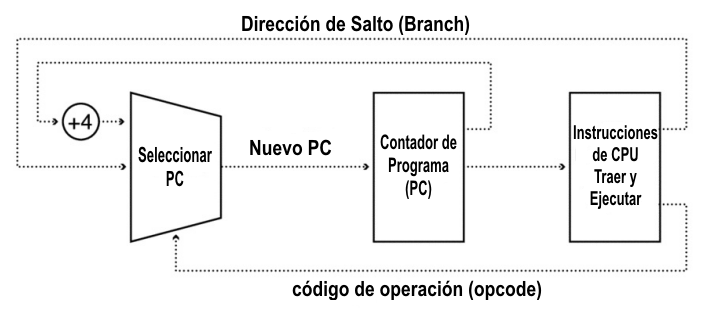
\includegraphics[scale=0.70]{img/fig0201}}
\caption{La operación básica de una CPU.}
\label{fig0201}
\end{figure}

Ahora, ¿cómo el kernel del sistema operativo evita que un proceso dañe otros procesos o el propio sistema operativo? Después de todo, cuando múltiples programas se cargan en la memoria al mismo tiempo, ¿qué impide que un proceso sobrescriba las estructuras de datos de otro proceso, o incluso sobrescriba la imagen del sistema operativo almacenado en el disco? La mayoría de las instrucciones son perfectamente seguras, tales como la adición de dos registros y almacenar el resultado en un tercer registro. ¿Se puede modificar el procesador de alguna manera para permitir que las instrucciones seguras se ejecuten directamente en el hardware? Para lograr esto, se implementa el denominado \textbf{modo dual de operación}, representado por un único bit en el registro de estado del procesador que indica el modo actual del procesador. En el \textbf{modo de usuario}, el procesador comprueba cada instrucción antes de ejecutarla para verificar que está permitida para ser realizada por ese proceso. En modo de kernel, el sistema operativo se ejecuta con los controles de protección apagados.

\textit{\textbf{El kernel vs. el resto del sistema operativo}}

El kernel es una pieza fundamental de un sistema operativo, pero es sólo una parte del sistema operativo en general. En la mayoría de los sistemas operativos modernos, una parte del mismo se ejecuta en modo de usuario como una biblioteca vinculada a cada aplicación. Un ejemplo es el código de la biblioteca que gestiona los botones de menú de una aplicación. El código de la biblioteca (pero no el kernel del sistema operativo) \textit{comparte el mismo destino} que el resto de la aplicación: un problema con uno tiene el mismo efecto que un problema con el otro.

Del mismo modo, partes del sistema operativo pueden ejecutarse en sus propios procesos a nivel de usuario. Un gestor de ventanas es un ejemplo. El gestor de ventanas dirige las acciones del ratón y la entrada de teclado que se producen dentro de una ventana a la aplicación correcta, y el administrador también se asegura de que cada aplicación modifique sólo la parte de la pantalla correspondiente a la aplicación, y no la barra de menús del sistema operativo o cualquier otra ventana de aplicación. Sin esta restricción, una aplicación maliciosa podría tomar el control de la máquina. Por ejemplo, un virus podría presentar una pantalla de login que luzca idéntica a la del sistema, lo que podría inducir a los usuarios a revelar sus contraseñas al atacante.

Otro motivo para tener separado del kernel al resto del sistema operativo (código de bibliotecas y cualquier aplicación de nivel usuario) es que a menudo es más fácil de depurar el código de nivel de usuario que el código del kernel. Más importante aún, el kernel debe ser de confianza, ya que tiene control total sobre el hardware. Cualquier error en el kernel puede corromper el disco, la memoria de otras aplicaciones, o simplemente bloquear el sistema. Al separar el código que no necesita estar en el kernel, el sistema operativo puede ser más confiable -- un error en el sistema de ventanas es bastante malo, pero sería aún peor si se podría corromper el disco. Esto ilustra el \textbf{principio de mínimo privilegio}: la seguridad y la confiabilidad aumentan si cada parte del sistema tiene exactamente los privilegios que necesita para hacer su trabajo, y nada más.

\begin{figure}[tbhp]
\centerline{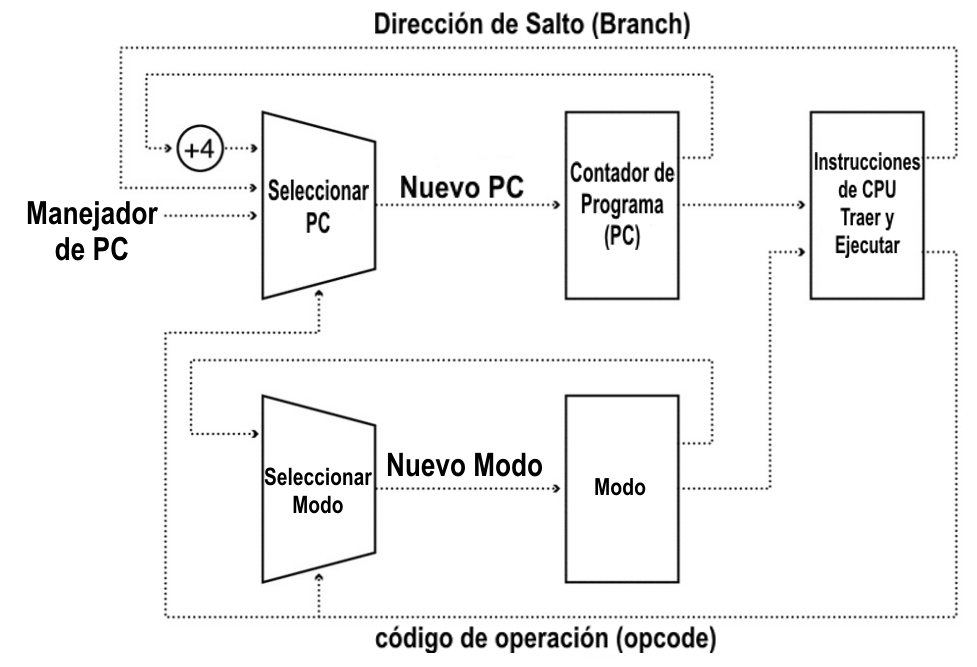
\includegraphics[scale=0.54]{img/fig0202}}
\caption{El funcionamiento de una CPU con los modos kernel y usuario.}
\label{fig0202}
\end{figure}

En la Figura \ref{fig0202} se muestra el funcionamiento de un procesador de modo dual; el contador de programa y el bit de modo juntos controlan el funcionamiento del procesador. A su vez, el bit de modo es modificado por algunas instrucciones, tal como el contador de programa es modificado por algunas instrucciones. Para permitir al kernel del sistema operativo proteger las aplicaciones y los usuarios unos de otros, pero también dejar que código de usuario se ejecute directamente en el procesador, como mínimo, el hardware debe ser compatible con tres cosas:

\begin{itemize}
\item \textbf{Instrucciones privilegiadas}: todas las instrucciones potencialmente inseguras están prohibidas cuando se ejecutan en modo usuario.
\item \textbf{Protección de memoria}: todos los accesos a memoria fuera de la región de memoria válida de un proceso están prohibidos cuando se ejecutan en modo usuario.
\item \textbf{Interrupciones del temporizador}: independientemente de lo que hace el proceso, el kernel debe tener una manera de recuperar periódicamente el control del proceso actual.
\end{itemize}

Además, el hardware también debe proporcionar una forma de transferir de forma segura de control de modo usuario a modo kernel y viceversa.


\subsection{Instrucciones Privilegiadas}
El aislamiento de procesos es posible sólo si hay una manera de limitar los programas que se ejecutan en modo usuario de cambiar directamente su nivel de privilegio. Los procesos pueden indirectamente cambiar su nivel de privilegio mediante la ejecución de una instrucción especial, denominada \textbf{llamada al sistema}, para transferir el control al kernel desde una ubicación fija definida por el sistema operativo. Aparte de la transferencia de control al kernel del sistema operativo (esto es, en efecto, convertirse en el kernel) en estas ubicaciones fijas, un proceso de aplicación no puede cambiar su nivel de privilegio.

Otras instrucciones también se limitan a ser utilizadas sólo por código del kernel. La se puede permitir a una aplicación que cambie el conjunto de posiciones de memoria que puede acceder. La limitación de una aplicación para acceder sólo a su propia memoria es esencial para evitar que, de forma deliberada o accidental, se dañe o de un mal uso de los datos o código de otras aplicaciones o el sistema operativo en sí. Además, las aplicaciones no pueden deshabilitar las interrupciones del procesador.

Las instrucciones disponibles en el modo kernel, pero no en el modo usuario se llaman \textbf{instrucciones privilegiadas}. El kernel del sistema operativo debe ser capaz de ejecutar estas instrucciones para realizar su trabajo -- necesarias para cambiar los niveles de privilegios, ajustar el acceso a memoria y activar/desactivar las interrupciones. Si estas instrucciones estuvieran disponibles para las aplicaciones, luego una aplicación maliciosa podría tomar el control del kernel del sistema operativo.

Si una aplicación intenta acceder a memoria restringida o intenta cambiar su nivel de privilegio, esto causa una \textbf{excepción de procesador}. A diferencia de un lenguaje de programación que maneja una excepción en tiempo de ejecución y utilizando código de usuario, una excepción de procesador hace que el procesador transfiera el control a un manejador de excepciones en el kernel del sistema operativo. Por lo general el kernel simplemente detiene el proceso después de una violación de privilegios.


\subsection{Protección de Memoria}
Para ejecutar un proceso de aplicación, tanto en el sistema operativo como la aplicación deben residir en la memoria al mismo tiempo. La aplicación debe estar en la memoria con el fin de ejecutarse, mientras que el sistema operativo debe estar allí para iniciar el programa y para manejar las interrupciones, excepciones del procesador o llamadas al sistema que se producen mientras se ejecuta el programa. Además, se pueden almacenar también otros procesos de aplicación en la memoria.

Para compartir memoria de forma segura, el sistema operativo debe ser capaz de configurar el hardware para que cada proceso de aplicación pueda leer y escribir sólo su propia memoria, no la memoria del sistema operativo o cualquier otra aplicación. De lo contrario, una aplicación podría modificar el código o los datos del kernel del sistema operativo para obtener el control sobre el sistema.

En la Figura \ref{fig0203} se ilustra el principio general para impedir el acceso a un programa de usuario a partes de la memoria física. 
Con este enfoque, un procesador tiene dos registros adicionales, llamados \textbf{base y límite}. La base especifica el inicio de la región de memoria del proceso en la memoria física, mientras que el límite da su punto final. Estos registros pueden ser modificados por instrucciones privilegiadas, es decir, por el sistema operativo que se ejecuta en modo kernel. El código de nivel usuario no puede cambiar los valores de estos registros.

\begin{figure}[tbhp]
\centerline{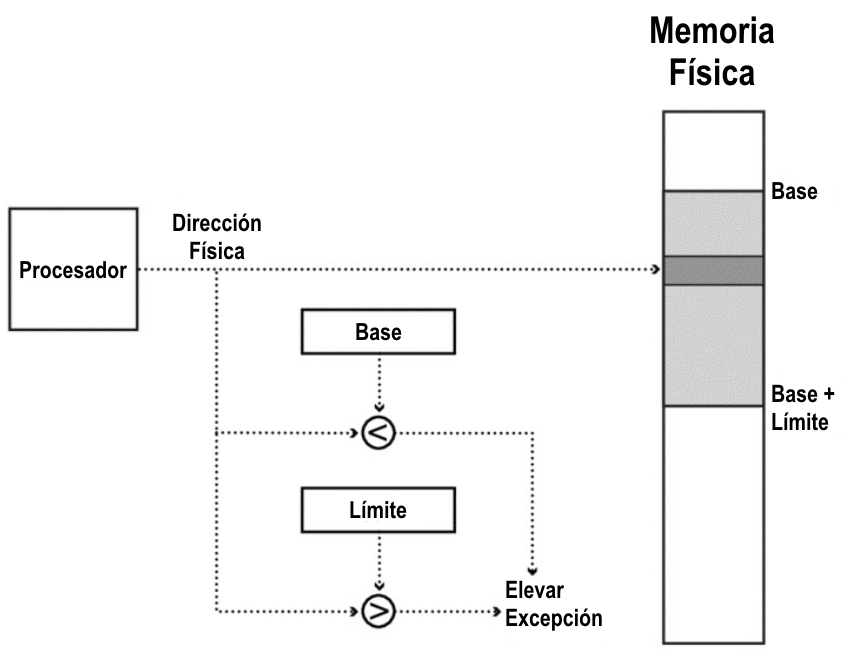
\includegraphics[scale=0.55]{img/fig0203}}
\caption{Método Base-Límite de protección de memoria usando direcciones físicas.}
\label{fig0203}
\end{figure}

Cada vez que el procesador obtiene una instrucción, se comprueba la dirección del contador de programa para ver si está entre los registros base y límite. Si es así, se permite proceder a la instrucción FETCH (obtener/traer); de otro modo, el hardware genera una excepción, se suspende el programa y se transfiere el control de vuelta al kernel del sistema operativo. Del mismo modo, para instrucciones que leen o escriben datos en la memoria, el procesador comprueba cada referencia a la memoria contra los registros base y límite, lo que genera una excepción de procesador si se violan los límites.

El kernel del sistema operativo se ejecuta sin los registros base y límite, lo que le permite acceder a cualquier memoria en el sistema - la memoria del kernel o la memoria de cualquier proceso de aplicación que se ejecuta en el sistema. Dado que las aplicaciones tocan sólo su propia memoria, el núcleo debe copiar explícitamente cualquier entrada o salida dentro o fuera de la región de memoria de la aplicación..

El uso de los registros base y límite, direccionados físicamente, puede proporcionar protección pero esto no proporciona algunas características importantes:

\begin{itemize}
\item \textbf{\textit{Heap} y pila expandibles}: con un sólo par de registros base y límite por cada proceso, la cantidad de memoria asignada a un programa se fija cuando se inicia el programa.
\item \textbf{Memoria compartida}: los registros base y límite no permiten que la memoria sea compartida entre los diferentes procesos, como sería útil, por ejemplo, para compartir código entre múltiples procesos que ejecutan el mismo programa o usan la misma biblioteca.
\item \textbf{Direcciones de memoria física}: cada programa se carga en la memoria física en tiempo de ejecución y debe utilizar esas direcciones de memoria física. Puesto que un programa puede ser cargado en diferentes lugares dependiendo de qué otros programas se estén ejecutando al mismo tiempo, el kernel debe cambiar la ubicación de cada instrucciones y dato que referencie a una dirección global, cada vez que el programa se carga en memoria.
\item \textbf{Fragmentación de memoria}: Una vez que se inicia un programa, es casi imposible reubicarlo. El programa podría almacenar punteros en los registros o en la pila de ejecución y estos punteros necesitan ser cambiados para mover el programa a una región diferente de la memoria física. Con el tiempo, a medida que las aplicaciones comienzan y terminan en tiempos irregulares, la memoria se fragmentará cada vez más. Potencialmente, la fragmentación de memoria puede llegar a un punto donde no hay suficiente espacio contiguo para iniciar un nuevo proceso, a pesar de suficiente memoria libre en su conjunto.
\end{itemize}

Por estas razones, la mayoría de los procesadores modernos introducen un nivel de indirección, denominado \textbf{direcciones virtuales}. Con direcciones virtuales, la memoria de cada proceso se inicia en el mismo lugar, por ejemplo, cero. Cada proceso cree que tiene toda la máquina para sí aunque, obviamente, esto no sea la realidad. El hardware traduce estas direcciones virtuales a posiciones de memoria física. Las direcciones virtuales también pueden dejar que la pila y \textit{heap} comiencen en extremos separados del espacio de direcciones virtuales para que puedan crecer según las necesidades del programa. La expansión es completamente transparente para el proceso de usuario
 
Con direcciones virtuales, si varias copias de un programa se ejecutan simultáneamente, cada copia del programa imprimirá exactamente el mismo resultado. Esto sería imposible si cada copia se dirigiera directamente las posiciones de memoria física. En otras palabras, cada instancia del programa parece encontrarse en su propia copia completa de la memoria.


\subsection{Interrupciones del Temporizador}
El aislamiento de procesos también requiere que el hardware proporcione un forma para que el kernel del sistema operativo recupere periódicamente el control del procesador. Cuando el sistema operativo inicia un programa a nivel usuario, el proceso es libre de ejecutar cualquier instrucción a nivel usuario (sin privilegios), llamar a cualquier función en la región de memoria del proceso, cargar o almacenar cualquier valor a su memoria, etc. Para el programa de usuario esto se muestra como si tuviera control completo del hardware dentro de los límites de su región de memoria.

Sin embargo, esto también es sólo una ilusión. Si la aplicación entra en un bucle infinito, o si el usuario simplemente se vuelve impaciente y quiere que el sistema detenga la aplicación, a continuación, el sistema operativo debe ser capaz de recuperar el control. Por supuesto, el sistema operativo necesita para ejecutar instrucciones decidir si se debe detener la aplicación, pero si la aplicación controla el procesador, el sistema operativo, por definición, no se está ejecutando en dicho procesador.

El sistema operativo también tiene que recuperar el control del procesador en funcionamiento normal. Supongamos que el usuario está ejecutando varias aplicaciones al mismo tiempo. Para que funcionen sin problemas estas aplicaciones y para responder de manera oportuna a la entrada del usuario, el sistema operativo debe ser capaz de recuperar el control para cambiar a una nueva tarea.

Casi todos los sistemas informáticos incluyen un dispositivo llamado \textbf{temporizador de hardware}, que se puede ajustar para interrumpir el procesador después de un retardo especificado (ya sea en el tiempo o después de que algún número de instrucciones haya sido ejecutadas). Cada temporizador interrumpe sólo un procesador, por lo que un multiprocesador por lo general tendrá un temporizador independiente para cada CPU. El sistema operativo puede configurar cada temporizador de expirar cada pocos milisegundos; tiempo de reacción humano es de unos pocos cientos de milisegundos. El restablecimiento del temporizador es una operación privilegiada, accesible sólo dentro del kernel, para que el proceso a nivel de usuario no puede inadvertidamente o maliciosamente desactivar el temporizador.

Cuando se produce la interrupción de temporizador, el hardware transfiere el control del proceso de usuario al kernel. Un temporizador u otra interrupción no implica que el programa tenga un error; en la mayoría de los casos, después de restablecer el temporizador, el sistema operativo reanuda la ejecución del proceso, estableciendo el modo, contador de programa y registros de nuevo a los valores que tenían inmediatamente antes se produjera la interrupción.

\section{Tipos de Modo de Transferencia}

Una vez que el núcleo ha colocado un proceso de usuario en un entorno limitado cuidadosamente construido, la siguiente pregunta es cómo hacer la transición con seguridad de la ejecución de un proceso de usuario para ejecutar el kernel, y viceversa. Estas transiciones no son eventos raros. Un servidor web de alto rendimiento, por ejemplo, puede cambiar entre el modo usuario y modo kernel miles de veces por segundo. Por lo tanto, el mecanismo debe ser a la vez rápido y seguro, sin dejar espacio para programas maliciosos o con errores de corromper el kernel, ya sea intencional o inadvertidamente.

\subsection{Del modo Usuario al modo Kernel}

Hay tres razones para que el kernel tome el control de un proceso de usuario: \textbf{interrupciones}, \textbf{excepciones del procesador}, y las \textbf{llamadas al sistema}. Las interrupciones se producen de forma asíncrona - es decir, que son provocados por un evento externo y pueden causar una transferencia al modo kernel después de cualquier instrucción de modo de usuario. Las excepciones del procesador y las llamadas al sistema son eventos síncronos activados por la ejecución del proceso. Utilizamos el término \textit{trap} para referirse a cualquier transferencia sincrónica de control desde el modo de usuario al kernel; Algunos sistemas utilizan el término más genérico para cualquier transferencia del control de un nivel menos privilegiada a un nivel más alto.

\begin{itemize}
\item \textbf{Interrupciones.} Una interrupción es una señal asíncrona al procesador que algún evento externo produce y que pueden requerir su atención. A medida que el procesador ejecuta las instrucciones, comprueba si ha llegado una interrupción. Si es así, se completan o se detienen todas las instrucciones que están en curso. En lugar de ir a buscar la siguiente instrucción, el hardware del procesador guarda el estado de ejecución actual y comienza a ejecutar en un controlador de interrupciones especialmente designado en el núcleo. En un multiprocesador, una interrupción se toma en sólo uno de los procesadores; los demás siguen ejecutando como si nada hubiera pasado.

Cada tipo diferente de interrupción requiere su propio controlador. Para interrupciones del temporizador, el controlador comprueba si el proceso actual está siendo sensible a la entrada del usuario para detectar si el proceso ha entrado en un bucle infinito. El controlador del temporizador también puede conmutar la ejecución de un proceso diferente para asegurarse de que cada proceso tiene un turno. Si no es necesario ningún cambio, el controlador de temporizador reanuda la ejecución en la instrucción interrumpida, de forma transparente para el proceso de usuario.

Las interrupciones también se utilizan para informar al núcleo de la finalización de solicitudes de E/S. Por ejemplo, el hardware del dispositivo del ratón provoca una interrupción cada vez que el usuario se mueve o hace click. El núcleo, a su vez, notifica al proceso de usuario adecuado - al que el usuario estaba "pasando el ratón por encima". Prácticamente, para todos los dispositivos de E/S (Ethernet, WiFi, disco duro, unidad de disco USB, teclado, ratón) se genera una interrupción cada vez que llega alguna entrada para el procesador y cada vez que una solicitud esta completa.

Una alternativa a las interrupciones es la votación: los bucles del núcleo, comprobando cada dispositivo de E/S para ver si se ha producido un evento que requiere la manipulación. No se necesita saber, si el núcleo es de votación, no está disponible para ejecutar código a nivel de usuario.

Las interrupciones entre procesadores, son otra fuente de interrupciones. Un procesador puede enviar una interrupción para cualquier otro procesador. El núcleo utiliza estas interrupciones para coordinar acciones en todo el multiprocesador; por ejemplo, cuando un programa paralelo sale, el núcleo envía interrupciones para detener el programa y de continuar para funcionar en cualquier otro procesador.

\item \textbf{Excepciones del Procesador.} Una excepción del procesador es un evento de hardware causado por el comportamiento del programa de usuario que provoca una transferencia de control al kernel. Al igual que con una interrupción, el hardware termina todas las instrucciones anteriores, guarda el estado de ejecución actual, y comienza a correr a un gestor de excepciones especialmente designado en el núcleo. Por ejemplo, una excepcion de procesador se produce cuando un proceso intenta realizar una instrucción privilegiada o accede a la memoria fuera de su propia región de memoria. Otras excepciones del procesador se producen cuando un proceso divide un número entero  por cero, accede a una palabra de memoria con una dirección no alineada, intenta escribir en memoria de sólo lectura, y así sucesivamente. En estos casos, el sistema operativo simplemente detiene el proceso y devuelve un código de error al usuario. En un multiprocesador, la excepción sólo detiene la ejecución en el procesador en el cual se desencadena la excepción; Así, el núcleo necesita enviar interrupciones entre procesadores para detener la ejecución del programa paralelo en otros procesadores.

Las excepciones del procesador también son causados por los eventos mas benignos del programa. Por ejemplo, para establecer un punto de interrupción en un programa, el núcleo sustituye a la instrucción de máquina en la memoria con una instrucción especial que invoca una \textit{trap}. Cuando el programa llega a ese momento de su ejecución, el hardware cambia al modo kernel. El núcleo restaura la instrucción de edad y transfiere el control al depurador. El depurador puede examinar las variables del programa, establecer un nuevo punto de interrupción y reanudar el programa en la operación causando la excepción.

\item \textbf{Las Llamadas al Listema.} Los procesos de usuario también pueden hacer la transición hacia el núcleo del sistema operativo de forma voluntaria al solicitar que los kernel realicen una operación en nombre del usuario. Una llamada al sistema es cualquier procedimiento previsto por el núcleo que se puede llamar desde el nivel del usuario. La mayoría de los procesadores implementan las llamadas al sistema con una trampa \textit{trap} o instrucción de llamada al sistema. Sin embargo, no es estrictamente necesario una instrucción especial; en algunos sistemas, un proceso desencadena una llamada al sistema mediante la ejecución de una instrucción con un código de operación no válido específico.

Al igual que con una interrupción o una excepción de procesador, la instrucción \textit{trap} cambia el modo del procesador del usuario al núcleo y se inicia la ejecución en el núcleo de un controlador predefinido. Para proteger el núcleo de los programas de usuario maliciosos, es esencial que las transferencias de control de hardware en un sistema de llamadas en una dirección predefinida - los procesos de usuario no pueden saltar a puntos arbitrarios del núcleo.

Los sistemas operativos pueden proporcionar cualquier número de llamadas al sistema. Los ejemplos incluyen llamadas al sistema para establecer una conexión con un servidor web, para enviar o recibir paquetes a través de la red, para crear o borrar archivos, para leer o escribir datos en archivos, y crear un nuevo proceso de usuario. Para el programa de usuario, estos se denominan como los procedimientos normales, con parámetros y valores de retorno. La persona que llama tiene que estar preocupada sólo con la interfaz; no necesita saber que la rutina en realidad está siendo implementada por el núcleo. El kernel se encarga de los detalles del control y de la copia de argumentos, la realización de la operación, y los valores de retorno de copia de nuevo en la memoria del proceso. Cuando el núcleo completa la llamada al sistema, se reanuda la ejecución a nivel de usuario en la instrucción inmediatamente después de la \textit{trap}.
\end{itemize}

\subsection{Del modo Kernel al modo Usuario}
Hay varias razones por las cuales se puede pasar del modo kernel al modo usuario:

\begin{itemize}
\item \textbf{Nuevo proceso.} Para iniciar un nuevo proceso, el núcleo copia el programa en la memoria, define el contador de programa a la primera instrucción del proceso, define el puntero de pila a la base de la pila de usuario, y cambia al modo de usuario.

\item \textbf{Reanudar después de una interrupción, excepción del procesador, o llamada al sistema.} Cuando el núcleo termina controla la solicitud, se reanuda la ejecución del proceso interrumpido por la restauración de su contador de programa (en el caso de una llamada al sistema, la instrucción después de la \textit{trap}), la restauración de sus registros, y cambiar el modo de nuevo a nivel de usuario.

\item \textbf{Cambiar a un proceso diferente.} En algunos casos, como en una interrupción del temporizador, el núcleo cambia a un proceso diferente que el que había estado funcionando antes de la interrupción. Puesto que el núcleo finalmente reanuda el proceso anterior, el núcleo necesita salvar el estado del proceso - el contador de programa, registros, y así sucesivamente - en el bloque de control del proceso. El núcleo puede reanudar un proceso de carga diferente de su estado - su contador de programa, registros, y así sucesivamente - a partir del bloque de control de proceso en el procesador y luego cambiar a modo de usuario.

\item \textbf{Llamada scendente a nivel de usuario.} Muchos sistemas operativos proporcionan programas de usuario con la capacidad de recibir notificación asíncrona de los acontecimientos.
\end{itemize}

\section{Implementación de la Transferencia en Modo Seguro}
Tanto para la transición de usuario al modo kernel o en la dirección opuesta, se debe tener cuidado para asegurar que un programa de usuario malicioso no pueda corromper el núcleo. Aunque la idea básica es simple, la implementación de bajo nivel puede ser un poco compleja: el procesador debe guardar su estado y cambiar lo que está haciendo, durante la ejecución de las instrucciones que pueda alterar el estado que se encuentra en el proceso de ahorro.

El código de cambio de contexto debe ser cuidadosamente diseñado, y se apoya en el soporte de hardware. Para evitar la confusión y reducir la posibilidad de error, la mayoría de sistemas operativos tienen una secuencia común de instrucciones tanto para entrar en el núcleo - ya sea debido a las interrupciones, excepciones del procesador o sistema llama - y para regresar a nivel de usuario, de nuevo, independientemente de la causa.

Como mínimo, esta secuencia común debe proporcionar:
\begin{itemize}
\item \textbf{La entrada limitada en el núcleo.} Para transferir el control al núcleo del sistema operativo, el hardware debe asegurar que el punto de entrada en el núcleo es puesto en marcha por el núcleo. Los programas de usuario no pueden saltar a cualquier ubicación en el núcleo. Por ejemplo, el código del núcleo para manejar el sistema de archivos de lectura primero comprueba si el programa de usuario tiene permiso para hacerlo. Si no, el núcleo debe devolver un error. Sin puntos de entrada limitados en el núcleo, un programa malicioso podría saltar inmediatamente después del código para realizar la verificación, permitiendo que el programa pueda acceder a algún otro archivo.

\item \textbf{Cambios atómicos en el estado del procesador.} En el modo de usuario, el contador de programa y el punto de pila de posiciones de memoria en el proceso de usuario; la protección de la memoria impide al proceso usuario acceder a cualquier memoria fuera de su región. En el modo de núcleo, el contador de programa y el punto de pila de posiciones de memoria en el núcleo; la protección de la memoria se cambia para permitir que el kernel pueda acceder tanto a sus propios datos y la del proceso de usuario. La transición entre los dos es atómica - el modo, contador de programa, pila, y la protección de la memoria se cambiaron todos al mismo tiempo.

\item \textbf{Transparente, la ejecución puede reiniciar.} Un evento puede interrumpir un proceso a nivel de usuario en cualquier momento, entre cualquier instrucción y la siguiente. Por ejemplo, el procesador podría haber calculado una dirección de memoria, cargado en un registro, y estar a punto de almacenar un valor en esa dirección. El sistema operativo debe ser capaz de restaurar el estado del programa de usuario exactamente como era antes de que ocurriera la interrupción. Para el proceso de usuario, una interrupción es invisible, a excepción de que el programa se desacelera temporalmente.

En una interrupción, el procesador guarda su estado actual en la memoria, de manera temporal difiere más eventos, cambios al modo kernel, y luego salta al manipulador de interrupciones o excepciones. Cuando el manipulador termina, los pasos se invierten: el estado del procesador se restaura desde su ubicación guardada, con el programa interrumpido sin enterarse.
\end{itemize}

Con ese contexto, ahora se describe el mecanismo de hardware y software para el manejo de una interrupción, a excepción del procesador, o llamada al sistema. Más tarde, reutilizamos este mismo mecanismo básico como un bloque de construcción para la implementación de las señales de nivel de usuario.

\subsection{Tabla vectorial de interrupción}
Cuando se produce una interrupción \textit{trap}, a excepción del procesador o llamada al sistema, el sistema operativo debe tomar acciones diferentes dependiendo de si el evento es una excepción de división por cero, una llamada al sistema para leer el archivo, o una interrupción del temporizador. ¿Cómo sabe el procesador qué código se ejecuta?
\begin{figure}[tbhp]
\centerline{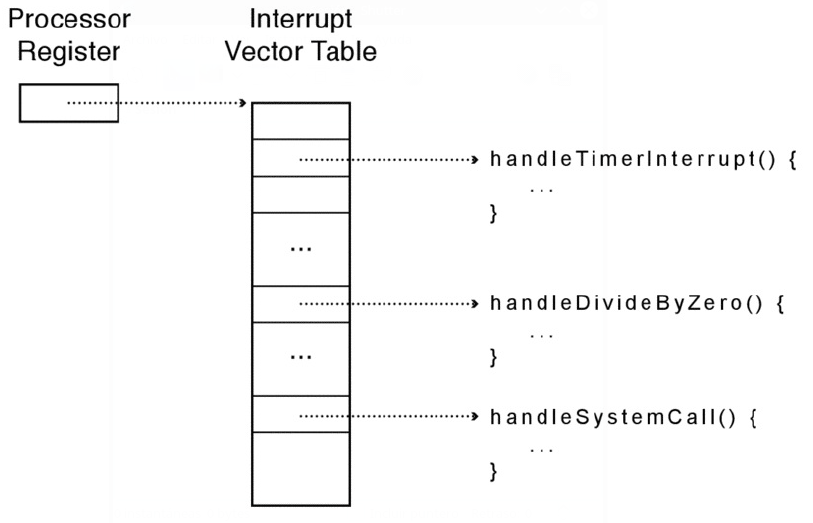
\includegraphics[scale=0.55]{img/fig05}}
\caption{Tabla vectorial de interrupciones: se enumeran las rutinas del núcleo para manejar varias interrupciones de hardware, excepciones del procesador, y las llamadas al sistema.}
\label{fig0}
\end{figure}

Como ilustra la figura, el procesador tiene un registro especial que apunta a un área de memoria del núcleo llamada la tabla vectorial de interrupciones. La tabla vectorial de interrupciones es una matriz de punteros, con cada entrada que apunta a la primera instrucción de un procedimiento controlador diferente en el núcleo. Un manejador de interrupciones es el término usado para el procedimiento llamado por el núcleo de una interrupción.

El formato de la tabla vectorial de interrupciones es específico del procesador. En el x86, por ejemplo, interrumpir entradas de la tabla vectorial $0-31$ son para diferentes tipos de excepciones del procesador (por ejemplo, división por cero); entradas de $32 - 255$ son de diferentes tipos de interrupciones (temporizador, teclado, etc.); y, por convención, la entrada $64$ apunta al controlador de la llamada al sistema \textit{trap}. El hardware determina qué dispositivo de hardware ha causado la interrupción, si la instrucción \textit{trap} fue ejecutada, o qué condición de excepción ocurrió. De este modo, el hardware puede seleccionar la entrada de la derecha de la tabla de interrupciones e invocar el manejador apropiado.

Algunos otros procesadores tienen un menor número de puntos de entrada, en lugar de poner un código que indica la causa de la interrupción en un registro especial de hardware. En ese caso, el software del sistema operativo utiliza el código para indexar en la tabla de interrupciones.

\subsection{Pila de Interrupciones}
Donde se debe guardar el estado del proceso interrumpido, y el código del kernel que la pila debe usar?

En la mayoría de los procesadores, puntos privilegiados de registro de hardware a una región de la memoria del núcleo llamado pila de interrupción. Cuando una interrupción \textit{trap}, a excepción del procesador, o llamada al sistema provoca un cambio de contexto en el núcleo, el hardware cambia el puntero de pila para que apunte a la base de la pila de interrupción del núcleo. El hardware guarda automáticamente algunos de los registros del proceso interrumpido empujándolos en la pila de interrupción antes de llamar al controlador del núcleo.

Cuando se ejecuta el controlador de kernel, empuja cualquier registros restantes en la pila antes de realizar su trabajo. Al regresar de la interrupción \textit{trap}, a excepción del procesador o llamada al sistema, ocurre lo contrario: en primer lugar, el controlador hace estallar los registros guardados y, a continuación, el hardware restaura los registros salvados, volviendo al punto en que se interrumpió el proceso. Al regresar de una llamada al sistema, el valor del contador de programa guardado se debe incrementar de modo que el hardware vuelve a la instrucción inmediatamente después de la que causó la \textit{trap}.

Se podría pensar que usted podría utilizar la pila a nivel proceso de usuario para almacenar su estado. Sin embargo, se necesita una, pila de interrupción a nilve kernel separado por dos razones.

\begin{itemize}
\item \textbf{Confiabilidad.} Un puntero de pila a nivel proceso de usuario podría no ser una dirección de memoria válida (por ejemplo, si el programa tiene un error), pero el controlador del núcleo debe seguir trabajando correctamente.

\item \textbf{Seguridad.} En un multiprocesador, otros subprocesos que se ejecutan en el mismo proceso pueden modificar la memoria del usuario durante la llamada al sistema. Si el controlador del núcleo almacena sus variables locales en la pila a nivel de usuario, el programa de usuario puede ser capaz de modificar la dirección del remitente del núcleo, que puede causar el kernel para saltar al código arbitrario.
\end{itemize}

En un multiprocesador, cada procesador tiene que tener su propia pila de interrupción de modo que, por ejemplo, el núcleo puede manejar llamadas simultáneas y excepciones del sistema a través de múltiples procesadores. Para cada procesador, el núcleo asigna una región separada de la memoria como pila de interrupción de dicho procesador.

\subsection{Dos Pilas por Proceso}
La mayoría de los núcleos de sistema operativo van un paso más allá y asignan una pila del núcleo de interrupción para cada proceso a nivel de usuario (y como veremos en el capítulo 4, cada subproceso que ejecuta código de usuario). Cuando un proceso a nivel de usuario se está ejecutando, la pila de interrupción de hardware apunta a la pila del núcleo de ese proceso. Tenga en cuenta que cuando un proceso está funcionando a nivel de usuario, no se está ejecutando en el núcleo por lo que su pila del núcleo está vacía.

La asignación de la pila del nucleo por proceso hace que sea más fácil cambiar a un nuevo proceso dentro de un manejador de interrupciones o una llamada al sistema. Por ejemplo, un controlador de interrupción de temporizador podría decidir dar el procesador a un proceso diferente. Del mismo modo, una llamada al sistema tenga que esperar a que una operación de E/S para completar; Mientras tanto, algún otro proceso debe ejecutarse. Con pilas por proceso, de suspender un proceso, almacenamos un puntero a su pila del núcleo en el bloque de control de proceso, y cambiar a la pila del nuevo proceso.

\begin{figure}[tbhp]
\centerline{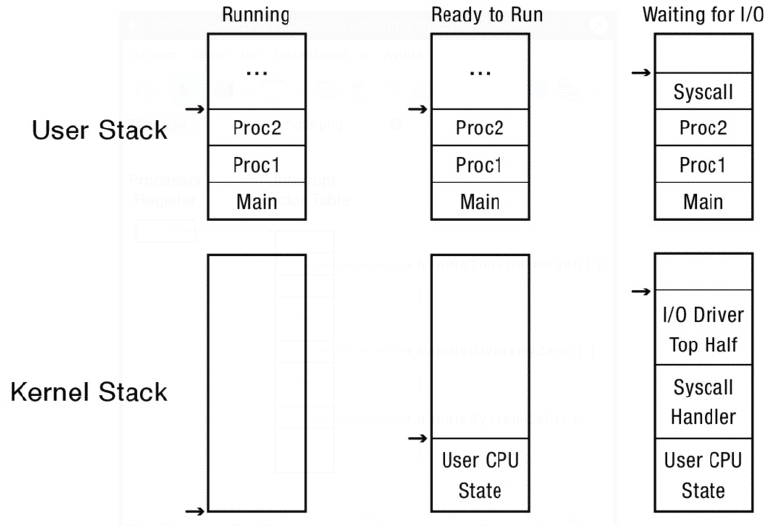
\includegraphics[scale=0.55]{img/fig06}}
\caption{En la mayoría de sistemas operativos, un proceso tiene dos pilas: una para ejecutar código de usuario y una para el código del kernel.}
\label{fig06}
\end{figure}

La figura muestra las pilas del núcleo y de usuario para varios estados de un proceso. Cuando un proceso se ejecuta en modo usuario, su pila del núcleo está vacía. Cuando un proceso ha sido apropiado (listo pero no en funcionamiento), la pila del núcleo contendrá el estado del procesador a nivel de usuario en el momento en que el proceso de usuario se interrumpió. Cuando un proceso se encuentra dentro de una llamada al sistema espera de E/S, la pila del núcleo contiene el contexto de reanudarse cuando la E/S completa, y la pila de usuario contiene el contexto de reanudarse cuando vuelva la llamada al sistema. 

La figura resume los diversos estados de pilas de usuario y núcleo de un proceso:
\begin{itemize}
\item Si el proceso se está ejecutando en el procesador en modo de usuario, su pila del núcleo está vacía, lista para ser usada por una interrupción, a excepción del procesador, o llamada al sistema.

\item Si el proceso se está ejecutando en el procesador en modo de núcleo - debido a una llamada de interrupción, a excepción del procesador o del sistema - El kernel está en uso, que contiene los registros guardados de la computación a nivel de usuario en suspensión, así como el estado actual del kernel entrenador de animales.

\item Si el proceso está disponible para funcionar, pero está esperando su turno en el procesador, la pila del núcleo contiene los registros y estado para ser restaurados cuando se reanude el proceso.

\item Si el proceso está esperando un evento de E/S para completar, su pila del núcleo contiene el cómputo suspendido para ser reanudado cuando la E/S finaliza.
\end{itemize}

\subsection{El enmascaramiento de interrupciones}
Las interrupciones llegan de forma asíncrona; el procesador podría estar ejecutando un código usuario o un código del núcleo cuando llega una interrupción. En ciertas regiones del kernel -como manejador de interrupciones dentro de ellos mismos, o dentro del planificador de la CPU- teniendo una interrupción podría causar confusión. Si se interrumpe un manejador de interrupciones, no podemos establecer el puntero de pila para que apunte a la base de la pila de interrupción del núcleo -de este modo destruiría el estado de la primera rutina de tratamiento.

Para simplificar el diseño del núcleo, el hardware proporciona una instrucción privilegiada, \textit{aplazar} temporalmente la entrega de una interrupción hasta que sea seguro hacerlo. Para el x$86$ y varios otros procesadores, esta instrucción se llama interrupciones con movilidad reducida. Sin embargo, este es un término equivocado: la interrupción solo se aplaza (enmascarado), y no hizo caso. Una vez que se ejecuta una instrucción correspondiente habilitar las interrupciones, las interrupciones pendientes se entregan al procesador. Las instrucciones para enmascarar y desenmascarar interrupciones deben ser privilegiadas; de lo contrario, podría un código de usuario inadvertidamente o maliciosamente desactivar el temporizador de hardware, permitiendo que la máquina se congele.

Si llegan múltiples interrupciones, mientras que las interrupciones están deshabilitadas, el hardware las enviará cuando se vuelven a habilitar las interrupciones. Sin embargo, puesto que el hardware tiene búfer limitado por las interrupciones pendientes, algunas interrupciones se pueden perder si están deshabilitadas por un período demasiado largo de tiempo. En general, el hardware retendrá una interrupción de cada tipo; el manejador de interrupciones es responsable de comprobar el hardware del dispositivo para ver si hay varios eventos de E / S pendientes necesitan ser procesados.

Si el procesador realiza una interrupción en modo kernel con las interrupciones habilitadas, es seguro de usar el puntero de pila actual en lugar de que se quede en la base de la pila de interrupción. Este enfoque puede empujar de forma recursiva una serie de estados manipuladores en la pila; a continuación, ya que cada uno completa, su estado se extrae de la pila, y el manejador anterior se reanuda donde se quedó.

\subsection{Soporte de Hardware para el Ahorro y Restauración de Registros}
Los registros de un proceso interrumpido deben guardarse para que el proceso se pueda reiniciar exactamente donde se lo dejó. Debido a que el controlador puede cambiar los valores de los registros conforme se ejecuta, el estado debe guardarse antes de que acabe el manejador. Debido a que la mayoría de las instrucciones modifican los contenidos de los registros, el hardware suele proporcionar instrucciones especiales para que sea más fácil de guardar y restaurar el estado de usuario.

Para hacer esto concreto, tenga en cuenta la arquitectura x$86$. En lugar de confiar en el software de controlador para hacer todo el trabajo, cuando se produce una interrupción o una \textit{trap}:
\begin{itemize}
\item Si el procesador está en modo de usuario, el $86$ empuja el puntero de pila del proceso interrumpido en la pila de interrupción del núcleo y pasa a la pila del núcleo.

\item El $86$ empuja puntero de instrucción del proceso interrumpido.

\item El $86$ empuja la palabra de estado del procesador x$86$. La palabra de estado del procesador incluye bits de control, tales como si la última operación aritmética en el código interrumpido resultó en un valor negativo, positivo o cero. Esto necesita ser salvado y restaurado para el comportamiento correcto de cualquier instrucción de salto condicional posterior.
\end{itemize}

El hardware guarda los valores para el puntero de pila, contador de programa, y la palabra de estado del procesador antes de saltar a través de la tabla de vectores de interrupción al controlador de interrupciones. Una vez que el controlador se pone en marcha, estos valores serán las del controlador, no los del proceso interrumpido.

Una vez que el controlador se pone en marcha, se puede utilizar el \textit{pushad} (empujar todas dobles) la orden de guardar los registros restantes en la pila. Esta instrucción se guarda todos los registros x$86$ enteros de $32$ bits. En un x$86$ de $16$ bits, \textit{pusha} se utiliza en su lugar. Dado que el núcleo no suele realizar operaciones de punto flotante, los que no tienen que ser salvados a menos que el kernel cambie a un proceso diferente.

La arquitectura x$86$ tiene características complementarias para la restauración de estado: una instrucción \textit{POPAD} para hacer estallar una serie de valores de los registros enteros de la pila en los registros y un iret (return from interrupt - regreso de interrupción) de instrucciones que carga un puntero de pila, puntero de instrucción, y la palabra de estado del procesador fuera de la pila en los registros del procesador apropiados.

\section{Poniendo todo junto: Modo de Transferencia x86}
Los pasos de alto nivel necesarios para manejar una interrupción, a excepción del procesador, o llamada al sistema son simples, pero los detalles requieren algún tipo de atención.

Para dar un ejemplo concreto de cómo tales "cuidadosamente elaboradas" código funciona, ahora describen una forma de implementar un cambio de modo de interrupción activada por en la arquitectura x86. Los diferentes sistemas operativos en el x86 siguen este enfoque básico, aunque los detalles difieren. Del mismo modo, diferentes arquitecturas manejan los mismos tipos de problemas, pero pueden hacerlo con el soporte de hardware diferente.

En primer lugar, proporcionamos algunos antecedentes en la arquitectura x$86$. El $86$ está segmentado, por lo que los punteros vienen en dos partes: $(i)$ un segmento, una región de memoria tal como código, datos, o la pila, y $(ii)$ un desplazamiento dentro de ese segmento. La instrucción en curso a nivel de usuario es una combinación del segmento de código (registro \textit{CS}) más el puntero de instrucción (registro \textit{EIP}). Del mismo modo, la posición actual de la pila es la combinación de segmento de pila (\textit{ss}) y el puntero de pila dentro del segmento de pila (\textit{esp}). El nivel de privilegio actual es almacenado como los bits de orden inferior del registro \textit{CS} en lugar de en la palabra de estado del procesador (registro \textit{eflags}). El registro tiene eflags códigos de condición que se modifican como un subproducto de la ejecución de las instrucciones; los eflags registrar también tiene otros indicadores que controlan el comportamiento del procesador, como por ejemplo cuando las interrupciones están enmascarados o no.

\begin{figure}[tbhp]
\centerline{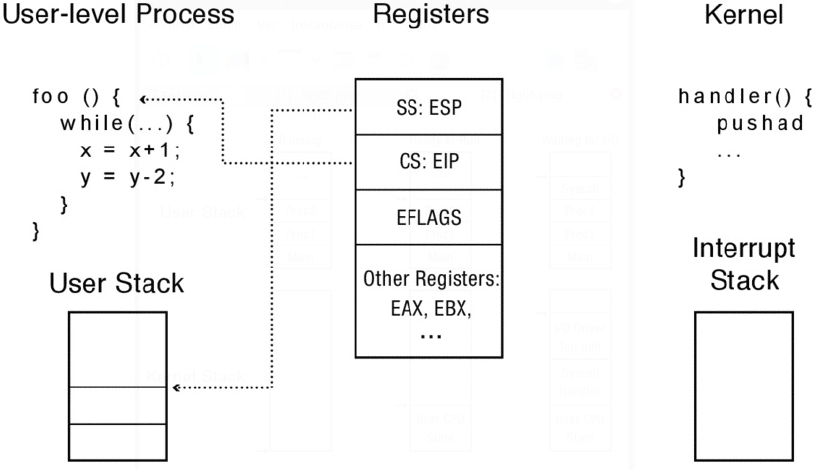
\includegraphics[scale=0.55]{img/fig07}}
\caption{Estado del sistema antes de un manejador de interrupciones se invoca en la arquitectura x86. SS es el segmento de pila, ESP es el puntero de pila, CS es el segmento de código, y EIP es el contador de programa. El contador de programa y puntero de pila se refiere a lugares en el proceso de usuario, y la pila de interrupción está vacía.}
\label{fig07}
\end{figure}

Cuando un proceso a nivel de usuario está en ejecución, el estado actual del procesador, pila, la tabla vectorial de interrupciones del núcleo, y la pila del núcleo se ilustra en la \textit{fig.} \ref{fig07}. Cuando se produce una \textit{trap} a excepción del procesador o llamada al sistema, el hardware ahorra cuidadosamente una pequeña cantidad del estado de rosca interrumpida, que sale del sistema como se muestra en la \textit{fig.} \ref{fig08}:

\begin{figure}[tbhp]
\centerline{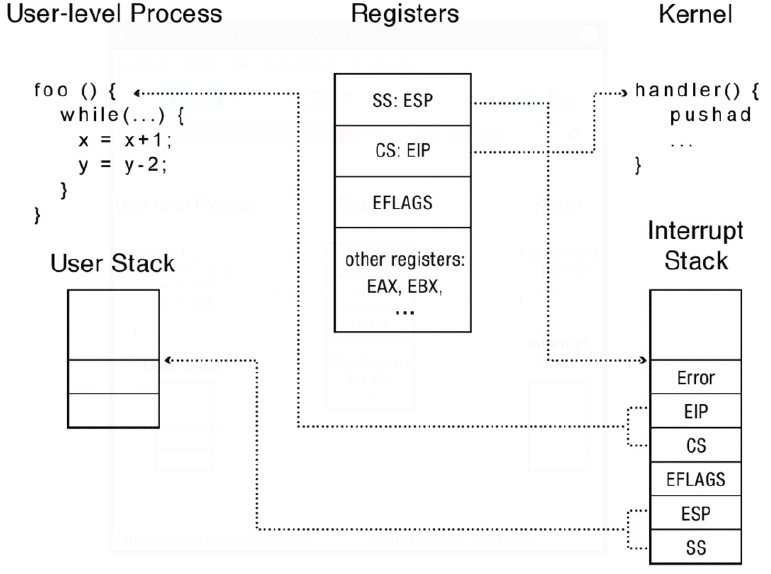
\includegraphics[scale=0.55]{img/fig08}}
\caption{Estado del sistema después de que el hardware x$86$ ha saltado al manejador de interrupciones. El hardware ahorra el contexto de usuario en la pila de interrupción del núcleo y cambia el contador de programa / pila a ubicaciones en la memoria del núcleo.}
\label{fig08}
\end{figure}

\begin{enumerate}
\item \textbf{Enmascaramiento de interrupciones.} El hardware se inicia mediante la prevención de las interrupciones que se produzcan mientras el procesador está en el medio de cambiar de modo de usuario al modo kernel.

\item \textbf{Guardar tres valores clave.} El hardware guarda los valores del puntero de pila (ESP x86 y registros ss), las banderas de ejecución (los eflags x86 registro), y el puntero de instrucción (EIP x86 y registros cs) a los registros de hardware internos, temporales.

\item \textbf{Cambiar a la pila de interrupción del núcleo.} El hardware entonces cambia el puntero del segmento de pila / pila a la base de la pila de interrupción del núcleo, tal como se especifica en un registro especial de hardware.

\item \textbf{Empuje los tres valores clave en la nueva pila.} A continuación, el hardware almacena internamente los valores guardados en la pila.

\item \textbf{Opcionalmente guardar un código de error.} Ciertos tipos de excepciones, tales como fallos de página, generan un código de error para proporcionar más información sobre el evento; para estas excepciones, el hardware empuja este código, por lo que es el primer elemento en la pila. Para otros tipos de eventos, el software de controlador de interrupción empuja un valor ficticio en la pila de forma que el formato de pila es idéntico en ambos casos.

\item \textbf{Invocar el manejador de interrupciones.} Por último, el hardware cambia el contador de código egment / programa a la dirección del procedimiento controlador de interrupciones. Un registro especial en el procesador contiene la ubicación de la tabla de vectores de interrupción en la memoria del núcleo. Este registro sólo puede ser modificada por el kernel. El tipo de interrupción se asigna a un índice de esta matriz, y el contador de segmento de código / programa se establece en el valor en este índice.
\end{enumerate}

Esto inicia el software de controlador.
El guía debe guardar primero el resto del estado del proceso interrumpido - que necesita para salvar a los otros registros antes de que los cambia! El controlador empuja el resto de los registros, incluyendo el puntero de pila actual, en la pila mediante la instrucción x$86$ \textit{PUSHAD}.

\begin{figure}[tbhp]
\centerline{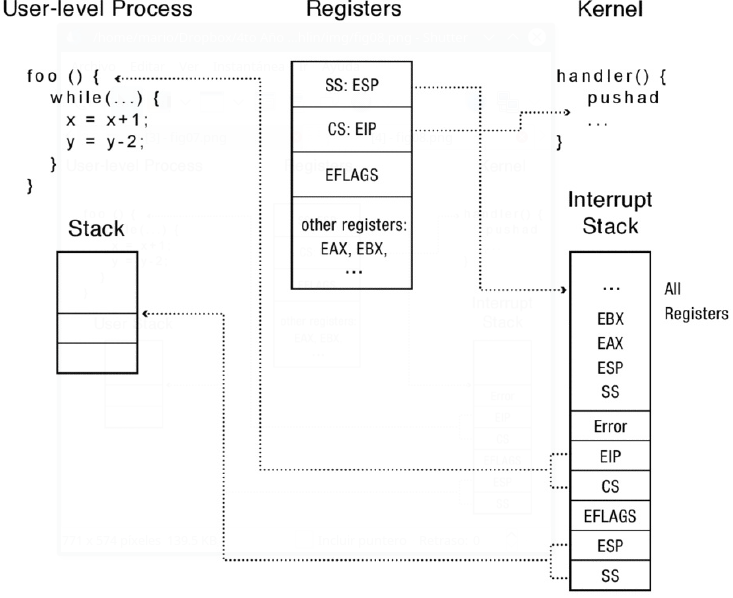
\includegraphics[scale=0.55]{img/fig09}}
\caption{ Estado del sistema después de que el controlador de interrupciones ha comenzado a ejecutar en la arquitectura x86. El controlador de guarda primero el estado actual de los registros del procesador, ya que puede sobrescribir ellos. Tenga en cuenta que esto ahorra el puntero de pila doble: en primer lugar, la pila de usuario puntero a continuación, el puntero de pila del núcleo.}
\label{fig09}
\end{figure}

Como muestra la \textit{fig.} \ref{fig09}, en este punto la pila de interrupción del núcleo posee $(1)$ el puntero de pila, banderas de ejecución, y el contador de programa guardada por el hardware, $(2)$ un código de error o valor ficticio, y $(3)$ una copia de todos los registros generales (incluyendo el puntero de pila, pero no el puntero de instrucción o eflags registro).

Una vez que el controlador ha estado guardado de la rosca interrumpida a la pila, puede utilizar los registros de lo que le plazca, y se puede desplazar objetos adicionales en la pila. Por lo tanto, el controlador puede ahora hacer cualquier trabajo que tiene que hacer.

Cuando el controlador se completa, se puede reanudar el proceso interrumpido. Para ello, el controlador hace estallar los registros se guardan en la pila. Esto restaura todos los registros, excepto las banderas de ejecución, contador de programa, y puntero de pila. Para el conjunto de instrucciones x$86$, la instrucción POPAD se utiliza comúnmente. El controlador también aparece el valor de error de la pila.

Por último, el controlador ejecuta la instrucción x$86$ \textit{iret} para restaurar el segmento de código, contador de programa, banderas de ejecución, segmento de pila, y el puntero de pila de pila de interrupción del núcleo.

Esto restaura el estado del proceso exactamente a lo que era antes de la interrupción. El proceso continúa la ejecución como si nada hubiera pasado.

Un pequeño pero importante detalle se produce cuando el hardware toma una excepción para emular una instrucción en el kernel, por ejemplo, por falta de hardware de punto flotante. Si el controlador vuelve de nuevo a la instrucción que provocó la excepción, otra excepción se repetiría al instante. Para evitar un bucle infinito, el gestor de excepciones modifica el contador de programa almacenado en la base de la pila para que apunte a la instrucción inmediatamente después el que causa el interruptor de modo. La instrucción \textit{iret} luego puede volver al proceso de usuario en la ubicación correcta.

Para una trampa llamada al sistema, el hardware x86 de Intel hace el incremento cuando se guarda el estado a nivel de usuario. El contador de programa para la instrucción después de la trampa se guarda en la pila de interrupción del núcleo.

\section{Implementación de las Llamadas al Sistema}
El núcleo del sistema operativo construye un entorno restringido para la ejecución de los procesos con el fin de limitar el impacto de los programas maliciosos y erróneos sobre la fiabilidad del sistema. Cada vez que un proceso necesita llevar a cabo una acción fuera de su dominio de protección -para crear un nuevo proceso, leer desde el teclado, o escribir un bloque en disco- debe pedir al sistema operativo que realice la acción en su nombre, a través de una llamada al sistema.

Las llamadas al sistema proporcionan la ilusión de que el núcleo del sistema operativo es simplemente un conjunto de rutinas de biblioteca disponibles para los programas de usuario. Para el programa de usuario, el kernel proporciona un conjunto de procedimientos de llamada del sistema, cada uno con sus propios argumentos y valores de retorno, que puede ser llamado como cualquier otra rutina. El programa de usuario no necesita preocuparse por cómo el núcleo implementa estas llamadas. 

La implementación de las llamadas al sistema requiere que el sistema operativo definia una convención de llamada, es decir, cómo nombrar las llamadas al sistema, pasar argumentos, y recibir valores de retorno a través del límite de usuario/kernel. Por lo general, el sistema operativo utiliza la misma convención que el compilador utiliza para los procedimientos normales, una combinación de paso de argumentos en los registros y en la pila de ejecución.

Una vez que los argumentos están en el formato correcto, el programa a nivel de usuario puede emitir una llamada al sistema mediante la ejecución de la instrucción \textit{trap} para transferir el control al núcleo. Las llamadas al sistema, al igual que las interrupciones y excepciones del procesador, comparten el mismo mecanismo para cambiar entre modo kernel y usuario. De hecho, la instrucción \textit{trao} x$86$ en el núcleo de una llamada al sistema se le llama \textit{int}, por interrupción de software.

En el interior del núcleo, un procedimiento implementa cada llamada al sistema. Este procedimiento se comporta exactamente como si la llamada fue hecha desde el interior del núcleo, pero con una notable diferencia: el núcleo debe poner en práctica sus llamadas al sistema de una manera que se protege de todos los errores y los ataques que podrían ser lanzados por el mal uso de la interfaz. Por supuesto, la mayoría de las aplicaciones utilizarán la interfaz correctamente. Sin embargo, los errores en un programa de aplicación no deben chocar el núcleo, y un virus de ordenador no deberá ser capaz de utilizar la interfaz de llamada al sistema para tomar el control del kernel. Uno puede pensar en esto como una versión extrema de programación defensiva: el núcleo siempre debe asumir que los parámetros pasados a una llamada del sistema están diseñados intencionalmente para ser tan dañino como sea posible.

Vamos a unir estos dos puntos de vista, el programa de usuario haciendo la llamada al sistema, y el núcleo implementando la misma, con un par de \textit{stubs} (talones). Un par de \textit{stubs} es un par de procedimientos que median entre dos ambientes, en este caso entre el programa de usuario y el núcleo. Los \textit{stubs} también median las llamadas de procedimiento entre los equipos en un sistema distribuido.

\begin{figure}[tbhp]
\centerline{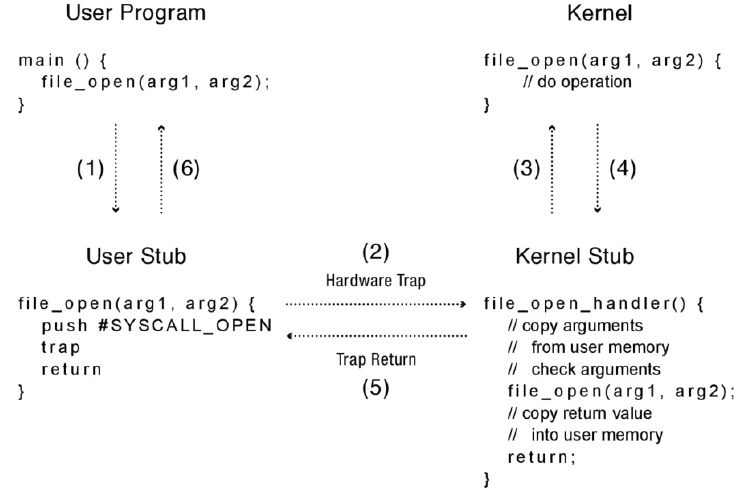
\includegraphics[scale=0.45]{img/fig10}}
\caption{Un par de \textit{stubs} media entre la llamada a nivel de usuario y la aplicación de la llamada en el núcleo. El código para la llamada al sistema es \textit{file \_ open}; otras llamadas tienen sus propios \textit{stubs}. $(1)$ El proceso de usuario realiza una llamada a procedimiento normal a un \textit{stub} vinculados con el proceso. $(2)$ El stub ejecuta la instrucción \textit{trap}. Esto transfiere el control al manejador \textit{trap} del kernel. Las copia al controlador \textit{trap} y comprueba sus argumentos y después $(3)$ llama a una rutina para hacer la operación. Una vez completada la operación, $(4)$ el código devuelve al controlador de la \textit{trap}, que copia el valor de retorno en la memoria de usuario y $(5)$ se reanuda el \textit{stub} del usuario inmediatamente después de la \textit{trap}. $(6)$ El \textit{stub} de usuario vuelve a la persona que llama a nivel de usuario.}
\label{fig10}
\end{figure}

La \textit{fig.} \ref{fig10} ilustra la secuencia de pasos que intervienen en una llamada al sistema:
\begin{enumerate}
\item El programa de usuario llama al talón de usuario en la forma normal, ajeno al hecho de la puesta en práctica del procedimiento es, de hecho, en el núcleo.
\item El talón de usuario rellena el código de la llamada al sistema y ejecuta la instrucción trampa.
\item Las transferencias de hardware de control en el núcleo, vectorización al controlador de llamada al sistema. El controlador actúa como un talón en el lado del núcleo, la copia y la comprobación de argumentos y luego llamar a la implementación del núcleo de la llamada al sistema.
\item Una vez finalizada la llamada al sistema, se vuelve al guía.
\item El controlador vuelve al nivel de usuario en la siguiente instrucción en el trozo.
\item El trozo vuelve a la persona que llama.
\end{enumerate}

\begin{figure}[tbhp]
\centerline{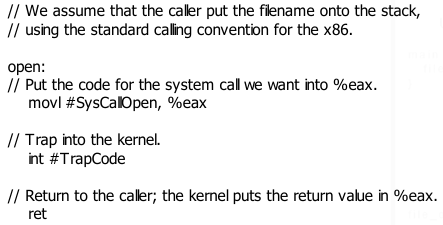
\includegraphics[scale=0.45]{img/fig11}}
\caption{\textit{Stub} de la biblioteca a nivel de usuario para el sistema de archivos de llamada al sistema abierto para el procesador x$86$. \textit{SysCallOpen} es el código de la llamada al sistema específico para funcionar. \textit{TrapCode} es el índice en la tabla de vectores de interrupción x$86$ para el controlador de llamada al sistema.}
\label{fig11}
\end{figure}

A continuación describimos estos pasos con más detalle. La \textit{fig} \ref{fig11} ilustra el comportamiento de la colilla a nivel de usuario para las arquitecturas x$86$. El sistema operativo proporciona una rutina de biblioteca para cada llamada al sistema que toma sus argumentos, les cambia el formato de acuerdo con la convención de llamada, y ejecuta una instrucción \textit{trap}. Cuando el núcleo devuelve, el stub devuelve el resultado proporcionado por el núcleo. Por supuesto, el programa de usuario no necesita utilizar la rutina de biblioteca -la \textit{trap} esta directamente en el núcleo; a su vez, el núcleo debe protegerse de los programas malisiosos que no formatean correctamente los argumentos.

La convención de llamada al sistema es arbitraria. En la \textit{fig} \ref{fig11}, el código pasa sus argumentos en la pila de usuario, almacenando el código de llamada del sistema en el registro $\% eax$. El valor de retorno regresa en $\% eax$, así que no hay trabajo que hacer en la vuelta.

La instrucción \textit{int} ahorra el contador de programa, puntero de pila, y \textit{eflags} en la pila del núcleo antes de saltar al controlador de llamada al sistema a través de la tabla vectorial de interrupción. El controlador del núcleo guarda todos los registros adicionales que deben ser preservados después de las llamadas a funciones. A continuación, examina el código entero de la  llamada al sistema en $\% eax$, verifica que se trata de un código de operación legal, y llama al código auxiliar correcto para esa llamada al sistema.

El \textit{stub} del núcleo tiene cuatro tareas:
\begin{itemize}
\item \textbf{Localiza argumentos de llamada del sistema.} A diferencia de un procedimiento normal del núcleo, los argumentos a una llamada de sistema se almacenan en la memoria de usuario, por lo general en la pila de usuario. Por supuesto, el puntero de pila de usuario puede estar dañado. Incluso si es válido, se trata de una dirección virtual, no una física. Si la llamada al sistema tiene un argumento de puntero (por ejemplo, un nombre de archivo), el \textit{stub} debe comprobar la dirección para verificar que es un domicilio legal dentro del dominio de usuario. Si es así, el \textit{stub} de la convierte a una dirección física de manera que el núcleo puede utilizar con seguridad. En la \textit{fig.} \ref{fig11} , el puntero a la cadena que representa el nombre del archivo se almacena en la pila; Por lo tanto, el talón debe revisar y traducir tanto la dirección de pila y el
puntero de cadena.
\item \textbf{Validar los parámetros.} El núcleo también debe protegerse contra los errores accidentales o maliciosos en el formato o el contenido de sus argumentos. Un nombre de archivo es típicamente una cadena terminada en cero, pero el núcleo no se puede confiar en el código de usuario trabaje siempre correctamente. El nombre de archivo puede estar dañado; se puede señalar a la memoria fuera de la región de la solicitud; puede comenzar dentro de la región de memoria de la aplicación sino que se extienden más allá de ella; la aplicación puede no tener permiso para acceder al archivo; puede no existir el archivo; Etcétera. Si se detecta un error, el núcleo devuelve al programa de usuario; de otro modo, el núcleo realiza la operación en nombre de la aplicación.

\item \textbf{Copiar antes de la llegada.} En la mayoría de los casos, los parámetros de llamada del sistema se copian en la memoria del kernel antes de realizar los controles necesarios. La razón de esto es evitar que la aplicación de la modificación del parámetro después del stub comprueba el valor, pero antes de que el parámetro se utiliza en la aplicación real de la rutina. Esto se llama un registro de entrada en función del tiempo de uso de ataque (TOCTOU). Por ejemplo, la aplicación podría llamar abierto con un nombre de archivo válido, pero, después de la verificación, cambiar el contenido de la cadena a ser un nombre diferente, como un archivo que contiene los datos privados de otro usuario.

TOCTOU no es un nuevo ataque - las primeras fechas de ocurrencia de los mediados de los años 1960 de. Aunque podría parecer que un proceso se detiene necesariamente cada vez que lo hace una llamada al sistema, esto no siempre es el caso. Por ejemplo, si un proceso comparte una región de memoria con otro proceso, entonces los dos procesos que trabajan juntos pueden lanzar un ataque TOCTOU. Del mismo modo, un programa que se ejecuta en paralelo dos procesadores puede lanzar un ataque TOCTOU, donde uno trampas procesador en el núcleo mientras que el otro modifica la cadena precisamente en la derecha (o mal) tiempo. Tenga en cuenta que el núcleo tiene que ser correcta en todos los casos, mientras que el atacante puede tratar de cualquier número de veces antes de tener éxito.

\item \textbf{Copiar de nuevo ningún resultado.} Para el programa de usuario para acceder a los resultados de la llamada al sistema, el talón debe copiar el resultado de la almendra en la memoria de usuario. Una vez más, el núcleo debe comprobar primero la useraddress y convertirla en una dirección del núcleo antes de realizar la copia.
\end{itemize}

\section{Inicio de un nuevo proceso}

Hasta el momento, hemos descrito cómo transferir el control de un proceso a nivel de usuario en una interrupción en el núcleo, a excepción del procesador, o llamada al sistema y cómo el núcleo reanuda la ejecución a nivel de usuario cuando haya terminado.

Examinaremos ahora cómo empezar a correr a nivel de usuario en primer lugar. El núcleo debe:
\begin{itemize}
\item Asignar e inicializar el bloque de control de proceso.
\item Asignar memoria para el proceso.
\item Copie el programa del disco a la memoria recién asignada.
\item Asignar una pila de nivel de usuario para su ejecución a nivel de usuario.
\item Asignar una pila a nivel de kernel para el manejo de llamadas del sistema, interrupciones y excepciones del procesador.
\end{itemize}

Para iniciar la ejecución del programa, el núcleo también debe:
\begin{itemize}
\item \textbf{Copiar argumentos en la memoria de usuario.} Al iniciar un programa, el usuario puede darle argumentos, tanto como llamar a un procedimiento. Por ejemplo, cuando se hace clic en un icono de archivo en MacOS o Windows, el gestor de ventanas pide al kernel para iniciar la aplicación asociada con el archivo, pasándole el nombre de archivo que desea abrir. El núcleo copia el nombre de archivo de la memoria del proceso gestor de ventanas a una región especial de memoria en el nuevo proceso. Por convención, los argumentos a un proceso se copian en la base de la pila a nivel de usuario, y el puntero de pila del usuario se incrementa por lo que esas direcciones no se sobrescriben cuando el programa se pone en marcha.

\item \textbf{Transferir el control a modo de usuario.} Cuando se inicia un nuevo proceso, no existe un estado guardada para restaurar. Aunque sería posible escribir código especial para este caso, la mayoría de los sistemas operativos de volver a utilizar el mismo código para salir del núcleo para iniciar un nuevo proceso y para el retorno de una llamada al sistema. Cuando creamos el nuevo proceso, asignamos una pila del núcleo a la misma, y nos reservamos habitación en la parte inferior de la pila del núcleo de los valores iniciales de sus registros de espacio de usuario, contador de programa, puntero de pila, y la palabra de estado del procesador. Para iniciar el nuevo programa, entonces podemos cambiar a la nueva pila y salta a la final del manejador de interrupciones. Cuando el controlador se ejecuta POPAD y iret, el procesador "devuelve" al inicio del programa de usuario.
\end{itemize}

Por último, aunque se puede pensar en un programa de usuario como a partir de una llamada a la principal, de hecho, el compilador inserta un nivel de indirección. Se pone un trozo en la ubicación en la memoria del proceso en el que el núcleo saltará cuando se inicia el proceso. El trabajo del talón es llamar principal y luego, si los retornos principales, para llamar a la salida - la llamada al sistema para terminar el proceso. Sin el talón, un programa de usuario que regresó de principal sería tratar de hacer estallar el contador de programa de retorno, y puesto que no hay tal dirección en la pila, la
procesador sería comenzar a ejecutar código aleatorio.

\chapter{La interfaz de programación}
En el capítulo anterior nos referimos a los mecanismos necesarios en el núcleo del sistema operativo para ejecutar el proceso de abstracción. Un proceso es una instancia de un programa - el kernel proporciona un recinto de seguridad eficiente para ejecutar código no confiable a nivel de usuario, se ejecuta código de usuario directamente en el procesador.

Este capítulo se refiere a cómo elegimos usar la abstracción de proceso: qué funcionalidad del sistema operativo proporciona aplicaciones, y donde deberían ir - qué la funcionalidad se debe poner en el núcleo del sistema operativo, lo que se debe poner en bibliotecas a nivel de usuario, y cómo debe organizarse el sistema operativo en sí mismo?

Hay tantas respuestas a estas preguntas como sistemas operativos existen. En este capítulo se explora un subconjunto de la interfaz de programación de UNIX, la base de Linux, MacOS, iOS y Android.

En primer lugar, tenemos que responder "qué" - ¿qué funciones qué necesitamos en un sistema operativo para proporcionar aplicaciones?
\begin{itemize}
\item \textbf{Gestión de proceso.} ¿Puede un programa crear una instancia de otro programa? Espere a que se complete? Detener o reanudar otro programa en ejecución? Envíar un evento asíncrono?

\item \textbf{De entrada y salida.} ¿Qué procesos se comunican con los dispositivos conectados al ordenador y a través de ellos con el mundo físico? ¿Pueden los procesos de comunicarse entre sí?

\item \textbf{Gestión de hilos.} ¿Podemos crear múltiples actividades o hilos que comparten memoria u otros recursos dentro de un proceso? ¿Podemos detener e iniciar las discusiones? ¿Cómo sincronizar su uso de estructuras de datos compartidos?

\item \textbf{Gestión de la memoria.} ¿Puede un proceso de pedir más (o menos) espacio de memoria? Puede compartir la misma región de memoria física con otros procesos?

\item \textbf{Sistemas de archivo y almacenamiento.} ¿Cómo funciona un proceso de almacenar los datos del usuario persistentemente para que pueda sobrevivir si la máquina se cuelga o si falla el disco? ¿De qué manera el nombre de usuario organiza sus datos?

\item \textbf{Redes y sistemas distribuidos.} ¿Qué procesos se comunican con los procesos de otros equipos? ¿De qué manera los procesos en diferentes equipos coordinan sus acciones a pesar de si la máquina se cuelga y hay problemas en la red?

\item \textbf{Los gráficos y la gestión de ventanas.} ¿Cómo funciona un píxel de control de procesos en su porción de la pantalla? ¿Cómo funciona un proceso para hacer uso de aceleradores gráficos?

\item \textbf{Autenticación y seguridad.} ¿Qué permisos tienen un usuario o un programa, y cómo estos permisos se mantienen hasta la fecha? ¿En base a qué sabemos que el usuario (o programa) es quien dice ser?
\end{itemize}

En este capítulo, nos centramos en sólo los dos primeros de estos temas: gestión de procesos y de entrada / salida. Podemos describir una interfaz funcional para la gestión de procesos y de entrada / salida con sólo una docena de llamadas al sistema, y el resto de la interfaz de llamada al sistema con otra docena. Más sorprendente aún, estas llamadas son casi sin cambios respecto al diseño original de UNIX. A pesar de estar diseñado e implementado en la década de 1970 en primer lugar, la mayoría de estas llamadas se encuentran todavía en amplio uso en los sistemas de hoy.

\begin{figure}[tbhp]
\centerline{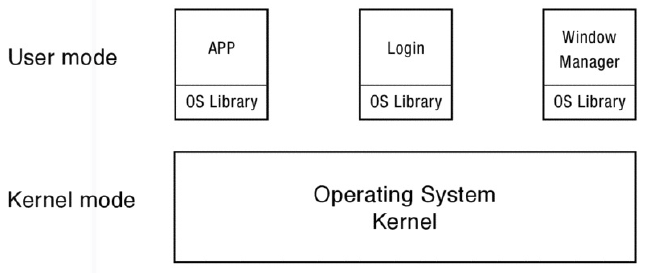
\includegraphics[scale=0.45]{img/fig12}}
\caption{La funcionalidad del sistema operativo puede ser implementada en programas a nivel de usuario, en las bibliotecas a nivel de usuario, en el propio núcleo, o en un servidor de nivel de usuario invocado por el núcleo.}
\label{fig12}
\end{figure}

En segundo lugar, tenemos que responder "donde" - para cualquier bit de funcionalidad del sistema operativo que proporciona a los programas de usuario, tenemos varias opciones para decidir donde vive, se ilustra en la \textit{fit.} \ref{fig12}:

\begin{itemize}
\item \textbf{Podemos poner la funcionalidad en un programa a nivel de usuario.} En Windows y UNIX, por ejemplo, hay un programa de usuario para la gestión de inicio de sesión de un usuario y otro para la gestión de los procesos de un usuario.

\item \textbf{Podemos poner la funcionalidad de una biblioteca a nivel de usuario vinculados con cada aplicación.} En Windows y MacOS, widgets de interfaz de usuario son parte de las bibliotecas a nivel de usuario, incluidas en aquellas aplicaciones que lo necesiten.

\item \textbf{Podemos poner la funcionalidad en el núcleo del sistema operativo, se accede a través de una llamada al sistema.} En Windows y UNIX, la gestión de procesos de bajo nivel, el sistema de archivos y la pila de red se implementan en el núcleo.

\item \textbf{Podemos acceder a la función a través de una llamada al sistema, pero implementar la función en un proceso de servidor autónomo invocado por el núcleo.} En muchos sistemas, el gestor de ventanas se implementa como un proceso de servidor independiente.
\end{itemize}

¿Cómo podemos hacer esta elección? Es importante darse cuenta de que la elección puede ser (en su mayoría) transparente tanto para el usuario y el programador de la aplicación. El usuario quiere un sistema que funciona; el programador quiere una interfaz limpia y cómoda que hace el trabajo. Mientras el sistema operativo proporciona la interfaz, donde cada función se implementa es de hasta el sistema operativo, en base a un compromiso entre la \textit{flexibilidad}, \textit{fiabilidad}, \textit{rendimiento} y \textit{seguridad}.

\begin{itemize}
\item \textbf{Flexibilidad.} Es mucho más fácil cambiar el código del sistema operativo que vive fuera del núcleo, sin romper las aplicaciones utilizando la interfaz de edad. Si creamos una nueva versión de una biblioteca, sólo podemos vincular esa biblioteca con nuevas aplicaciones, y con el tiempo convertir las aplicaciones antiguas para utilizar la nueva interfaz. Sin embargo, si hay que cambiar la interfaz de llamada al sistema, debemos o bien cambiar al mismo tiempo tanto el núcleo como todas las aplicaciones, o debemos seguir apoyando a las versiones de la antigua y de la nueva hasta que todas las aplicaciones antiguas han sido convertidos. Muchas aplicaciones son escritas por desarrolladores de terceras partes, fuera del control del proveedor del sistema operativo. Por lo tanto, el cambio de la interfaz de llamada al sistema es un gran paso, que a menudo requiere la coordinación a través de muchos
compañías.

\item \textbf{Seguridad.} Sin embargo, la gestión y protección de los recursos son responsabilidad del núcleo del sistema operativo. Como explicó el capítulo 2, los controles de protección no se pueden implementar en una biblioteca de nivel de usuario porque el código de aplicación puede saltarse todas las comprobaciones realizadas por la biblioteca.

\item \textbf{Confiabilidad.} Mejora de la fiabilidad es otra razón para mantener el núcleo del sistema operativo mínimo. código del kernel necesita el poder para configurar los dispositivos de hardware, tales como el disco, y para controlar los límites de protección entre aplicaciones. Sin embargo, los módulos del núcleo en general no son protegidos de los otros, y por lo que un error en el código del kernel (ya sea sensible o no) puede destruir los datos de usuario o kernel. Esto ha llevado a algunos sistemas de utilizar una filosofía de "lo que puede ser a nivel de usuario, que debe ser." Una versión extrema de enfoque consiste en aislar privilegiada, pero menos crítica, partes del sistema operativo, como el sistema de archivos o el sistema de ventanas , desde el resto del núcleo. Esto se llama un diseño de microkernel. En un microkernel, el propio núcleo se mantiene pequeño, y en su lugar la mayor parte de la funcionalidad de un núcleo de sistema operativo tradicional se pone en un conjunto de nivel de usuario
procesos, o servidores, se accede desde las aplicaciones de usuario a través de a comunicación entre procesos.

\item \textbf{Rendimieno.} Finalmente, la transferencia de control en el núcleo es más caro que una llamada de procedimiento a una biblioteca, y transferir el control a un servidor de sistema de archivos de nivel de usuario a través del núcleo es todavía aún más costoso. diseñadores de hardware han tratado de reducir el costo de estos cruces de límites, pero su rendimiento sigue siendo un problema. Microsoft Windows NT, un precursor de Windows 7, se diseñó inicialmente como un microkernel, pero con el tiempo, gran parte de su funcionalidad se ha migrado hacia atrás en el núcleo por razones de rendimiento.
\end{itemize}

\section{Gestión de Procesos}
En un equipo moderno, cuando un usuario hace clic en un icono de archivo o una aplicación, la aplicación se inicia. ¿Cómo sucede esto y quien es llamado? Por supuesto, podríamos poner en práctica todo lo que tiene que ocurrir en el kernel - dibujar el icono para cada elemento en el sistema de archivos, las posiciones que marca el ratón sobre el icono deseado, coger el clic del ratón, y comienzan el proceso. En los sistemas de procesamiento por lotes tempranos, el núcleo estaba en control por necesidad. Usuarios presentaron puestos de trabajo, y el sistema operativo toma a partir de ahí, una instancia del proceso cuando llega el momento de ejecutar el trabajo.

Un enfoque diferente es permitir que los programas de usuario puedan crear y gestionar sus propios procesos. Esto ha fomentado una tormenta de nieve de la innovación. Hoy en día, los programas que crean y gestionan procesos incluyen los gestores de ventanas, servidores web, los navegadores web, intérpretes de línea de comandos \textit{shell}, sistemas de control de código fuente, bases de datos, compiladores y sistemas de preparación de documentos, etc. Si la creación de un proceso es algo que un proceso puede hacer, entonces cualquiera puede construir una nueva versión de cualquiera de estas aplicaciones, sin tener que recompilar el kernel o forzar a nadie a usarlo.

Una motivación temprana para la gestión de procesos a nivel de usuario era permitir a los desarrolladores escribir sus propios intérpretes de línea de comandos \textit{shell}. Una \textit{shell} es un sistema de control de trabajo; Windows y UNIX tienen una. Muchas tareas implican una secuencia de pasos para hacer algo, cada uno de los cuales puede ser su propio programa. Con una \textit{shell}, se puede escribir la secuencia de pasos, como una secuencia de programas a ejecutar para hacer cada paso. Por lo tanto, se puede ver como una versión muy temprana de un sistema de scripting.

\subsection{Gestión de Procesos de Windows}
Un enfoque para la gestión de procesos es simplemente agregar una llamada al sistema para crear un proceso y otro sistema de llamadas para otras operaciones de proceso. Esta resulta ser simple en teoría y compleja en la práctica. En Windows, hay una rutina llamada, como era de esperar, \textit{CreateProcess}.

Nosotros llamamos al creador de procesos ''proceso padre'' y a los creados, ''procesos hijos''. ¿Qué pasos toma CreateProcess? Como ya hemos explicado en el capítulo anterior, el núcleo necesita:

\begin{itemize}
\item Crear e inicializar el bloque de control de proceso (PCB) en el núcleo.
\item Crear e inicializar un nuevo espacio de direcciones.
\item Cargar el programa progresivo en el espacio de direcciones.
\item Copiar los argumentos args en la memoria en el espacio de direcciones.
\item Inicializar el contexto de hardware para comenzar la ejecución en "start".
\item Informar al programador que el nuevo proceso está listo para funcionar.
\end{itemize}

Por desgracia, hay un buen número de aspectos del proceso padre que pueda querer controlar, tales como: sus privilegios, donde envía su entrada y salida, lo que debería almacenar en sus archivos, lo que usa como prioridad de planificación, y demas. No podemos confiar en el proceso hijo para establecer sus propios privilegios y prioridad, y sería un inconveniente esperar cada solicitud de inclusión de código para averiguar su contexto. Por lo tanto la interfaz real para \textit{CreateProcess} es un poco más complicada en la práctica.

\subsection{Gestión de Procesos de UNIX}
UNIX tiene un enfoque diferente para el manejo de procesos, que es complejo en la teoría y simple en la práctica. UNIX divide en dos etapas a CreateProcess, llamadas \textit{fork} y \textit{exec}, que se ilustra en la \textit{fig.} \ref{fig13}:
\begin{figure}[tbhp]
\centerline{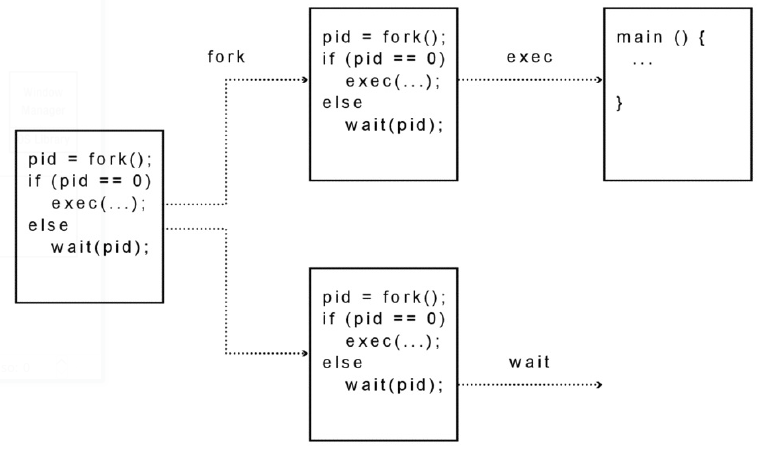
\includegraphics[scale=0.45]{img/fig13}}
\caption{El funcionamiento de las llamadas \textit{fork()} y \textit{exec()}. \textit{fork()} hace una copia del proceso padre; UNIX \textit{exec()} cambia el proceso hijo para ejecutar el nuevo programa.}
\label{fig13}
\end{figure}

UNIX \textit{fork} crea una copia completa del proceso padre, con una excepción clave. (Necesitamos una manera de distinguir entre el padre y la copia del mismo, el hijo.) El proceso hijo establece privilegios, prioridades, y E/S para el programa que está a punto de comenzar, por ejemplo, mediante el cierre de algunos archivos, la apertura de los demás, lo que reduce su prioridad si se va a ejecutar en segundo plano, etc. Debido a que el hijo corre exactamente el mismo código que el padre, se puede confiar en que va a establecer el contexto para el nuevo programa correctamente.

Una vez que se establece el contexto, el proceso hijo llama UNIX \textit{exec}. UNIX exec trae la nueva imagen ejecutable en la memoria y lo pone en marcha. Puede parecer un desperdicio hacer una copia completa del proceso padre, sólo para sobrescribir esa copia cuando traemos en la nueva imagen ejecutable en la memoria usando exec. Resulta que fork y exec se pueden implementar de manera eficiente, utilizando una serie de técnicas que describiremos en el capítulo 8.

Con este diseño, UNIX fork no tiene argumentos y devuelve un entero. UNIX exec toma dos argumentos (el nombre del programa a ejecutar y una serie de argumentos para transmitir al programa). Esto es, en lugar de los diez parámetros necesarios para CreateProcess. En parte debido a la simplicidad de fork y exec, esta interfaz se ha mantenido prácticamente sin cambios desde que UNIX fue diseñado en la década de los $70$. (Aunque la interfaz no ha cambiado, la palabra fork es ahora un poco ambigua. Se utiliza para crear una nueva copia de un proceso, y en sistemas de hilos para crear un nuevo hilo. Para eliminar la ambigüedad, siempre vamos a utilizar el término ''UNIX fork'' para referirse a la llamada al sistema de proceso de copia de UNIX).

\setlength{\parindent}{20pt} \textbf{Unix fork} \setlength{\parindent}{0pt}

Los pasos para la implementación de frok en el núcleo son:
\begin{itemize}
\item Crear e inicializar el bloque de control de proceso (PCB) en el núcleo
\item Crear un nuevo espacio de direcciones
\item Inicializar el espacio de direcciones con una copia de todo el contenido del espacio de direcciones de la matriz
\item Heredar el contexto de ejecución de los padres (por ejemplo, todos los archivos abiertos)
\item Informar al programador que el nuevo proceso está listo para funcionar
\end{itemize}

Un aspecto extraño del fork es que la llamada al sistema devuelve dos valores: uno para el padre y uno para el hijo. Para los padres, UNIX devuelve el ID del proceso hijo; para el hijo, devuelve cero que indica el éxito. Del mismo modo que si ha cometido un clon de sí mismo, lo que se necesita es alguna forma de saber quién era el clon y quien era el original, UNIX utiliza el valor de retorno de fork para distinguir las dos copias.

\setlength{\parindent}{20pt} \textbf{UNIX exec y wait} \setlength{\parindent}{0pt}

La llamada al sistema exec completa los pasos necesarios para iniciar la ejecución de un nuevo programa. El proceso hijo llama normalmente a exec una vez que ha regresado del fork y configurado el entorno de ejecución para el nuevo proceso. Exec realiza los siguientes pasos (tenga en cuenta que exec no crea un nuevo proceso):
\begin{itemize}
\item Cargar el programa progresivo en el espacio de direcciones actual.
\item Copia los argumentos args en la memoria en el espacio de direcciones.
\item Inicializar el contexto de hardware para comenzar la ejecución en "inicio".
\end{itemize}

En el otro lado, a menudo el proceso padre necesita hacer una pausa hasta que el proceso hijo haya termiando, por ejemplo, si el siguiente paso depende de la salida de la etapa anterior. UNIX tiene una llamada al sistema, como es natural llamada \textit{wait}, que detiene a los padre hasta que el hijo termina, se bloquea o se termina. Dado que el padre podría haber creado muchos procesos hijos, wait ha parametrizado con el ID de proceso del hijo.

Por último, como hemos descrito en el capítulo anterior, UNIX proporciona la posibilidad de que un proceso pueda mandar a otro proceso una notificación instantánea o llamada ascendente. En UNIX, la notificación se envía enviando una \textit{signal}. Las señales se utilizan para la terminación de una aplicación, se suspende temporalmente para la depuración, la reanudación después de una suspensión, expiración del temporizador, y una serie de otras razones. Por lo general, si la aplicación receptora no especificó un manejador de señales, el núcleo implementa una estándar en su nombre.

\section{Estructura del Sistema Operativo}
Empezamos este capítulo con una lista de funcionalidades que los usuarios y las aplicaciones necesitan desde el sistema operativo. Hemos demostrado que mediante un cuidadoso diseño de la interfaz de llamadas al sistema, podemos descargar parte de la labor del sistema operativo para los programas de usuario, como por ejemplo una \textit{shell} o un servidor de impresión.

En el resto de este capítulo, nos preguntamos ¿cómo debemos organizar las partes restantes del sistema operativo?. Hay muchas dependencias entre los módulos dentro del sistema operativo, y no hay interacción a menudo bastante frecuente entre estos módulos:

\begin{itemize}
\item Muchas partes del sistema operativo dependen de primitivas de sincronización para coordinar el acceso a las estructuras de datos compartidos con el kernel.
\item El sistema de memoria virtual depende del soporte de hardware de bajo nivel para la traducción de direcciones, un apoyo que es específico para una arquitectura de procesador en particular.
\item Tanto el sistema de archivos y el sistema de memoria virtual comparten una base común de bloques de memoria física. Ambos también dependen del controlador de dispositivo de disco.
\item El sistema de archivos puede depender de la pila de protocolos de red si el disco se encuentra físicamente en un equipo diferente.
\end{itemize}

Esto ha llevado a los diseñadores del sistema operativo a luchar con un compromiso fundamental: mediante la centralización de funciones en el kernel, se mejora el rendimiento y hace que sea más fácil de organizar una estrecha integración entre los módulos del núcleo. Sin embargo, los sistemas resultantes son menos flexibles, menos fáciles de cambiar, y menos adaptables a las necesidades del usuario de aplicación. Se discuten estos intercambios mediante la descripción de varias opciones para la arquitectura del sistema operativo.

\subsection{Núcleos monolíticos}
\begin{figure}[tbhp]
\centerline{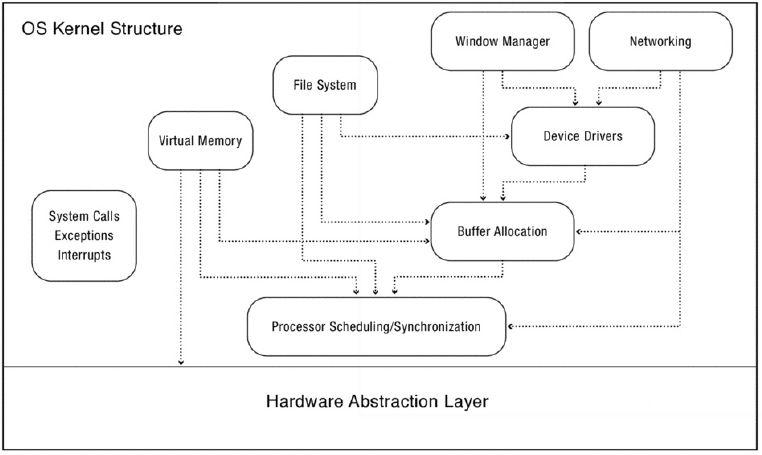
\includegraphics[scale=0.45]{img/fig14}}
\caption{En un núcleo de sistema operativo monolítico, la mayor parte de la funcionalidad del sistema operativo está relacionado entre sí dentro del núcleo. Los módulos del kernel llaman directamente a otros módulos del kernel para realizar las funciones necesarias. Por ejemplo, el sistema de memoria virtual utiliza gestión de memoria intermedia, la sincronización, y la capa de abstracción de hardware.}
\label{fig14}
\end{figure}

Casi todos sistemas operativos comerciales ampliamente utilizados, como Windows, MacOS y Linux, pueden adoptar un enfoque similar a la arquitectura del núcleo - un diseño monolítico. Como se muestra en la \textit{fig.} \ref{fig14}, con un núcleo monolítico, la mayor parte de la funcionalidad del sistema operativo funciona en el interior del núcleo del sistema operativo. En verdad, el término es un nombre poco apropiado, porque incluso en los llamados sistemas monolíticos, a menudo hay grandes segmentos de lo que los usuarios consideran que el sistema operativo se ejecuta fuera del núcleo, ya sea como empresas de servicios públicos como la shell, o en las bibliotecas del sistema, tales como bibliotecas para gestionar la interfaz de usuario.

Interno a un núcleo monolítico, el diseñador del sistema operativo es libre de desarrollar cualesquiera que sean las interfaces entre los módulos que tienen sentido, y por lo que hay un poco de variación de un sistema operativo a otro en esas estructuras internas. Sin embargo, dos temas comunes en todos los sistemas son: para mejorar la portabilidad, casi todos los sistemas operativos modernos tienen tanto una capa de abstracción de hardware y controladores de dispositivos de carga dinámica.

\setlength{\parindent}{20pt} \textbf{Capa de Abstracción de Hardware} \setlength{\parindent}{0pt}

Un objetivo clave de los sistemas operativos es ser portable a través de una amplia variedad de plataformas de hardware. Para lograr esto, especialmente dentro de un sistema monolítico, se requiere un diseño cuidadoso de la capa de abstracción de hardware. La capa de abstracción de hardware \textit{(HAL)} es una interfaz portátil de configuración de la máquina y operaciones específicas del procesador dentro del kernel. Por ejemplo, dentro de la misma familia de procesadores, tales como Intel x$86$, diferentes fabricantes de ordenadores requerirán un código específico diferente del equipo para configurar y gestionar las interrupciones y temporizadores de hardware.

Los sistemas operativos que pueden llevarse a distintas familias de procesadores, es decir entre un ARM y un sistema x$86$ o entre una de $32$ bits y un x$86$ de $64$ bits, necesitará el código específico del procesador de interruptores de proceso e hilos. La manipulación de la \textit{trap} de interrupción, a excepción del procesador y la llamada al sistema es también específico del procesador; todos los sistemas tienen estas funciones, pero la aplicación concreta puede variar. Como veremos en el capítulo 8, máquinas difieren un poco en su arquitectura para la gestión de espacios de direcciones virtuales; la mayoría de los kernels proporcionan abstracciones portátiles en la parte superior de las rutinas dependientes de la máquina, como para traducir direcciones virtuales a direcciones físicas o copiar de la memoria de aplicaciones a la memoria del núcleo y viceversa.

Con una capa de abstracción de hardware bien definida en su lugar, la mayor parte del sistema operativo es una máquina ya independiente del procesador. Por lo tanto, portar un sistema operativo para un nuevo ordenador es sólo una cuestión de crear nuevas implementaciones de estas rutinas de bajo nivel HAL y re-vinculación.

\setlength{\parindent}{20pt} \textbf{Instalando dinámicamente los controladores de dispositivos} \setlength{\parindent}{0pt}

Una consideración similar conduce a sistemas operativos que pueden acomodar fácilmente una amplia variedad de dispositivos de E/S. Aunque hay sólo un puñado de diferentes arquitecturas de conjuntos de instrucciones de uso generalizado hoy en día, hay un gran número de diferentes tipos de dispositivos de E/S, fabricados por un gran número de empresas. Existe diversidad en las interfaces de hardware en los dispositivos, así como en los conjuntos de chips de hardware para la gestión de los dispositivos.

Para mantener la portabilidad del núcleo del sistema operativo, queremos desacoplar el código fuente del sistema operativo de los aspectos específicos de cada dispositivo. Por ejemplo, supongamos que un fabricante crea una nueva impresora - ¿qué medidas necesita tomar el fabricante del sistema operativo para dar cabida a ese cambio?

La innovación clave, ampliamente adoptada hoy, es un controlador de dispositivo de carga dinámica. Un controlador de dispositivo de carga dinámica es un software para gestionar un dispositivo específico, interfaz o conjunto de chips, agregado al núcleo del sistema operativo después de que el núcleo comienza a funcionar, para manejar los dispositivos que están presentes en una máquina en particular. El fabricante del dispositivo normalmente proporciona el código del controlador, utilizando una interfaz estándar soportado por el núcleo. El núcleo del sistema operativo llama al controlador cada vez que necesita para leer o escribir datos en el dispositivo.

El sistema operativo con un pequeño número de controladores de dispositivos - por ejemplo, para el disco (para leer el binario sistema operativo en la memoria). Para los dispositivos conectados físicamente al equipo, el fabricante del equipo reúne los conductores en un archivo que almacena junto con el gestor de arranque. Cuando el sistema operativo se inicia, consulta el bus de E/S para los dispositivos que están conectados a la computadora y luego carga los controladores del archivo en el disco. Por último, para cualquier dispositivo conectado a la red, tal como una impresora de red, el sistema operativo puede cargar los conductores a través de Internet.

Mientras que los controladores de dispositivo se pueden cargar dinámicamente para resolver un problema, suponen uno diferente. Los errores en un controlador de dispositivo pueden corromper las estructuras del kernel del sistema operativo y datos de aplicación; al igual que con un programa regular, los errores no pueden ser capturados de inmediato, de modo que el usuario puede no ser consciente de que sus datos están siendo modificados en silencio. Lo que es peor, un atacante malintencionado puede utilizar controladores de dispositivo para introducir un virus informático en el núcleo del sistema operativo, y por lo tanto obtener el control de todo el equipo.

Los desarrolladores de sistemas operativos han llevado a cabo cinco enfoques para hacer frente a este problema:

\begin{itemize}
\item \textbf{Inspección de código.} proveedores de sistemas operativos suelen requerir todo el código de controlador de dispositivo que se presente antes que las inspecciones y pruebas, antes de introducirse en el núcleo.

\item \textbf{El seguimiento de errores.} Después de cada caída del sistema, el sistema operativo puede recopilar información acerca de la configuración del sistema y de la pila del núcleo actual, y envía esta información a una base de datos central para su análisis. Microsoft hace esto en una escala amplia. Con cientos de millones de ordenadores instalados, incluso una baja tasa de fracaso puede producir millones de informes de errores por día. Muchos accidentes ocurren dentro del controlador de dispositivo en sí, pero incluso aquellos que no lo hacen a veces pueden ser localizados. Por ejemplo, si los fallos se correlacionan con la presencia de un controlador de dispositivo en particular, o aumento después del lanzamiento de una nueva versión del controlador, que puede indicar el origen de un problema.

\item \textbf{Controladores de dispositivos a nivel de usuario.} Tanto Apple como Microsoft estimulan fuertemente nuevos controladores de dispositivos para funcionar a nivel de usuario en lugar de en el núcleo. Cada controlador de dispositivo se ejecuta en un proceso independiente a nivel de usuario, mediante llamadas al sistema para manipular el dispositivo físico. De esta manera, un driver sólo puede afectar a sus propias estructuras de datos internos y no el resto del núcleo del sistema operativo; si el controlador de dispositivo se bloquea, el núcleo puede reiniciar fácilmente.

A pesar de que los controladores de dispositivos a nivel de usuario son cada vez más comunes, puede llevar mucho tiempo a los controladores de dispositivos existentes en el puerto ejecutar a nivel de usuario. Por desgracia, hay una enorme cantidad de código de controlador de dispositivo que se dirige directamente a las estructuras de datos del núcleo interno existente; trazando una frontera en torno a estos controladores ha demostrado ser difícil. Por supuesto, el apoyo a los conductores de legado es un problema menor como completamente nuevas plataformas de hardware y sistemas operativos, tales como teléfonos inteligentes y tabletas, se desarrolló.

\item \textbf{Controladores de dispositivo de la máquina virtual.} Para manejar los controladores de dispositivos de legado, un enfoque que ha ganado algo de tracción es ejecutar el código del controlador de dispositivo dentro de un sistema operativo invitado que se ejecuta en una máquina virtual. El sistema operativo invitado carga los controladores de dispositivo como si se estaba ejecutando directamente en el hardware real, pero cuando los dispositivos intentan acceder al hardware físico, el monitor de máquina virtual subyacente recupera el control para garantizar la seguridad. Los controladores de dispositivos todavía pueden tener errores, pero sólo pueden dañar el sistema operativo invitado y no otras aplicaciones que se ejecutan en el monitor de máquina virtual subyacente.

\item \textbf{Controlador Sanboxing.} Otro desafío para ambos controladores de dispositivos a nivel de usuario y los controladores de la máquina virtual es el rendimiento. Algunos controladores de dispositivos necesitan una interacción frecuente con el hardware y el resto del núcleo. Algunos investigadores han propuesto ejecutar los controladores de dispositivo en su propio entorno de ejecución restringido en el interior del núcleo. Esto requiere técnicas sandboxing ligeros.
\end{itemize}

\subsection{MicroKernels}
Una alternativa al enfoque núcleo monolítico es ejecutar tanto del sistema operativo como sea posible en uno o más servidores de nivel de usuario. El gestor de ventanas en la mayoría de los sistemas operativos funciona de esta manera: aplicaciones individuales dibujan cosas en su porción de la pantalla mediante el envío de peticiones al gestor de ventanas. El gestor de ventanas, que adjudica ventana de aplicación está delante o detrás de cada píxel en la pantalla, y luego hace que el resultado. Si el sistema tiene un acelerador de gráficos de hardware
Actualmente, el gestor de ventanas puede utilizarlo para hacer que los artículos más rápidamente. Algunos sistemas han movido otras partes del sistema operativo en los servidores de nivel de usuario: la pila de red, el sistema de archivos, controladores de dispositivos, y así sucesivamente.

La diferencia entre un diseño de un microkernel monolítico y con frecuencia es transparente para el programador de la aplicación. La ubicación del servicio puede estar oculto en una biblioteca de nivel de usuario - llamadas van a la biblioteca, lo que arroja las solicitudes ya sea como llamadas al sistema o como leer y escribir en el servidor a través de una tubería. La ubicación del servidor también se puede ocultar en el interior del núcleo - la aplicación llama al núcleo como si el núcleo implementa el servicio, pero en su lugar el núcleo cambia el formato de la solicitud en una tubería que el servidor puede leer.

Un diseño de microkernel ofrece un beneficio considerable para el desarrollador del sistema operativo, ya que más fácil de modularizar y los servicios de depuración a nivel de usuario que el código del kernel. Aparte de un potencial de mejora de la fiabilidad, sin embargo, los micronúcleos ofrecen poco en el camino de beneficio visible a los usuarios finales y puede ralentizar el rendimiento general mediante la inserción de pasos adicionales entre la aplicación y los servicios que necesita. Por lo tanto, en la práctica, la mayoría de los sistemas de adoptar un modelo híbrido en el que algunos servicios del sistema operativo se ejecutan a nivel de usuario y algunos están en el núcleo, en función de la solución de compromiso entre la complejidad del código específico y el rendimiento.

\chapter{Concurrencia e Hilos}
En el mundo real - fuera de las computadoras - diferentes actividades con frecuencia ocurren al mismo tiempo. Usamos la palabra \textit{Concurrencia} para referirnos a múltiples actividades que pueden ocurrir al mismo tiempo. El mundo real es concurrente, e internamente, las computadoras modernas también son concurrentes. Por ejemplo, un servidor de gama alta puede tener más de una docena de procesadores, discos, $10$ y $4$ interfaces de red; una estación de trabajo podría tener una docena de dispositivos de E/S activos que incluyen una pantalla, teclado, ratón, cámara, micrófono, altavoz, interfaz de red inalámbrica, cable de interfaz de red, una impresora, un escáner, y la unidad de disco. Hoy en día, incluso los teléfonos móviles suelen tener procesadores de múltiples núcleos.

La correcta gestión de la concurrencia es un desafío clave para los desarrolladores de sistemas operativos. Para gestionar los recursos de hardware, para proporcionar la capacidad de respuesta a los usuarios, y para ejecutar varias aplicaciones al mismo tiempo, el sistema operativo necesita una forma estructurada de hacer el seguimiento de las diversas acciones que necesita realizar. En los próximos capítulos, vamos a presentar un conjunto de abstracciones para expresar y gestionar la concurrencia. Estas abstracciones son de uso generalizado en los sistemas operativos comerciales, ya que reducen la complejidad de implementación, mejoran la fiabilidad del sistema y mejoran el rendimiento.

Concurrencia también es una preocupación para muchos desarrolladores de aplicaciones. A pesar de las abstracciones que discutimos fueron desarrollados originalmente para que sea más fácil escribir código del sistema operativo correcto, que han llegado a ser ampliamente utilizado en aplicaciones:
\begin{itemize}
\item Los servicios de red necesitan ser capaces de manejar múltiples peticiones de sus clientes; Google podría manejar sólo una solicitud de búsqueda a la vez, o Amazon sólo podría permitir un libro que se compra a la vez, sería mucho menos útil.
\item La mayoría de las aplicaciones de hoy en día tienen interfaces de usuario; proporcionar una buena capacidad de respuesta a los usuarios, realizando al mismo tiempo la lógica de aplicación es mucho más fácil con un enfoque estructurado para la concurrencia.
\item Programas paralelos tienen que ser capaces de cartografiar el trabajo en múltiples procesadores para obtener los beneficios de rendimiento de las arquitecturas multinúcleo.
\item Sistemas de gestión de datos necesitan de la concurrencia para enmascarar la latencia de las operaciones de disco y de red.
\end{itemize}

Desde la perspectiva del programador, es mucho más fácil pensar que secuencialmente para realizar un seguimiento de las muchas actividades simultáneas. Por ejemplo, al leer o escribir el código de un procedimiento, puede identificar un estado inicial y un conjunto de condiciones previas, pensar en cómo cada declaración sucesiva cambia el estado, y desde ese determinar las post-condiciones. ¿Cómo se puede escribir un programa correcto con docenas de eventos sucediendo al mismo tiempo? 

El sistema operativo proporciona la ilusión de que los programadores pueden crear tantos hilos, como necesiten, y cada hilo se ejecuta en su propio procesador virtual dedicado. En realidad, por supuesto, una máquina sólo tiene un número finito de procesadores, y es el trabajo del sistema operativo, de forma transparente, hacer hilos multiples en los procesadores actuales.

La idea clave es escribir un programa simultáneo - uno con muchas actividades simultáneas - como un conjunto de flujos secuenciales de ejecución, o hilos, que interactúan y comparten los resultados de maneras muy precisas. Definamos un conjunto de tareas que se ejecutan concurrentemente mientras que el código para cada tarea es secuencial. Cada hilo se comporta como si tuviera su propio procesador dedicado. Como veremos más adelante, utilizando la abstracción de hilo a menudo requiere que el programador escriba código adicional para la coordinación de múltiples hilos con el acceso a estructuras de datos compartidos.

La abstracción de hilo permite al programador crear tantos procesos como sea necesario, sin tener que preocuparse por el número exacto de procesadores físicos, o exactamente qué procesador va a trabajar en cada instante. Por supuesto, los hilos son solamente una abstracción: el hardware físico tiene un número limitado de procesadores (y potencialmente único). El trabajo del sistema operativo es el de proporcionar la ilusión de un número casi infinito de procesadores virtuales, incluso mientras el hardware físico es más limitado. Se sostiene esta ilusión mediante la suspensión y reanudación de hilos de modo que en cualquier momento dado sólo un subconjunto de los hilos se estén ejecutando activamente de manera transparente.

En este capítulo se definirá la abstracción hilo, se ilustra cómo un programador puede utilizar dicha abstracción, y se explica cómo el sistema operativo puede implementar los hilos en la parte superior de un número limitado de procesadores.

\section{Casos de uso de los Hilos}
La intuición detrás de la abstracción de hilo es simple: en un programa, podemos representar cada tarea concurrente como un hilo. Cada hilo proporciona la abstracción de ejecución secuencial similar al modelo de programación tradicional. De hecho, podemos pensar en un programa tradicional como un único subproceso con una secuencia lógica de pasos que cada instrucción sigue a la anterior. El programa ejecuta sentencias, itera a través de bucles y llamadas/retornos de procedimientos, uno tras otro.

Un programa multi-hilo es una generalización del mismo modelo de programación básica. A cada hilo individual le sigue una secuencia de pasos que ejecuta sentencias, itera a través de bucles, llamadas/retornos de procedimientos, etc. Sin embargo, un programa puede disponer de varias hilos que se ejecutan al mismo tiempo.

¿Cuándo es apropiado utilizar múltiples hilos dentro del mismo programa? Las discusiones han llegado a ser ampliamente utilizadas tanto en el código del sistema operativo como en la aplicación, y en base a esa experiencia, podemos identificar varios temas comunes.

\subsection{Cuatro razones para usar Hilos}
El uso de hilos para expresar y gestionar la concurrencia tiene varias ventajas:
\begin{itemize}
\item \textbf{Estructura del programa: expresar lógicamente tareas concurrentes.} Los programas a menudo interactúan o simulan aplicaciones del mundo real que tienen actividades concurrentes. Los hilos le permiten expresar concurrencia natural de una aplicación escribiendo cada tarea concurrente como un hilo separado. En la aplicación GPS, los hilos permiten que diferentes actividades - la actualización de la pantalla, ir a buscar datos adicionales, y recibir nuevas entradas de usuario - se ejecuten al mismo tiempo. Por ejemplo, para obtener la entrada del ratón y al mismo tiempo volver a dibujar la pantalla y enviar y recibir paquetes desde la red, los procesadores físicos tienen que dividir su tiempo entre estas tareas.

\item \textbf{Capacidad de respuesta: el cambio de trabajo se ejecuta en segundo plano.} Para mejorar la respuesta al usuario y el rendimiento, un patrón de diseño común es crear hilos para realizar un trabajo en segundo plano, sin que el usuario este esperando el resultado. De esta manera, la interfaz de usuario puede permanecer sensible a otros comandos, independientemente de la complejidad de la petición del usuario. En un navegador web, por ejemplo, el botón de cancelación debe continuar trabajando incluso si la página es gigantesca o una secuencia de comandos en la página tarda mucho tiempo para ejecutarse.

¿Como funciona esto? Muchas aplicaciones tienen un bucle: obtener una orden del usuario, a continuación, ejecutar el comando, a continuación, obtener el siguiente comando. Si algunos comandos toman mucho tiempo para llevarse a cabo, sin embargo, una aplicación que se ejecuta secuencialmente no será capaz de comprobar para la siguiente operación hasta que el anterior este completa. Para mantener la interfaz de respuesta, podemos utilizar hilos para dividir cada comando en dos partes: cualquier cosa que se puede hacer al instante se puede hacer en el bucle de eventos principal, y en un hilo separado podemos realizar el resto de la tarea en segundo plano. En el ejemplo del GPS, utilizamos hilos para mover las partes difíciles computacionalmente de la lógica de la aplicación - representación de la pantalla - fuera del circuito principal.

\item \textbf{Rendimiento: aprovecha múltiples procesadores.} Los programas pueden utilizar hilos en un multiprocesador que hace el trabajo en paralelo; pueden hacer el mismo trabajo en menos tiempo o más trabajo en el mismo tiempo transcurrido. Hoy en día, un servidor puede tener más de una docena de procesadores; una computadora de escritorio o portátil pueden incluir ocho núcleos de procesador; incluso la mayoría de los teléfonos inteligentes son máquinas multinúcleo. De cara al futuro, la ley de Moore hace que sea probable que el número de procesadores por sistema seguirá aumentando. Una ventaja de utilizar hilos para el paralelismo es que el número de hilos no tiene por qué coincidir exactamente con el número de procesadores en el hardware en el que se está ejecutando. El sistema operativo de maenera ransparente maneja los interruptores que ejecutan las discusiones sobre los procesadores.

\item \textbf{Rendimiento: gestión de los dispositivos de E/S.} Para hacer un trabajo útil, los equipos deben interactuar con el mundo exterior a través de los dispositivos de E/S. Mediante la ejecución de tareas como hilos separados, cuando una tarea está a la espera de E/S, el procesador puede avanzar en una tarea diferente.

El beneficio de la concurrencia entre el procesador y la E/S es doble: en primer lugar, los procesadores son a menudo mucho más rápido que los sistemas de E / S con las que interactúan, por lo que mantener la inactividad del procesador durante la I/O perdería gran parte de su capacidad . Por ejemplo, la latencia para leer desde el disco puede ser de decenas de milisegundos, lo suficiente para ejecutar más de 10 millones de instrucciones en un procesador moderno. Después de solicitar un bloque de disco, el sistema operativo puede cambiar a otro programa, o de otro hilo dentro del mismo programa, hasta que el disco haya finalizado y el hilo original está listo para reanudar.

En segundo lugar, E/S proporciona una forma para que la computadora para interactuar con entidades externas, como los usuarios presionar las teclas de un teclado o un equipo remoto que envía paquetes de red. La llegada de este tipo de eventos de E/S es impredecible, por lo que el procesador debe ser capaz de trabajar en otras tareas mientras sigue respondiendo rápidamente a estos eventos externos.
\end{itemize}

\section{Abstracción de Hilo}
Hasta el momento, hemos descrito lo que un hilo es y por qué es útil. Antes de ir más lejos, hay que definir la abstracción hilo y sus propiedades con mayor precisión. Un hilo es una única secuencia de ejecución que representa una tarea planificable por separado.

\begin{itemize}
\item  \textbf{Secuencia de ejecución única.} Cada hilo ejecuta una secuencia de instrucciones - asignaciones, condicionales, bucles, procedimientos, y así sucesivamente - al igual que en el modelo de programación secuencial familiar.
\item \textbf{Tarea okanificable por separado.} El sistema operativo se puede ejecutar, suspender o reanudar un hilo en cualquier momento.
\end{itemize}

\subsection{Ejecución, Suspención y Reanudación de Hilos}
Los hilos proporcionan la ilusión de un número infinito de procesadores. ¿Cómo hace el sistema operativo para implementar esta ilusión? Debe ejecutar las instrucciones de cada hilo de manera que cada hilo progrese, pero el hardware subyacente tiene sólo un número limitado de los procesadores, y quizás único.

Para asignar a un conjunto arbitrario de hilos a un conjunto fijo de procesadores, los sistemas operativos incluyen un programador de subprocesos que puede cambiar entre los hilos que se están ejecutando y las que están listos pero no en ejecución.

El cambio entre hilos es transparente para el código que está siendo ejecutado dentro de cada hilo. La abstracción hace que cada hilo parece ser un único flujo de ejecución; esto significa que el programador puede prestar atención a la secuencia de la instrucción dentro o fuera de un hilo o cuando esa secuencia puede ser (temporalmente) suspendido para permitir la ejecucuión de otro hilo.

Por lo tanto, los hilos proporcionan un modelo de ejecución en el que cada hilo se ejecuta en un procesador virtual dedicado a una velocidad impredecible y variable. Desde el punto de vista del código de un hilo, cada instrucción aparece para ejecutar inmediatamente después de la anterior. Sin embargo, el planificador puede suspender a un hilo entre una instrucción y el siguiente y volver a correr más tarde. Es como si el hilo se ejecuta en un procesador que a veces se vuelve muy lento.

\begin{figure}[tbhp]
\centerline{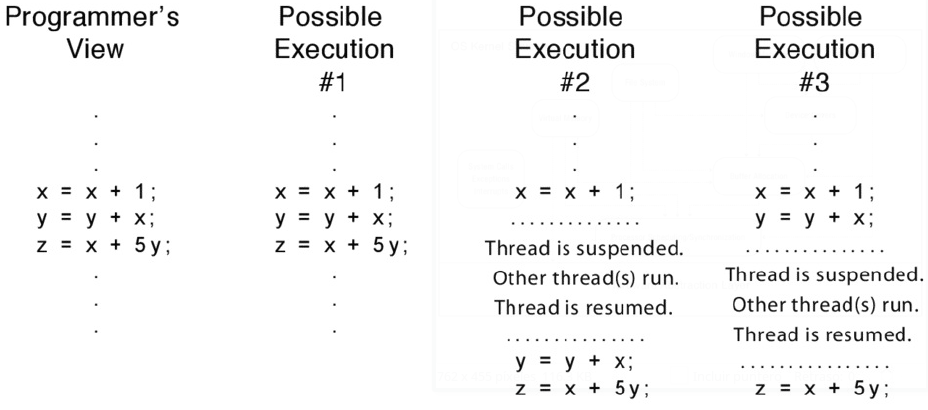
\includegraphics[scale=0.45]{img/fig15}}
\caption{Tres posibles formas en que un hilo puede ejecutar, todos los cuales son equivalentes al programador.}
\label{fig15}
\end{figure}

La \textit{fig.} \ref{fig15} ilustra la vista del programador de un programa sencillo y tres (de muchas) maneras posibles de cómo el programa puede ser ejecutado, dependiendo de lo que haga el planificador. Desde el punto de vista del hilo, o de la velocidad de ejecución, las alternativas son equivalentes. De hecho, el hilo típicamente no es consciente de cuál de estos (u otros) se produce en realidad durante la ejecución.

\begin{figure}[tbhp]
\centerline{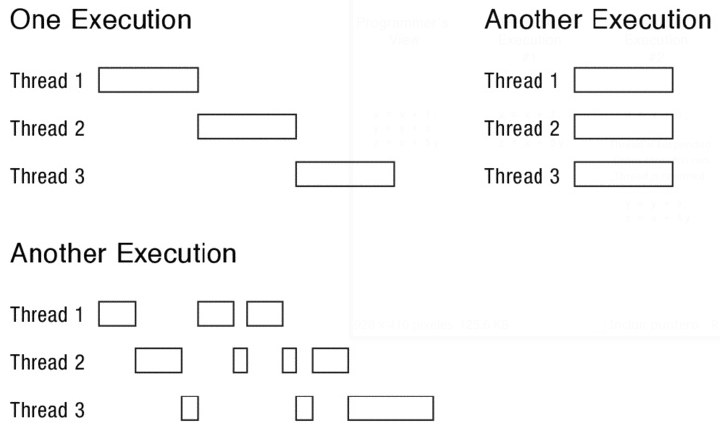
\includegraphics[scale=0.45]{img/fig16}}
\caption{Algunas de las muchas maneras posibles que podrían ser tres hilos intercalados en tiempo de ejecución.}
\label{fig16}
\end{figure}

¿Cómo se programan los hilos afecta a la intercalación de un hilo con otros hilos. La \textit{fug.} \ref{fig16} muestra algunas de las muchas posibles intercalaciones de un programa con tres hilos. El programador de hilos, por tanto, no debe hacer ninguna suposición sobre la velocidad relativa con la que ejecutan diferentes hilos.

\subsection{Por qué la Velocidad Variable?}
Puede parecer extraño requerir a los programadores suponer que el procesador virtual de un hilo corre a una velocidad impredecible y que cualquier intercalación con otros hilos es posible. Sin duda, el programador debe ser capaz de aprovechar el hecho de que algunos intercalados son más propensos que otros?

El modelo de programación con hilos adopta esta suposición como una forma de guiar a los programadores al razonar sobre la corrección. En lugar de asumir que un hilo corre a la misma velocidad que los otros (o más rápido o más lento) y tratando de escribir programas que coordinan los hilos sobre la base de su velocidad relativa de ejecución, los programas multihilo deben hacer suposiciones sobre el comportamiento del programador de subprocesos. A su vez, las decisiones de programación del kernel - cuando se asignan un hilo a un procesador, y al adelantarse por un subproceso diferente - se puede hacer sin tener que preocuparse en si podrían afectar a la corrección del programa.

Si los hilos son completamente independientes entre sí, sin compartir memoria u otros recursos, entonces la orden de ejecución no importa - cualquier momento producirá el mismo resultado que cualquier otro. La mayoría de los programas multihilo comparten estructuras de datos, sin embargo. En este caso, como el Capítulo 5 describe, el programador debe utilizar la sincronización explícita para garantizar la corrección del programa, independientemente de la posible intercalación de instrucciones de diferentes hilos.

Incluso si podíamos pasar por alto el tema de la programación - por ejemplo, si hay más procesadores que hilos de manera que cada hilo se le asigna su propio procesador físico - la realidad física es que la velocidad de ejecución relativa de los diferentes hilos puede verse afectado significativamente por factores fuera de su control. Un ejemplo extremo es que el programador puede estar depurando un hilo paso a paso, mientras que otros hilos corren a toda velocidad en otros procesadores. Si el programador ha de tener alguna esperanza de entender el comportamiento concurrente del programa, la corrección del programa no puede depender de que se esté cumpliendo con los hilos.

La variabilidad en la velocidad de ejecución se produce también durante el funcionamiento normal. El acceso a memoria puede estancar un procesador para cientos o miles de ciclos si se produce un fallo de caché. Otros factores incluyen la frecuencia con la que el programador tiene prioridad sobre el hilo, el número de procesadores físicos que están presentes en una máquina, el tamaño de las cachés, qué tan rápida es la memoria, cómo el firmware de ahorro de energía se ajusta la velocidad de reloj de los transformadores, los mensajes que llegan la red, o lo que se recibe de entrada del usuario. Las velocidades de ejecución de los diferentes hilos de un programa son difíciles de predecir, puede variar en un hardware diferente, e incluso puede variar de una ejecución a otra en el mismo hardware. Como resultado, hay que coordinar las acciones de hilo a través de la sincronización explícita en lugar de tratar de razonar acerca de su velocidad relativa.

\section{API de Hilo Simple}
Una buena manera de entender la API de hilos simples es que proporciona una manera de invocar una llamada a procedimiento asincrónico. Una llamada de procedimiento normal pasa a un conjunto de parámetros a la función, la función se ejecuta inmediatamente en la pila de la persona que llama, y cuando se termina la función, el control vuelve de nuevo a la persona que llama con el resultado. Una llamada a procedimiento asincrónico separa la llamada de la devolución: con \textit{thread\_ create}, la persona que llama inicia la función, pero a diferencia de una llamada a procedimiento normal, la persona que llama continúa la ejecución concurrente con la función llamada. Más tarde, el llamante puede esperar a la finalización de función (con \textit{thread\_ join}).

En el capítulo 3, vimos conceptos similares en la abstracción de proceso de UNIX. \textit{thread\_ create} es análogo al proceso fork y exec, mientras \textit{thread\_ join} es análogo al proceso de UNIX wait. UNIX fork crea un nuevo proceso que se ejecuta simultáneamente con el proceso llamando a fork; UNIX exec hace que ese proceso ejecute un programa específico. UNIX wait permite que el proceso de llamada suspenda la ejecución hasta la finalización del nuevo proceso.

\subsection{Paralelismo fork-join}
Muchas aplicaciones muilhilo pueden diseñarse utilizando sólo estas operaciones de hilo y ninguna sincronización adicional. Con paralelismo fork-join, un hilo puede crear hilos hijos para realizar el trabajo (\textit{fork} o \textit{thread\_ create}), y se puede esperar sus resultados (\textit{join}). Los datos pueden ser compartidos de forma segura entre los hilos, siempre que se proceda $(a)$ escrito por el padre antes de que el hilo hijo inicie o $(b)$ escrito por el hijo y leído por los padres después de la unión.

Si se siguen estas restricciones que comparten, cada hilo se ejecuta de forma independiente y de una manera determinista, no afectado por el comportamiento de cualquier otro hilo que se ejecuta simultáneamente. La multiplexación de hilos en procesadores no tiene otro efecto que el rendimiento.

\section{Estructura de Datos y Ciclo de Vida de un Hilo}
Como hemos visto, cada hilo representa una corriente secuencial de ejecución. El sistema operativo proporciona la ilusión de que cada hilo se ejecuta en su propio procesador virtual mediante la suspensión y reanudación de los hilos de forma transparente. Para que la ilusión funcione, el sistema operativo debe guardar con precisión y restaurar el estado de un hilo. Sin embargo, debido a que los hilos funcionan tanto en un proceso o en el núcleo, también hay estado compartido que no se guarda o se restaura cuando se cambia el procesador entre los hilos.

Por lo tanto, para entender cómo el sistema operativo implementa la abstracción hilo, hay que definir tanto el estado de cada subproceso y el estado que se comparte entre los hilos. Entonces podemos describir el ciclo de vida de un hilo - cómo el sistema operativo puede crear, iniciar, detener y eliminar hilos para proporcionar la abstracción.

\subsection{Bloque de Control de un Hilo y sus Estados - TCB}
El sistema operativo necesita una estructura de datos para representar el estado de un hilo; un hilo es como cualquier otro objeto en este sentido. Esta estructura de datos se llama el bloque de control de hilo (TCB). Para cada hilo que crea el sistema operativo, se crea una TCB.

El bloque de control del hilo lleva a cabo dos tipos de información para cada subproceso:
\begin{enumerate}
\item El estado de la computación que se realiza por el hilo.
\item Los metadatos sobre el hilo que se utiliza para gestionar el hilo.
\end{enumerate}

\textbf{Cálculo del Estado para cada subproceso.} Para crear múltiples hilos y ser capaz de iniciar y detener cada hilo, según sea necesario, el sistema operativo debe asignar espacio en el TCB para el estado actual de la ejecución de cada hilo: un puntero a la pila del subproceso y una copia de sus registros del procesador.

\begin{itemize}
\item \textbf{Pila.} La pila de un subproceso es la misma que la pila para un único subproceso de cálculo - que almacena información necesaria para que los procedimientos anidados el hilo se está ejecutando actualmente. Por ejemplo, si un subproceso llama foo(), foo() llama a bar(), y el bar() llama bas(), entonces la pila contendría un marco de pila para cada uno de estos tres procedimientos; cada marco de pila contiene las variables locales utilizados por el procedimiento, los parámetros del procedimiento se llama, y con la dirección de retorno a saltar a cuando finaliza el procedimiento.

Debido a que en un momento dado diferentes hilos pueden estar en diferentes estados en sus cálculos secuenciales - cada uno puede estar en un lugar diferente en un procedimiento distinto llamado con diferentes argumentos de un agrupamiento diferente de los procedimientos que encierra - cada hilo necesita su propia pila. Cuando se crea un nuevo hilo, el sistema operativo asigna una nueva pila y almacena un puntero a la pila en el TCB.

\item \textbf{Copia de los registros del procesador.} Los registros del procesador incluyen no sólo sus registros de propósito general para el almacenamiento de valores intermedios para los cálculos actuales, sino que también incluyen los registros de propósito especial, como el puntero de instrucción y puntero de pila.

Para poder suspender a un hilo, ejecutar otro hilo, y luego reanudar el hilo original, el sistema operativo necesita un lugar para almacenar los registros de un hilo cuando el hilo no se está ejecutando de forma activa. En algunos sistemas, los registros de propósito general para un hilo detenido se almacenan en la parte superior de la pila, y la TCB incluye solamente un puntero a la pila. En otros sistemas, el TCB contiene espacio para una copia de todos los registros del procesador.
\end{itemize}

\textbf{Los metadatos para cada subproceso.} El TCB también incluye metadatos para cada subproceso - información para la gestión de la rosca. Por ejemplo, cada hilo podría tener un ID de hilo, la prioridad de programación, y el estado (por ejemplo, si el hilo está esperando un evento o está listo para ser colocado en un procesador).

\subsection{Estados Compartidos}
La diferencia de estado para cada subproceso se asigna para cada hilo, algunos estados se comparten entre subprocesos que se ejecutan en el mismo proceso o en el núcleo del sistema operativo. En particular, el código del programa es compartido por todos los hilos en un proceso, aunque cada hilo puede estar ejecutando en un lugar diferente dentro de ese código. Además, estáticamente se asignan variables globales y dinámicamente se asignan las variables de la pila pueden almacenar información que es accesible a todos los hilos.

ADVERTENCIA: Aunque existe una división lógica importante entre el estado por hilo y estado compartido, el sistema operativo normalmente no hace cumplir esta división. Nada impide que un hilo con errores acceda al estado de un subproceso (conceptualmente privado) de otro hilo. Escribir mal un puntero a un hilo puede corromper la pila de otro. O un programador descuidado podría pasar un puntero a una variable local en la pila de un subproceso a otro hilo, dando el segundo hilo da un puntero a una ubicación de pila cuyo contenido puede cambiar a medida que las primeras llamadas de hilos y rendimientos de diversos procedimientos. O el primer hilo puede salir después de la entrega de un puntero a una variable en su pila; el montón reasignará que la memoria a un fin distinto. Debido a que estos errores pueden depender de las interleavings específicas de las ejecuciones hilos, que pueden ser extremadamente difíciles de localizar y corregir.

Para evitar comportamientos inesperados, es importante a la hora de escribir programas multihilo saber qué variables están diseñados para ser compartidas a través de hilos (variables globales, los objetos en la pila) y que están diseñados para ser (variables locales/automáticos) privadas.

\section{Ciclo de Vida de un Hilo}
Es útil tener en cuenta la progresión de estados de como un hilo pasa de ser creado, de ser programado y desprogramado de entrada y salida de un procesador, y luego a la salida. La \textit{fig.} \ref{fig17} muestra los estados de un hilo durante su vida útil.
\begin{figure}[tbhp]
\centerline{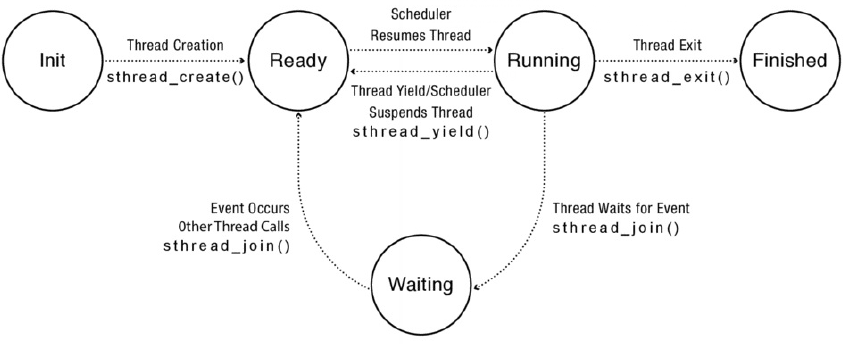
\includegraphics[scale=0.45]{img/fig17}}
\caption{Los estados de un hilo durante su vida útil.}
\label{fig17}
\end{figure}

\textbf{INIT (Inicio).} La creación del hilo pone un hilo en su estado INIT y asigna e inicializa las estructuras de datos por subproceso. Una vez hecho esto, el código de la creación del hilo pone al hilo en el estado READY mediante la adición del hilo a la READY LIST. Esta lista es el conjunto de hilos ejecutables que están esperando su turno para utilizar un procesador. En la práctica, la READY LIST no es en realidad una \textit{lista}; el sistema operativo utiliza típicamente una estructura de datos más sofisticado para realizar un seguimiento de hilos ejecutables, tales como una cola de prioridad. Sin embargo, después de la convención, vamos a seguir para referirse a ella como la lista preparada.

\textbf{READY (Listo).} Un hilo en el estado READY está disponible para ser ejecutado pero en la actualidad no se está ejecutando. Su TCB está en la READY LIST, y los valores de sus registros se almacenan en su TCB. En cualquier momento, el planificador puede causar que un hilo haga la transición de READY a RUNNING copiando sus valores de registro de su TCB a los registros de un procesador.

\textbf{RUNNING (En Ejecución).} Un hilo en estado de RUNNING se esta ejecutando en un procesador. En este momento, sus valores de registro se almacenan en el procesador en vez de en el TCB. Un hilo en estado RUNNING puede pasar al estado READY de dos maneras:
\begin{itemize}
\item El planificador puede adelantar un hilo en RUNNING y moverlo al estado READY por: $(1)$ el ahorro de los registros del hilo en su TCB y $(2)$ el cambio del procesador para ejecutar el siguiente hilo en la READY LIST.
\item Un hilo en estado RUNNING puede renunciar voluntariamente al procesador y pasar de EJECUCIÓN a LISTO por una llamada (por ejemplo, $thread\_ yield$ en la biblioteca de subprocesos).
\end{itemize}

Observe que un hilo puede pasar de READY a RUNNING y volver muchas veces. Dado que el sistema operativo guarda y restaura exactamente los registros de cada hilo, sólo la velocidad de ejecución del subproceso se ve afectada por estas transiciones.

\textbf{WAITING (En Espera).} Un hilo en el estado de WAITING está a la espera de algún acontecimiento. Mientras que el planificador puede mover un hilo en el estado LISTO al estado de EJECUCIÓN, un hilo en el estado de ESPERA no se puede ejecutar hasta que alguna acción por otro subproceso lo mueva de espera a LISTO.

Mientras que un hilo espera un evento, no se puede avanzar; Por lo tanto, no es útil para ejecutarlo. En lugar de seguir el hilo ejecutar o guardar la TCB en la lista de lista de la agenda, la TCB se almacena en la lista de espera de alguna variable de sincronización asociado con el evento. Cuando se produce el evento es necesario, el sistema operativo mueve el TCB de la lista de espera de la variable de sincronización a la lista de lista de la agenda, la transición desde el hilo a la espera de LISTO. Se describen las variables de sincronización en el capítulo 5.

\textbf{FINISHED (Terminado).} Un hilo en estado FINISHED nunca se ejecuta de nuevo. El sistema puede liberar parte o la totalidad de su estado para otros usos, aunque puede mantener algunos remanentes del hilo en la fase de producto terminado por un tiempo poniendo la TCB en una FINISHED LIST. Por ejemplo, la llamada $thread\_ exit$ permite pasar un hilo a su valor de salida a su padre a través del hilo $thread\_ join$. Finalmente, cuando el estado de un hilo ya no es necesario (por ejemplo, después de su valor de salida ha sido leído por unirse a la llamada), el sistema puede eliminar y recuperar el estado del hilo.

\section{Implementacion de Hilos en el Kernel}
Hasta ahora, hemos descrito las estructuras de datos básicos y el funcionamiento de un hilo. A continuación se describe cómo ponerlos en práctica. Los detalles de la aplicación varían en función del contexto:
\begin{itemize}
\item \textbf{Los hilos del núcleo.} La forma más simple de implementar hilos es en el interior del núcleo del sistema operativo, compartiendo uno o más procesadores físicos. Un hilo del núcleo ejecuta el código del núcleo y modifica las estructuras de datos del núcleo. Casi todos los sistemas operativos hoy en día soportan hilos en su núcleo.

\item \textbf{Los hilos del núcleo y los procesos de un único subproceso.} Un sistema operativo con los hilos del núcleo también puede ejecutar algunos procesos de usuario de un único subproceso. Estos procesos pueden invocar llamadas al sistema que se ejecutan al mismo tiempo que los hilos del núcleo en el interior del núcleo.

\item \textbf{Los procesos multihilos que utilizan los hilos del núcleo.} La mayoría de los sistemas operativos proporcionan un conjunto de rutinas y el sistema de bibliotecas para permitir a las aplicaciones utilizar múltiples hilos dentro de un solo proceso a nivel de usuario. Estos hilos ejecutan código de usuario y tienen estructuras de datos de acceso a nivel de usuario. También hacen llamadas al sistema en el núcleo del sistema operativo. Para ello, necesitan una pila de interrupciones del núcleo al igual que un proceso de un solo subproceso normal.

\item \textbf{Hilos a nivel de usuario.} Para evitar tener que hacer una llamada al sistema para cada operación, algunos sistemas soportan un modelo en el que las operaciones de hilos a nivel de usuario - crear, rendimiento, unión, la salida, y las rutinas de sincronización - su prestación en su totalidad en un nivel de usuario, sin necesidad de invocar el núcleo.
\end{itemize}

\subsection{Creación de un Hilo}
Hay tres pasos para crear un hilo:
\begin{enumerate}
\item \textbf{Asignarle un estado al hilo.} El primer paso en el constructor es asignar espacio el estado del hilo por subprocesos: la TCB y la pila. Como hemos mencionado, la TCB es la estructura de datos del sistema de hilos utiliza para manejar el hilo. La pila es un área de memoria para almacenar datos acerca de los procedimientos en curso; se guardará en memoria como cualquier otra estructura de datos.

\item \textbf{Inicializar el estado por subproceso.} Para inicializar el TCB, el constructor establece los registros de los nuevos hilos que se van a necesitar cuando el hilo se ponga en RUNNING. Cuando al hilo se le asigna un procesador, queremos que comienza a correr.

\item \textbf{Poner TCP en la READY LIST.} El último paso en la creación de un hilo es para establecer su estado de READY y poner el nuevo TCB en la READY LIST, lo que permite que el hilo se programe.
\end{enumerate}

\subsection{Eliminación de un Hilo}
Cuando un subproceso llama $thread\_ exit$, hay dos pasos para borrar el hilo:
\begin{itemize}
\item Retire el hilo de la READY LIST de modo que nunca se ejecutará de nuevo.
\item Liberar el estado para cada subproceso asignado para el hilo.
\end{itemize}

Aunque esto parece fácil, hay una sutileza importante: si un hilo se elimina en sí de la READY LIST y libera su propio estado por cada subproceso, entonces el programa puede salir con \textit{break}. Por ejemplo, si un hilo se remueve a sí mismo de la READY LIST, pero se produce una interrupción antes de que el hilo acabe desasignar su estado, hay una pérdida de memoria: que el hilo no se reanudará a desasignar su estado.

Peor aún, supongamos que un hilo libera su propio estado? El hilo puede terminar de ejecutar el código en $thread\_ exit$ si no tiene una pila? ¿Qué ocurre si se produce una interrupción justo después de la pila del hilo se ha desasigna? Si el código de cambio de contexto intenta guardar el estado del hilo actual, se va a escribir en la memoria de-asignado, posiblemente para almacenamiento que otro procesador ha asignado re por alguna otra estructura de datos. El resultado podría estar dañado memoria, donde el comportamiento específico depende de la secuencia precisa de eventos. Huelga decir que un error sería muy difícil de localizar.

Afortunadamente, hay una solución sencilla: un hilo no elimina su propio estado. En su lugar, algún otro flujo debe hacerlo. A la salida, las transiciones del hilo al estado FINISHED, mueve su TCB de la READY LIST a una lista de hilos terminados el planificador no debe funcionar nunca. El hilo puede cambiar de forma segura al siguiente hilo en la READY LIST. Una vez terminado el hilo ya no está en funcionamiento, es seguro que algún otro flujo libere el estado del hilo.

\subsection{Cambio de contexto para un hilo - Thread Context Switch}
Para dar soporte a múltiples hilos, también necesitamos un mecanismo para cambiar los flujos en ejecución y que están listas.

Un cambio de contexto suspende la ejecución de un hilo actualmente en ejecución y reanuda la ejecución de algún otro hilo. El SWITCH guarda los registros del hilo que se está ejecutando actualmente, la TCB y la pila del hilo, y luego se restauran los registros del nuevo hilo, su TCB y la pila, en el procesador.

Tenemos que responder a varias preguntas:
\begin{itemize}
\item ¿Qué desencadena un cambio de contexto?
\item ¿Cómo funciona un cambio de contexto voluntario (por ejemplo, una llamada a $thread\_ yield$)?
\item ¿Cómo un cambio de contexto involuntario difiere de uno voluntario?
\item ¿Qué hilo debe elegir el planificador para ejecutar a continuación?
\end{itemize}

\textbf{¿Qué desencadena un cambio de contexto de un hilo del núcleo?} Un cambio de contexto puede ser desencadenado por una llamada ya sea voluntario en la biblioteca de subprocesos, o una interrupción involuntaria o procesador de excepción.
\begin{itemize}
\item \textbf{Voluntario.} El hilo podría llamar a una función de biblioteca de procesos que desencadena un cambio de contexto. Por ejemplo, la mayoría de las bibliotecas de hilos proporcionan una llamada $thread\_ yield$ que permite que el hilo que se está ejecutando actualmente dé voluntariamente el procesador al siguiente hilo en la READY LIST. Del mismo modo, los $thread\_ join$ y $thread\_ exit$ suspenden la ejecución del hilo actual y empiezan a correr uno diferente.

\item \textbf{Involuntario.} Una interrupción o una excepción de procesador podría invocar un manejador de interrupciones. El hardware de interrupción guarda el estado del hilo en ejecución y ejecuta el código del controlador. El controlador puede decidir que algún otro hilo se debe ejecutar, y luego cambiar a él. Alternativamente, si el hilo actual debería continuar funcionando, el controlador restablece el estado del hilo interrumpido y reanuda la ejecución.

Por ejemplo, muchos sistemas de hilos están diseñados para asegurar que ningún hilo pueda monopolizar el procesador. Para lograr esto, se pusieron un temporizador de hardware para interrumpir el procesador periódicamente (por ejemplo, cada pocos milisegundos). El manejador de interrupción de temporizador guarda el estado del hilo en ejecución, escoge otro hilo para ejecutar, y se ejecuta ese hilo mediante la restauración de su estado anterior.

Otros eventos de hardware de E/S (por ejemplo, se pulsa una tecla del teclado, llega un paquete de red, o se completa una operación de disco) también invocan el manejador de interrupciones. En estos casos, así, los manipuladores de guardar el estado de la rosca actualmente en ejecución para que pueda ser restaurado más tarde. A continuación, ejecute el código del controlador, y cuando se realiza el controlador, o bien restaurar el estado del hilo actual, o cambiar a un nuevo hilo. Un nuevo hilo se ejecutará si el evento de E / S mueve un hilo en la lista preparada con una prioridad más alta que la rosca prefabricada en funcionamiento.
\end{itemize}

Independientemente, el sistema de hilo debe guardar el estado actual del procesador, de modo que cuando el hilo actual reanuda la ejecución, parece como si el evento nunca ocurrió excepto por algún tiempo después de haber transcurrido. Esto proporciona la abstracción de la ejecución del hilo en un procesador virtual con velocidad impredecible y variable.

Para simplificar las cosas, no queremos hacer un cambio de contexto involuntario mientras estamos en medio de uno voluntario. Al cambiar entre dos hilos, es necesario aplazar temporalmente interrupciones hasta que el cambio se haya completado, para evitar confusiones. Los procesadores contienen instrucciones privilegiadas para diferir y volver a habilitar las interrupciones.

\textbf{Cambio de Contexto Voluntario de un hilo del núcleo.} Debido a que un cambio voluntario es más sencillo de entender, empezamos allí. Un subproceso llama $thread\_ yield$ para renunciar voluntariamente al procesador y dar lugar a otro hilo. los registros del subproceso se copian en su TCB y la pila, y su reanudación se hará cuando el planificador lo elija.

El pseudo-código para $thread\_ yield$ convierte primero las interrupciones para evitar que el sistema de hilos intente hacer dos cambios de contexto al mismo tiempo. El pseudo-código a continuación, extrae el siguiente hilo para funcionar fuera de la lista preparada (si lo hay), y cambia a la misma.

El código $thread\_ switch$ puede parecer complicado, ya que se llama en el contexto del hilo anterior y termina en el contexto del nuevo hilo. Para que esto funcione, $thread\_ switch$ guarda el estado de los registros en la pila y guarda el puntero de pila sobre el TCB. A continuación, pasa a la pila del nuevo hilo, restaura el estado del nuevo hilo de pila del nuevo hilo, y devuelve a cualquier contador de programa se almacena en la nueva pila.

\textbf{Cambio Involuntario de Contexto en el núcleo.} El capítulo 2 explica lo que ocurre cuando una interrupción, una excepción, o una \textit{trap} interrumpe un proceso en ejecución a nivel de usuario: el hardware y el software funcionan juntos para salvar el estado del proceso interrumpido, ejecute controlador del núcleo, y restaurar el estado del proceso interrumpido.

El mecanismo es casi idéntico cuando una interrupción o una \textit{trap} desencadena un cambio de hilo entre hilos en el núcleo. Los tres pasos que se describen en el Capítulo 2 se modifican ligeramente:
\begin{enumerate}
\item \textbf{Guardar el estado.} Guarde los registros del hilo actualmente en ejecución por lo que el controlador puede ejecutar código sin interrumpir el hilo. El hardware ahorra algo de estado cuando se produce la interrupción o excepción, y el software guarda el resto del estado cuando el controlador ejecuta.

\item \textbf{Ejecutar el controlador del núcleo.} Ejecutar código del controlador del núcleo para manejar la interrupción o excepción. Desde ya estamos en modo kernel, no es necesario cambiar de usuario al modo kernel en este paso. Asimismo, no hay que cambiar el puntero de pila a la base de la pila de interrupción del núcleo. En cambio, podemos simplemente empujar variables de estado o de controlador guardados en la pila actual, a partir del puntero de pila actual.

\item \textbf{Restaurar el estado.} Restaurar los registros de la siguiente lista de rosca de modo que el hilo puede reanudar la ejecución en que se detuvo.
\end{enumerate}

En resumen, la comparación de un interruptor entre los hilos del núcleo de lo que ocurre en una transferencia en modo de usuario: $(1)$ no hay necesidad de cambiar los modos (y por lo tanto no hay necesidad de cambiar las pilas) y $(2)$ el controlador puede reanudar cualquier tema en el lista preparada en lugar de siempre reanudar el hilo o proceso que se acaba de suspensión.

\textbf{Detalles de implementacion.} En la mayoría de las arquitecturas de procesador, una forma sencilla (pero ineficaz) para intercambiar al siguiente hilo desde el interior de un manejador de interrupciones es llamar $thread\_ switch$ justo antes de regreso del guía. Como ya hemos visto, $thread\_ switch$ guarda el estado del hilo actual (es decir, el estado del controlador de interrupción) y cambia a la nueva hilo del núcleo. Cuando se reanuda el hilo original, volverá a partir $thread\_ switch$, y el pop de inmediato el contexto de interrupción de la pila, reanudando ejecución en el punto en que se interrumpió.

La mayoría de los sistemas, como Linux, hacen una pequeña optimización para mejorar el rendimiento de manejo de interrupciones. El estado de la rosca interrumpida ya está guardado en la pila, aunque sea en el formato especificado por la interrupción de hardware. En caso de modificar $thread\_ switch$ para guardar y restaurar los registros exactamente igual que la interrupción de hardware, a continuación, volver de una interrupción y reanudación de un hilo son la misma acción: ambos hacen estallar el marco de interrupción de la pila para reanudar el siguiente hilo para funcionar.

Por ejemplo, para que sea compatible con el hardware x86 de interrupción, la implementación del software de $thread\_ switch$ simularía el caso del hardware, ahorrando el puntero de instrucción de retorno y eflags registro antes de llamar PUSHAD para guardar los registros de propósito general. Después de cambiar a la nueva pila, sería llamar iret para reanudar el nuevo hilo, si el nuevo hilo fue suspendido por un evento de hardware o software de una llamada.

\section{Combinando hilos del Núcleo y un único subproceso de Usuario}
Un proceso es una ejecución secuencial de instrucciones, por lo que cada proceso a nivel de usuario incluye el subproceso del proceso. Sin embargo, un proceso es algo más que un hilo porque tiene su propio espacio de direcciones.

Debido a que un proceso contiene más que sólo un hilo, el bloque de control de proceso de cada proceso (PCB) necesita más información que un bloque de control de hilo (TCB) para un hilo del núcleo. Al igual que un TCB, una PCB para un proceso de un solo subproceso debe almacenar los registros del procesador cuando el subproceso del proceso no se está ejecutando. Además, el PCB tiene información sobre el espacio de direcciones del proceso; cuando se produce un cambio de contexto de un proceso a otro, el sistema operativo debe cambiar los appings de memoria virtual, así como el estado de registro.

Dado que la PCB y TCB representan cada uno un hilo, la READY LIST del núcleo puede contener una mezcla de PCB para los procesos y TCB para los hilos del núcleo. Cuando el planificador elige el siguiente hilo para ejecutar, se puede escoger uno u otro tipo. Un switch de hilo es casi idéntico si se cambia entre los hilos del núcleo o la conmutación entre el hilo de un proceso y un hilo del núcleo. En ambos casos, el switch guarda el estado del hilo que se está ejecutando actualmente y restaura el estado del siguiente hilo a ejecutar.

Como mencionamos en el capítulo 2, la mayoría de los sistemas operativos dedican una pila del núcleo de interrupción para cada proceso. De esta manera, cuando el proceso tiene que realizar una llamada al sistema, o en una interrupción o un procesador de excepción, las \textit{trap} de hardware en el kernel, guarda el estado del procesador a nivel de usuario, y se pone en marcha en un controlador específico en el núcleo. Una vez dentro del núcleo, el hilo de proceso se comporta exactamente igual que un hilo del núcleo - puede crear hilos (u otros procesos), el bloque (por ejemplo, en UNIX o en proceso de espera de E/S), y hasta la salida. Mientras que en el interior del núcleo, el proceso puede ser vaciado anteriormente por una interrupción del temporizador o E/S de eventos, y un proceso de mayor prioridad o hilo del núcleo puede ejecutar en su lugar. La pila de PCB y del núcleo para las tiendas de procesos adelantó tanto su estado actual del núcleo, así como el estado de nivel de usuario guardan cuando el proceso inicia la llamada al sistema.

Podemos reanudar un proceso en el núcleo usando $thread\_ switch$. Sin embargo, cuando reanudamos la ejecución del proceso a nivel de usuario después de la finalización de una llamada al sistema o interrupción, debemos restaurar su estado precisamente como lo fue con anterioridad: el valor correcto en sus registros, ejecutando en modo usuario, con el virtual correspondiente mapas de memoria, y así sucesivamente.

Un detalle importante es que muchas arquitecturas de procesadores tienen estado coprocesador adicional, por ejemplo, registros de coma flotante, para el código de nivel de usuario. Por lo general, el núcleo del sistema operativo no hace uso de operaciones de punto flotante. Por lo tanto, el núcleo no necesita guardar esos registros cuando se cambia entre los hilos del núcleo, pero no guardar y restaurar cuando se cambia entre los procesos.

\section{Implementación de Procesos Multihilo}
Hasta ahora, hemos descrito cómo implementar varios subprocesos que se ejecutan en el interior del núcleo del sistema operativo. Por supuesto, también queremos ser capaz de ejecutar programas de usuario también. Dado que muchos programas de usuario son de un solo subproceso, comenzamos con el caso simple de cómo integrar los hilos del núcleo y los procesos de un hilo. A continuación, nos dirigimos a diversas formas de implementar procesos multihilo, procesos con múltiples hilos. Todos los sistemas operativos modernos ampliamente utilizads apoyan tanto de los hilos del núcleo y los procesos multihilo. Ambos lenguajes de programación como Java, y las interfaces de la biblioteca estándar tales como POSIX y los hilos simples, utilizan este soporte del sistema operativo para proporcionar la abstracción hilo para el programador.

\subsection{Implementación de procesos multihilo que hacen uso de los hilos del kernel}
La forma más sencilla para soportar múltiples hilos por proceso es utilizar la aplicación hilo del núcleo que ya hemos descrito. Cuando un hilo del núcleo crea, elimina, suspende o reanuda, se puede utilizar una simple llamada de procedimiento. Cuando un hilo a nivel de usuario tiene acceso a la biblioteca de subprocesos para hacer las mismas cosas, se utiliza una llamada al sistema para pedir al kernel para hacer la operación en su nombre.

Un hilo en un proceso tiene:
\begin{itemize}
\item Una pila de nivel de usuario para ejecutar código de usuario.
\item Una pila del núcleo de interrupción para cuando este hilo hace que las llamadas al sistema, provoca una excepción procesador, o se interrumpe.
\item Una TCB kernel para guardar y restaurar el estado para cada subproceso.
\end{itemize}

Para crear un hilo, la biblioteca de usuario asigna una pila de nivel de usuario para el hilo y luego hace una llamada al sistema en el núcleo. El núcleo asigna un TCB y pila de interrupciones, y organiza el estado del hilo para iniciar la ejecución de la pila a nivel de usuario al comienzo del procedimiento solicitado. El núcleo necesita para almacenar un puntero a la TCB en el bloque de control del proceso; si el proceso sale, el núcleo debe terminar cualquier otros subprocesos que se ejecutan en el proceso.

Después de crear el hilo, el núcleo pone el nuevo hilo en la READY LIST, para ser ejecutado como cualquier otro hilo, y devuelve el identificador único para el programa de usuario a utilizar cuando se hace referencia a la creación de un hilo (por ejemplo, para unirse). \textit{Join}, \textit{Yield} y \textit{Exit} funcionan de la misma manera: se colocan en el kernel para realizar la función solicitada.

\subsection{La Aplicación de Hilos a Nivel de Usuario - Sin Soporte del Núcleo}
También es posible implementar los hilos como una biblioteca completamente a nivel de usuario, sin ningún apoyo del sistema operativo. Bibliotecas de hilos primero tomaron este enfoque a nivel de usuario puro por la sencilla razón de que algunos sistemas operativos soportaban procesos multihilo. Incluso una vez operativo el apoyo del sistema de las discusiones se generalizó, las discusiones a nivel de usuario puro se utilizan a veces para minimizar la dependencia de los distintos sistemas operativos y maximizar la portabilidad; por ejemplo, las primeras implementaciones de \textit{Java Virtual Machine de Sun (JVM)} implementan lo que se llama hilos verdes, una pura aplicación a nivel de hilos por el usuario.

La idea básica es simple. La biblioteca de subprocesos instancia todas sus estructuras de datos dentro del proceso: TCB, la lista de listas, la lista final, y las listas de espera todos son sólo estructuras de datos en el espacio de direcciones del proceso. A continuación, las llamadas a la biblioteca de subprocesos son llamadas a procedimiento sólo, similar a cómo se implementan las mismas funciones dentro de un núcleo de múltiples subprocesos.

Para el núcleo del sistema operativo, una aplicación multihilo con hilos verdes parece ser un proceso normal, de un solo subproceso. El proceso en su conjunto puede hacer llamadas al sistema, ya sea a intervalos de tiempo, etc. A diferencia de los hilos del núcleo, cuando un proceso que utiliza hilos verdes es mucho tiempo en rodajas, todo el proceso, incluyendo la totalidad de sus hilos, se suspende.

Una limitación de hilos verdes es que el núcleo del sistema operativo no es consciente del estado de la lista preparada nivel por el usuario. Si la aplicación realiza una llamada al sistema que bloquea la espera de E / S, el kernel no es capaz de ejecutar un hilo a nivel de usuario diferente. Del mismo modo, en un multiprocesador, el núcleo no puede ejecutar los diferentes subprocesos que se ejecutan en un único proceso en diferentes procesadores.

\textbf{Hilos a nivel de usuario de suscripción preferente.} Sin embargo, es posible en la mayoría de los sistemas operativos para aplicar la preferencia entre los hilos a nivel de usuario que está ejecutando dentro de un proceso. Como ya comentamos en el capítulo 2, la mayoría de los sistemas operativos proporcionan un mecanismo de llamada ascendente para entregar la notificación de eventos asíncronos a un proceso; en UNIX son los llamados gestores de señales. Los eventos típicos o señales incluyen el usuario pulsa "escape" o en UNIX "Control-C"; este informa a la aplicación para intentar salir limpiamente. Otro caso común es una interrupción de temporizador para señalar en tiempo real transcurrido. Para entregar un evento, el kernel suspende la ejecución del proceso y luego se reanuda funcionando a un controlador especificado por el código de usuario, típicamente en una pila upcall o señal separada.

Para poner en práctica preventiva multi-threading para algún proceso P:
\begin{enumerate}
\item La librería de hilos a nivel de usuario realiza una llamada al sistema para registrar un manejador de señales de temporizador y pila de señales con el kernel.
\item Cuando se produce una interrupción de temporizador de hardware, el hardware guarda el estado del registro P y corre el  controlador del núcleo.
\item En lugar de restaurar el registro de estado y reanudar P en que se interrumpió, P copias de controlador del kernel salvados registros en la pila de la señal P.
\item El kernel continúa con la ejecución de P en el manejador de la señal registrada en la pila de señales.
\item Las copias manejador de la señal el estado del procesador de la rosca a nivel de usuario adelantó desde la pila de señales de TCB de ese hilo.
\item El controlador de señal elige el siguiente hilo de correr, vuelve a habilitar el manejador de señal (el equivalente a volver a habilitar las interrupciones), y restaura el estado del nuevo hilo de su TCB en el procesador. ejecución con el estado (nueva) almacenado en la pila de señales.
\end{enumerate}

Este enfoque virtualiza interrupciones y excepciones del procesador, proporcionando un proceso de nivel de usuario con una imagen muy similar a la que el núcleo se pone cuando ocurren estos eventos.

\subsection{Implementación de Hilos a Nivel de Usuario - Con Soporte del Núcleo}
Hoy en día, la mayoría de los programas utilizan los hilos del núcleo soportado en lugar de hilos a nivel de usuario puros. los principales sistemas operativos soportan hilos utilizando abstracciones estándar, por lo que el tema de la portabilidad es un problema menor de lo que era antes.

Sin embargo, diversos sistemas toman más de un modelo híbrido, el intento de combinar el rendimiento de peso ligero y de control de aplicación a través de la programación que se encuentra en hilos a nivel de usuario, mientras se mantiene muchas de las ventajas de los hilos del núcleo.

\textbf{Hybrid Thread Join - Hilo hibrido de ingreso.} Las bibliotecas de hilos pueden evitar la transición al núcleo en ciertos casos. Por ejemplo, en lugar de hacer siempre una llamada del sistema para $thread\_ join$ esperar a que el subproceso de destino para terminar, $thread\_ exit$ puede almacenar su valor de salida en una estructura de datos en el espacio de direcciones del proceso. Entonces, si la llamada a $thread\_ join$ sucede después de que el hilo ha salido dirigida, puede devolver inmediatamente el valor sin tener que hacer una llamada al sistema. Sin embargo, si la llamada a $thread\_ join$ precede a la llamada a $thread\_ exit$, entonces se necesita una llamada al sistema para hacer la transición al estado de espera y dejar que alguna otra carrera hilo. Como optimización adicional, en un multiprocesador que a veces puede tener sentido para $thread\_ join$ a girar durante unos microsegundos antes de entrar en el núcleo, con la esperanza de que el otro hilo terminará en el ínterin.

\textbf{Hilos del Núcleo por Procesador.} Es posible adaptar el enfoque hilos verdes para trabajar en un multiprocesador. Para muchas aplicaciones científicas paralelas, el coste de la creación y la sincronización de hilos es de suma importancia, y por lo tanto un enfoque que requiere una llamada kernel para la mayoría de las operaciones de rosca sería prohibitivo. En su lugar, los hilos de los multicines de la biblioteca de nivel de usuario en la parte superior de los hilos del núcleo, exactamente de la misma manera que las roscas de los multicines del núcleo del núcleo en la parte superior de procesadores físicos.

Cuando se inicia la aplicación, la librería de hilos a nivel de usuario crea un hilo del núcleo de cada procesador en el equipo host. Mientras no hay otra actividad en el sistema, el kernel asignar cada uno de estos hilos un procesador. Cada hilo kernel inicia el programador de nivel de usuario en paralelo: tirar del hilo siguiente de la lista preparada a nivel de usuario, y ejecutarlo. Dado que las decisiones de programación hilo se producen a nivel de usuario, que puede ser flexible y específica de la aplicación; por ejemplo, en un algoritmo gráfico paralelo, el programador podría ajustar la prioridad de varios hilos a partir de los resultados del cálculo en otras partes de la gráfica.

Por supuesto, la mayoría de los inconvenientes de hilos verdes aún están presentes en estos sistemas:
\begin{itemize}
\item Cada vez que un hilo a nivel de usuario llama en el núcleo, sus secuencias de rosca núcleo de la máquina. Esto evita que la biblioteca de subprocesos de ejecución de un hilo a nivel de usuario diferente en ese procesador en el ínterin.
\item En cualquier momento en el kernel de tiempo-rebanadas de un hilo del núcleo, el hilo a nivel de usuario se ejecuta también está suspendido. La biblioteca no puede reanudar el hilo hasta que se reanude el hilo del núcleo.
\end{itemize}

\textbf{Las activaciones del planificador.} Para hacer frente a estos problemas, algunos sistemas operativos han añadido un apoyo explícito a las discusiones a nivel de usuario. Uno de estos modelos, más recientemente implementado en Windows, se llama activaciones del planificador. En este enfoque, se le notifica al planificador de hilos a nivel de usuario (o activa) para cada evento del núcleo que podrían afectar al sistema de rosca a nivel de usuario. Por ejemplo, si bloquea un hilo en una llamada al sistema, la activación informa al programador a nivel de usuario que debe elegir otro hilo se ejecute en ese procesador. activaciones del planificador son como upcalls o señales, excepto que no vuelven al núcleo; en cambio, realizan directamente hilo a nivel de usuario suspender y reanudar.

Diversas operaciones de desencadenar una llamada ascendente de activación planificador:
\begin{enumerate}
\item El aumento del número de procesadores virtuales. Cuando se inicia un programa, que recibe una activación para informar al programa que se ha asignado un procesador virtual: que la activación se ejecuta el hilo principal y cualquier otros hilos que pueden ser creados. Para asignar otro procesador virtual para el programa, el núcleo hace otra llamada ascendente de activación en el nuevo procesador; el planificador de nivel de usuario puede tirar de un hilo a la espera de la lista preparada y ejecutarlo.

\item La disminución de la cantidad de procesadores virtuales. Cuando el núcleo se adelanta a un procesador virtual (por ejemplo, para dar al procesador a un proceso diferente), el núcleo hace un llamada ascendente sobre uno de los otros procesadores asignados al programa paralelo. El sistema de hilos continuación, puede mover el hilo a nivel de usuario adelantó en la lista de listas, de modo que un procesador diferente puede ejecutarlo.

\item Transición a la espera. Cuando un hilo se bloquea a nivel de usuario en el kernel de espera de E / S, el kernel de manera similar hace un llamada ascendente a notificar al programador a nivel de usuario que tiene que tomar medidas, por ejemplo, para elegir otro hilo para funcionar a la espera de la E/S para completar.

\item Transición de espera a LISTO. Cuando la E/S completa, el núcleo hace una llamada ascendente a notificar al planificador que el hilo suspendido se puede reanudar.

\item La transición de RUNNING en marcha lenta. Cuando una activación a nivel de usuario encuentra una lista preparada vacío (es decir, no tiene más trabajo que hacer), se puede hacer una llamada al sistema en el kernel para devolver el procesador virtual para su uso por algún otro proceso.
\end{enumerate}

Como resultado, la mayoría de las funciones de gestión de hilo - $thread\_create$, $thread\_ yield$, $thread\_ exit$, y $thread\_ join$, así como las funciones de sincronización que se describen en el Capítulo 5 - se implementan como llamadas de procedimiento dentro del proceso. Sin embargo, el sistema de hilos a nivel de usuario siempre sabe exactamente cuántos procesadores virtuales que se le ha asignado y está en completo control de lo que se ejecuta en los procesadores.

\chapter{Sincronización de acceso a los objetos compartidos}
Los programas multihilo extienden el modelo tradicional, de un solo subproceso de programación de manera que cada hilo proporciona un único flujo secuencial de ejecución compuesto por instrucciones conocidas. Si un programa tiene hilos independientes que operan en subconjuntos completamente separados de la memoria, podemos razonar sobre cada hilo por separado. En este caso, el razonamiento acerca de los hilos independientes difiere poco del razonamiento acerca de una serie de programas independientes, de un único subproceso.

Sin embargo, la mayoría de los programas multihilo tienen tanto el estado para cada hilo (por ejemplo, registros de pila y un hilo) y el estado compartido (por ejemplo, variables compartidas en la pila). Los hilos de lectura y escritura cooperan con el estado compartido.

Compartir el estado es útil porque permite que los hilos se comuniquen, que coordinen el trabajo y compartan información. Por ejemplo, en el ejemplo de un GPS, una vez que un subproceso termina de descargar una imagen detallada de la red, comparte los datos de imagen con un hilo de renderizado que señala a la nueva imagen en la pantalla.

Por desgracia, cuando los hilos cooperan compartiendo sus estados, escribir programas multihilo correctos se vuelve mucho más difícil. La mayoría de los programadores están acostumbrados a pensar ''secuencialmente'' al razonar acerca de los programas. Por ejemplo, a menudo razonamos acerca de la serie de estados atravesados por un programa que ejecuta una secuencia de instrucciones. Sin embargo, este modelo secuencial de razonamiento no funciona en los programas de hilos cooperantes, por tres razones:

\begin{enumerate}
\item \textbf{La ejecución del programa depende de las posibles intercalaciones de acceso a hilos de estado compartido.} Por ejemplo, si dos hilos escriben una variable compartida, un hilo con el valor 1 y el otro con el valor 2, el valor final de la variable depende de cuál de los hilos acaba último.

Aunque este ejemplo es simple, el problema es grave porque los programas tienen que trabajar para cualquier posible intercalación. En particular, recuerdan que los programadores de hilos no deben hacer ninguna suposición sobre la velocidad relativa a la que operan sus hilos. Peor aún, como los programas crecen, hay una explosión combinatoria en el número de posibles intercalaciones.

\item \textbf{La ejecución del programa puede ser determinista.} Diferentes ejecuciones del mismo programa pueden producir resultados diferentes. Por ejemplo, el programador puede tomar diferentes decisiones de planificación, el procesador puede funcionar a una frecuencia diferente, u otro programa se ejecuta simultáneamente puede afectar a la caché de índice de aciertos. Incluso las técnicas de depuración comunes - como la ejecución de un programa con un depurador, volver a compilar con la opción -g en lugar de -O, o la adición de un printf - pueden cambiar el comportamiento de un programa.

Jim Gray, el ganador del premio ACM Turing 1998, acuñó el término \textit{Heisenbug} para los insectos que desaparecen o cambian el comportamiento cuando intenta examinarlos. La programación multihilo es una fuente común de heisenbug. Por el contrario, \textit{Bohrbugs} son deterministas y por lo general mucho más fácil de diagnosticar.

\item \textbf{Los compiladores y hardware del procesador pueden cambiar el orden de las instrucciones.} Los compiladores modernos e instrucciones de reabastecimiento de hardware mejoran el rendimiento. Esta reordenación es generalmente invisible para los programas de un solo subproceso; compiladores y procesadores de tener cuidado de asegurarse de que las dependencias dentro de una sola secuencia de instrucciones - es decir, dentro de un tema - se conservan. Sin embargo, el reordenamiento puede ser visible cuando varios subprocesos interactúan a través de acceso a variables compartidas.
\end{enumerate}

Teniendo en cuenta estos desafíos, el código multihilo puede introducir errores reproducibles sutiles, no deterministas, y no gubernamentales. En este capítulo se describe un enfoque estructurado para la sincronización del estado compartido en programas multihilo. En lugar de la dispersión de acceso a estos recursos compartidos en todo el programa e intentar razonamiento \textit{ad hoc} sobre lo que ocurre cuando se accede a los hilos se intercalan de diversas maneras, un mejor enfoque consiste en: $(1)$ la estructura del programa para facilitar el razonamiento acerca de la concurrencia, y $(2)$ utiliza un conjunto de primitivas de sincronización estándar para controlar el acceso a estos recursos compartidos. Este enfoque da un poco de libertad, pero si usted sigue constantemente las reglas que se describen en este capítulo, a continuación, el razonamiento sobre programas con estado compartido se convierte en mucho más simple.

La primera parte de este capítulo profundiza en los desafíos que enfrentan los programadores de subprocesos múltiples y el por qué es peligroso tratar de razonar acerca de todas las posibles intercalaciones de hilos en el caso general, no estructurada. El resto del capítulo describe la forma de estructurar los objetos compartidos en programas multihilo para que podamos razonar sobre ellos. En primer lugar, la estructura del Estado compartido de un programa multihilo como un conjunto de objetos compartidos que encapsulan el estado compartido, así como definir y limitar cómo se puede acceder al estado. En segundo lugar, para evitar el razonamiento \textit{ad hoc} sobre los posibles intercalamientos de acceso a las variables de estado dentro de un objeto compartido, se describe cómo los objetos compartidos pueden utilizar un pequeño conjunto de primitivas de sincronización - cerrojos y variables de condición - para coordinar el acceso a su estado por diferentes hilos. En tercer lugar, para simplificar el razonamiento sobre el código en objetos compartidos, se describe un conjunto de mejores prácticas para escribir el código que implementa cada objeto compartido. Por último, se profundiza en los detalles de cómo implementar primitivas de sincronización.

La programación multihilo tiene la reputación de ser difícil. Estamos de acuerdo en que se necesita atención, pero este capítulo proporciona un conjunto de reglas simples que cualquiera puede seguir para implementar los objetos que se pueden compartir con seguridad por varios subprocesos.

\section{Challenges - Desafíos}
Comenzamos este capítulo con el principal reto de la programación multihilo: la ejecución de un programa multihilo depende de los accesos intercalados del subproceso diferente a la memoria compartida, que pueden hacer que sea difícil para razonar acerca de depuración o de estos programas. En particular, la ejecución de hilos cooperantes puede verse afectada por las condiciones de carrera.

\subsection{Condiciones de Carrera}
Una condición de carrera se produce cuando el comportamiento de un programa depende de la intercalación de las operaciones de diferentes hilos. En efecto, los hilos corren una carrera entre sus operaciones y los resultados de la ejecución del programa depende de quién gane la carrera. Razonar sobre programas sencillos incluso con condiciones de carrera puede ser difícil. Para apreciar esto, ahora nos fijamos en tres programas multihilo muy simples.

\textbf{El programa de hilos cooperantes más simple del mundo.} Supongamos que ejecuta un programa con dos hilos que hacen lo siguiente: en el Hilo A se ejuta $x = 1$ y en el Hilo B se ejecuta $x = 2$. El resultado puede ser $x = 1$ o $x = 2$ dependiendo de qué hilo gane o pierda la carrera para setear el valor de $x$.

\textbf{El segundo programa de hilos cooperantes más pequeño del mundo.} Supongamos que en un principio $y = 12$, y se corre un programa con dos hilos que hacen lo siguiente: en el Hilo A se ejecuta $x = y + 1$ y en el Hilo B se ejecuta $y = y * 2$. El resultado es $x = 13$ si el subproceso A se ejecuta en primer lugar, o $x = 25$ si es B quien se ejecuta primero. Más precisamente, obtenemos $x = 13$ si el hilo A se lee antes de las actualizaciones del hilo B y, obtenemos $x = 25$ si las actualizaciones del hilo B se lee antes del hilo A.

\textbf{El tercer programa de hilos cooperantes mas pequeño del mundo.} Supongamos que en un principio $x = 0$ y se corre un programa con dos hilos que hacen lo siguiente: en el Hilo A se ejecuta $x = x + 1$ y en el Hilo B se ejecuta $x = x + 
$. Obviamente, un posible resultado es $x = 3$. Por ejemplo, el Hilo A se ejecuta hasta el final y luego el Hilo B se ejecuta hasta su finalización. Sin embargo, también podemos obtener $x = 2$ ó $x = 1$. En particular, cuando escribimos una sola declaración como $x = x + 1$, los compiladores de muchos procesadores producen múltiples instrucciones, tales como: $(1)$ la posición de memoria de carga de registros de $x$, $(2)$ añadir al menos $1$ de dicho registro, y $(3)$ almacenar el resultado de la posición de memoria $x$. Si desensamblamos el programa anterior en simples pseudo-ensamblaje de código, podemos ver algunas de las posibilidades.

\subsection{Operaciones Atómicas}
Cuando nos hemos desmontado el código en el último ejemplo, podríamos razonar acerca de las operaciones atómicas, operaciones indivisibles que no pueden ser intercaladas con o divididas por otras operaciones. En la mayoría de las arquitecturas modernas, una carga o almacenamiento (load o store) de una palabra de $32$ bits desde o a la memoria es una operación atómica. Por lo tanto, el análisis previo razonó sobre el intercalado de cargas y almacenamientos atómicos en la memoria.

Por el contrario, una carga o almacenamiento no es siempre una operación atómica. Dependiendo de la implementación de hardware, si dos hilos almacenan el valor de un registro de coma flotante de 64 bits a una dirección de memoria, el resultado final podría ser el primer valor, el segundo valor, o una mezcla de los dos.

\subsection{Too Much Milk - Demasiada Leche}
Aunque se podría, en principio, la razonar cuidadosamente acerca de las posibles intercalaciones de cargas y almacenamientos atómicos de diferentes hilos, hacerlo es complicado y propenso a errores. Más tarde, se presenta un mayor nivel de abstracción para la sincronización de hilos, pero primero se ilustran los problemas con el uso de las cargas y almacenamientos atómicos que utilizan un problema simple llamado, ''demasiada leche''. El ejemplo es deliberadamente sencilla; programas concurrentes del mundo real son a menudo mucho más compleja. Aun así, el ejemplo muestra la dificultad de razonar sobre el acceso a intercalada estado compartido. Los modelos de problemas de demasiada leche entre dos compañeros que comparten un refrigerador y que - como buenos compañeros - se aseguran de que el refrigerador esté siempre bien abastecido con leche.

Podemos modelar cada compañero de habitación como un hilo y el número de botellas de leche en la nevera con una variable en la memoria. Si las únicas operaciones atómicas en estado compartido son cargas y almacenamientos atómicos en la memoria, ¿hay una solución al problema de demasiada leche que garantiza tanto la seguridad (el programa nunca entra en mal estado) y la vida de la conexión (el programa entrará eventualmente en un buen estado)? Aquí, nos esforzamos por las siguientes propiedades:
\begin{itemize}
\item Safety (Seguridad): Nunca más de una persona compra la leche.
\item Liveness: Si se necesita la leche, alguien finalmente lo compra.
\end{itemize}

\textbf{Solución $1$.} La idea básica es que un compañero de habitación deje una nota en la nevera antes de ir a la tienda. La forma más sencilla de dejar esta nota - dado nuestro modelo de programación que hemos compartido memoria en el que podemos realizar cargas y amacenamiento atómicos - es fijar una bandera cuando va a comprar leche y para comprobar este indicador antes de ir a comprar leche.

Desafortunadamente, esta implementación puede violar la seguridad. Por ejemplo, el primer hilo podría ejecutar todo incluyendo la verificación del valor de la leche y luego el contexto ha cambiado. A continuación, el segundo hilo podría funcionar a través de todo este código y comprar leche. Por último, el primer hilo podría ser re-programado, ver se esa nota es cero, dejar la nota, comprar más leche, y eliminar la nota, dejando el sistema con $leche == 2$.

Esta ''solución'' empeora el problema. El código anterior por lo general funciona, pero puede fallar de vez en cuando el programador hace justo lo (mal o) lo correcto. Hemos creado una Heisenbug que hace que el programa falle ocasionalmente en formas que pueden ser muy difíciles de reproducir (por ejemplo, probablemente sólo cuando el alumno está mirando a ella o cuando el CEO está demostrando un nuevo producto en una feria comercial).

\textbf{Solución 2.} En la solución 1, el compañero de habitación comprueba la nota antes de ajustarla. Esto abre la posibilidad de que un compañero ya ha tomado la decisión de comprar la leche antes de notificar a la otro compañero de cuarto de esa decisión. Si utilizamos dos variables para las notas, un compañero puede crear una nota antes de comprobar la otra nota y tomar la decisión de comprar.

Si el primer hilo ejecuta la ruta de un código y el segundo hilo ejecuta el código, este protocolo es seguro; haciendo que cada hilo de escribir una nota (''yo podría comprar leche'') antes de decidirse a comprar leche, aseguramos la seguridad de la propiedad: a lo sumo un hilo compra leche.

Aunque esta intuición es sólida, lo que demuestra la propiedad de seguridad sin enumerar todas las posibles intercalaciones que  requieren cuidado.

\textbf{Safety Proof - Prueba de seguridad.} Supongamos por el bien de la contradicción que el algoritmo no es seguro - tanto A como B compran leche. Tenga en cuenta el estado de las dos variables (noteb, leche) cuando el hilo A está en la línea marcada A1, en el preciso momento cuando se produce la carga atómica de noteb de la memoria compartida para el registro de una. Hay tres casos a considerar:
\begin{itemize}
\item Caso 1: (noteB $= 1$, la leche = cualquier valor). Este estado contradice la suposición de que el hilo Una compra leche y llega a A3.
\item Caso 2: (noteb $= 0$, leche $> 0$). En este sencillo programa, la leche de la propiedad $> 0$ es una característica estable - una vez que se convierte en realidad, sigue siendo cierto para siempre. Por lo tanto, si la leche $> 0$ es cierto cuando A está en A1, la prueba de A en la línea A2 fallará, y A no va a comprar la leche, lo que contradice nuestra suposición.
\item Caso 3: (noteb $= 0$, leche $= 0$). Sabemos que el hilo B debe actualmente no se encuentre ejecutando cualquiera de las líneas marcadas B1-B5. También sabemos que, o bien NotaA $== 1$ o leche $> 0$ serán verdaderas de ahora en adelante (Notaa o leche es también una característica estable). Esto significa que B no puede comprar la leche en el futuro (ya sea en la prueba B1 o B2 debe fallar), lo que contradice nuestra suposición de que tanto A como B comprar leche.
\end{itemize}

Puesto que cada caso contradice la suposición, el algoritmo es seguro.

\textbf{Liveness - Vida de la conexión.} Por desgracia, la solución 2 no asegura la vida de la conexión. En particular, es posible que ambos hilos para establecer sus respectivas notas, para cada hilo para comprobar la nota del otro hilo, y por tanto de las discusiones para decidir no comprar leche. Esto nos lleva a la Solución 3.

\textbf{Solución 3.} La solución $2$ era seguro porque un hilo podría evitar la compra de leche si había alguna posibilidad de que el otro hilo podría comprar leche. Para la solución $3$, nos aseguramos de que al menos uno de los hilos determina si el otro hilo ha comprado la leche o no antes de decidir si comprar o no. En particular, hacemos lo siguiente:

Podemos demostrar que la solución $3$ es seguro usar un argumento similar al que se utilizó para la solución $2$. Para demostrar que la solución $3$ es en vivo, observar que ruta de código B no tiene bucles, por lo que finalmente el hilo B debe terminar de ejecutar el código en la lista. Con el tiempo, noteB $== 0$ se convierte en verdadera y sigue siendo cierto. Por lo tanto, el subproceso A debe finalmente llegar a la línea M y decidir si comprar la leche. Si encuentra $M == 1$, a continuación, la leche ha sido comprado. Si encuentra $M == 0$, entonces se va a comprar leche. De cualquier manera, la propiedad liveness - que, si es necesario, un poco de leche se compra - se cumple.

\subsection{Discusión}
Suponiendo que el compilador y el procesador ejecutan instrucciones en el orden del programa, la prueba anterior muestra que es posible idear una solución a demasiada leche que es a la vez Safety y Liveness usando nada más que las operaciones de carga y almacenamiento atómicas en la memoria compartida. Aunque la solución que presentamos sólo funciona para los dos compañeros, no es una generalización, llamado algoritmo de Peterson, que funciona con cualquier número fijo de $n$ hilos. Sin embargo, nuestra solución para demasiada leche (y así mismo algoritmo de Peterson) no es terriblemente satisfactorio:
\begin{itemize}
\item La solución es compleja y requiere un cuidadoso razonamiento para estar convencidos de que funciona.
\item La solución es ineficiente. En demasiada leche, mientras que el hilo A está a la espera, es una espera-ocupada que consumen recursos de la CPU. En solución generalizada de Peterson, todas las discusiones pueden n-ocupados esperar. Ls espera es especialmente problemática en los sistemas modernos con derecho preferente de subprocesos múltiples, como el hilo hilado puede estar reteniendo el procesador espera de un evento que no puede ocurrir hasta que se re-programado adelantó un poco de hilo para funcionar.
\item La solución puede fallar si el compilador o hardware reorganizan las instrucciones. Esta limitación puede abordarse mediante el uso de barreras de memoria (véase el recuadro). Adición de barreras de memoria aumentaría aún más la complejidad de la implementación del algoritmo; barreras no abordan las otras limitaciones que acabamos de mencionar.
\end{itemize}

\section{La estructura de los objetos compartidos}
\begin{figure}[tbhp]
\centerline{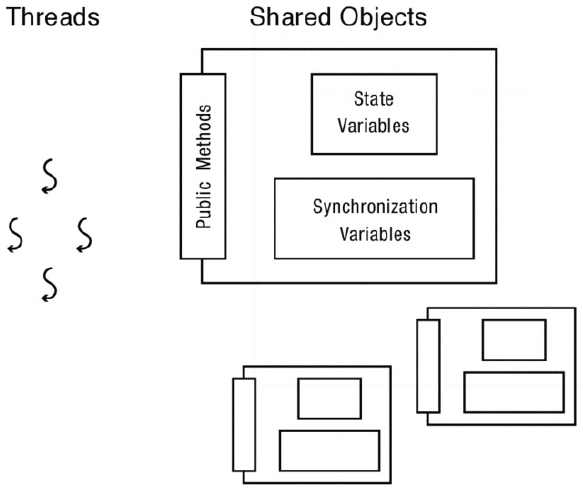
\includegraphics[scale=0.45]{img/fig0501}}
\caption{En un programa multi-hilo, hilos están separados y operan simultáneamente en objetos compartidos. Los objetos compartidos contienen ambas variables de estado y sincronización compartidos, que se utilizan para controlar el acceso concurrente a estado compartido.}
\label{fig0501}
\end{figure}

Décadas de trabajo han desarrollado un enfoque mucho más simple para escribir programas multihilo que el uso de cargas y almacenamientos atómicos. Este enfoque se extiende de la modularidad de la programación orientada a objetos para programas multihilo. Como ilustra la \textit{fig.} \ref{fig0501}, un programa multi-hilo se construye a partir de los objetos compartidos y un conjunto de hilos que operan en ellos.

Los objetos compartidos son objetos que se pueden acceder de manera segura por varios subprocesos. Todos estos recursos compartidos en un programa - incluyendo variables asignados en el montón (por ejemplo, objetos asignados con malloc o nuevo) y, variables globales estáticos - debe ser encapsulado en uno o más objetos compartidos.

Programar con objetos compartidos se extiende la programación tradicional orientado a objetos, en la cual los objetos ocultar sus detalles de implementación detrás de una interfaz limpia. De la misma manera, los objetos compartidos ocultar los detalles de la sincronización de las acciones de múltiples hilos detrás de una interfaz limpia. Los hilos que utilizan objetos compartidos sólo necesitan entender la interfaz; ellos no necesitan saber cómo el objeto compartido maneja internamente la sincronización.

Al igual que los objetos normales, los programadores pueden diseñar objetos compartidos para cualesquiera módulos, interfaces y semántica que necesita la aplicación. Cada clase de objeto compartido define un conjunto de métodos públicos en whichthreads operar. Para ensamblar el programa general de estos objetos compartidos, cada hilo se ejecuta un "bucle principal", escrita en términos de acciones sobre los métodos públicos de objetos compartidos.

Dado que los objetos compartidos encapsulan estado compartido del programa, el código de bucle principal que define medidas de alto nivel de un hilo no necesita preocuparse por los detalles de sincronización. Así, el modelo de programación se ve muy similar a la del código de un solo subproceso.

\subsection{La implementación de objetos compartidos}
Por supuesto, a nivel interno los objetos compartidos deben manejar los detalles de sincronización. Los objetos compartidos se aplican en capas.
\begin{itemize}
\item \textbf{Capa de objeto compartido.} Al igual que en la programación orientada a objetos estándar, los objetos compartidos definen la lógica específica de la aplicación y ocultan detalles internos de implementación. Externamente, parecen tener la misma interfaz que debe definir para un programa de un solo subproceso.

\item \textbf{Capa de sincronización de variable.} En lugar de la aplicación de los objetos compartidos directamente con
intercalado cuidadoso de las cargas y almacenamientos atómicos, los objetos compartidos incluyen variables de sincronización como variables miembro. las variables de sincronización, almacenados en la memoria al igual que cualquier otro objeto, pueden incluirse en cualquier estructura de datos.

Una variable de sincronización es una estructura de datos utilizada para coordinar el acceso simultáneo a estado compartido. Tanto la interfaz y la implementación de las variables de sincronización deben ser cuidadosamente diseñadas. En particular, podemos construir objetos compartidos utilizando dos tipos de variables de sincronización: Bloqueos (\textit{locks}) y Variables de Condición (\textit{condition variables}).

Las variables de sincronización coordinan el acceso a las variables de estado, que son sólo las variables miembros normales de un objeto que está familiarizado con la programación a partir de un único subproceso (por ejemplo, enteros, cadenas, arrays y punteros).

El uso de variables de sincronización simplifica la implementación de objetos compartidos. De hecho, no sólo los objetos compartidos se parecen externamente objetos de un único subproceso tradicionales, pero, mediante la aplicación, las variables de sincronización, sus implementaciones internas son bastante similares a los de los programas de un solo subproceso.

\item \textbf{La capa de instrucción Atómica.} A pesar de que las capas superiores se benefician de un modelo de programación más simple, no es tortugas hasta el final abajo. Internamente, las variables de sincronización deben gestionar los interleavings de acciones diferentes hilos.

En lugar de implementar las variables de sincronización, tales como cerrojos y variables de condición, utilizando cargas atómicas y tiendas como hemos tratado de hacer por el problema demasiada leche, las implementaciones modernas construyen las variables de sincronización utilizando instrucciones de lectura-modificación-escritura atómicas. Estas instrucciones específicos del procesador dejar un hilo tiene acceso de forma temporal y exclusiva atómica a una ubicación de memoria mientras se ejecuta la instrucción. Típicamente, la instrucción atómicamente lee una posición de memoria, hace alguna operación aritmética simple para el valor, y almacena el resultado. El hardware garantiza que las instrucciones de cualquier otro hilo con el acceso a misma posición de memoria se producen ya sea por completo antes de, o en su totalidad después de, la instrucción de lectura-modificación-escritura atómica.
\end{itemize}

\subsection{Alcance y Hoja de Ruta}
Los programas concurrentes se construyen en la parte superior de los objetos compartidos. El resto de este capítulo se centra en las capas medias de la figura - Cómo crear objetos compartidos utilizando objetos de sincronización y cómo construir objetos de sincronización de las órdenes de lectura-modificación-escritura atómicas. El capítulo 6 discute los problemas que surgen cuando se componen de varios objetos compartidos en un programa más amplio.

\section{Locks (Bloqueos): Exclusión Mutua}
Un bloqueo es una variable de sincronización que proporciona la exclusión mutua - cuando un hilo mantiene un bloqueo, ningún otro hilo puede mantenerlo (es decir, otros hilos están excluidos). Un programa tiene asociado cada cerrojo con algún subconjunto de estado compartido y requiere un hilo para mantener el bloqueo al acceder a ese estado. Entonces, sólo un hilo puede acceder al estado compartido a la vez.

La exclusión mutua simplifica en gran medida el razonamiento acerca de los programas ya que un subproceso puede realizar un conjunto arbitrario de operaciones, mientras que mantiene un bloqueo, y esas operaciones parecen ser atómicas a otros hilos. En particular, debido a que un bloqueo hace cumplir la exclusión mutua y los hilos deben sostener el bloqueo para acceder a estos recursos compartidos, ningún otro hilo puede observar un estado intermedio. Otros procesos únicamente pueden observar el estado de la izquierda después de la liberación del bloqueo.

\textbf{Bloqueo para agrupar varias operaciones.} Consideremos, por ejemplo, un objeto de cuenta de banco que incluye una lista de transacciones y un balance total. Para añadir una nueva transacción, adquirimos el bloqueo de la cuenta, añadir la nueva transacción a la lista, leer el antiguo equilibrio, modificarlo, escribir el nuevo equilibrio, y liberar el bloqueo. Para consultar el saldo y relación de las transacciones recientes, adquirimos bloqueo de la cuenta, leemos las transacciones recientes de la lista, lee el equilibrio, y liberar el bloqueo. El uso de cerrojos de esta manera garantiza que una actualización o una consulta completa antes de que comience la siguiente. Cada consulta siempre refleja el conjunto completo de transacciones recientes.

Otro ejemplo de agrupación es cuando la impresión de salida. Sin bloquear, si dos hilos llamados printf al mismo tiempo, los caracteres individuales de los dos mensajes podrían ser intercalados, garbling su significado. En cambio, en los sistemas operativos modernos multi-hilo, printf utiliza un cerrojo para asegurar que el grupo de caracteres en cada mensaje es impreso como una unidad.

Es mucho más fácil de razonar acerca de intercalación de grupos atómicos de operaciones en lugar de intercalar las operaciones individuales para dos razones. En primer lugar, hay un menor número (obviamente) interleavings a considerar. Razonar sobre interleavings sobre una base de grano más grueso reduce el número total de casos a considerar. En segundo lugar, y más importante, que podemos hacer cada grupo atómico de las operaciones corresponden a la estructura lógica del programa, lo que nos permite razonar sobre no invariantes interleavings específicos.

En particular, los objetos compartidos por lo general tienen un cerrojo que guarda todos estado de un objeto. Cada método público adquiere el bloqueo a la entrada y libera el bloqueo en la salida. Por lo tanto, el razonamiento sobre el código de una clase compartida es similar a razonar sobre el código de una clase tradicional: se asume un conjunto de invariantes cuando se llama a un método público y restablecer esas invariantes ante un público devuelve el método. Si definimos así nuestros invariantes, podemos razonar acerca de cada método de forma independiente.

\subsection{Cerrojos: API y Propiedades}
Un cerrojo permite la exclusión mutua, proporcionando dos métodos: Lock::adquieren() y Lock::Release(). Estos métodos se definen como sigue:
\begin{itemize}
\item Un bloqueo puede estar en uno de dos estados: ocupado o libre.
\item Un bloqueo se encuentra inicialmente en el estado libre.
\item Lock::adquirir espera hasta que el bloqueo es libre y luego atómicamente hace que el bloqueo OCUPADO. Comprobación del estado para ver si está libre y el establecimiento del estado de OCUPADO están juntos una operación atómica. Incluso si varios subprocesos intentan adquirir el bloqueo, a lo sumo un hilo tendrá éxito. Un hilo observa que el bloqueo es gratis y lo establece en OCUPADO; los otros hilos acaba de ver que el1 cerrojo está ocupado y esperan.
\item Lock::Bloquear la liberación hace que el bloqueo GRATIS. Si hay operaciones pendientes adquirir, este cambio de estado hace que uno de ellos para proceder.
\end{itemize}

Se describe cómo implementar los cerrojos con estas características en la sección 5.7. El uso de bloqueos hace que la solución del problema de la leche demasiado trivial. Ambos hilos corren el siguiente código:


\subsection{Semáforos}
Los \textbf{semáforos} fueron introducidos por Dijkstra en 1965 para proveer de sincronización dentro del sistema operativo. Entre los avances introducidos en el diseño de sistemas operativos se puede mencionar las formas estructuradas de utilización de la concurrencia.

Lo semáforos se definen como sigue:
\begin{itemize}
\item Un semáforo tiene un valor entero no negativo ($\geq 0$).
\item Cuando un semáforo es creado, su valor puede ser inicializado en cualquier valor entero no negativo.
\item {\mf Semaphore::P()} espera hasta que el valor sea positivo. Luego, decrementa su valor de manera atómica en 1 y retorna.
\item {\mf Semaphore::V()} incrementa de manera atómica el valor en 1. Si algún hilo se encuentra esperando en {\mf P}, entonces uno es habilitado, de forma que la llamada a {\mf P} puede decrementar exitosamente el valor y retornar.
\item No se permiten otras operaciones en un semáforo. En particular, ningún hilo puede leer directamente el valor del semáforo.
\end{itemize}

Las acciones de comprobar el valor y modificarlo se realizan en conjunto como una sola acción atómica indivisible. Se garantiza que, una vez que empieza una operación de semáforo, ningún otro proceso podrá acceder al semáforo sino hasta que la operación se haya completado o bloqueado. Esta atomicidad es absolutamente esencial para resolver problemas de sincronización y evitar condiciones de carrera.

La operación {\mf V} incrementa el valor del semáforo direccionado. Si uno o más procesos estaban inactivos en ese semáforo, sin poder completar una operación {\mf P} anterior, el sistema selecciona uno de ellos (al azar) y permite que complete su operación {\mf P} . Así, después de una
operación {\mf V} en un semáforo que contenga procesos inactivos, el semáforo seguirá en 0 pero habrá un proceso menos inactivo en él. La operación de incrementar el semáforo y despertar a un proceso también es indivisible. Ningún proceso se bloquea al realizar una operación {\mf V}.

Lo normal es implementar {\mf V} y {\mf P} como llamadas al sistema, en donde el sistema operativo deshabilita brevemente todas las interrupciones, mientras evalúa el semáforo, lo actualiza y pone el proceso a dormir, si es necesario. Como todas estas acciones requieren sólo unas cuantas instrucciones, no hay peligro al deshabilitar las interrupciones. Si se utilizan varias CPUs, cada semáforo debe estar protegido por una variable lock para asegurar que sólo una CPU a la vez pueda examinar el semáforo.

Los sistemas operativos diferencian a menudo entre semáforos contadores y semáforos binarios. El valor de un \textbf{semáforo contador} puede variar en un dominio no restringido, mientras que el valor del \textbf{semáforo binario} sólo puede ser 0 ó 1. En algunos sistemas, los semáforos binarios se conocen como \textbf{cerrojos mútex}, ya que son cerrojos que proporcionan exclusión mutua. Cuando el recurso está disponible, un proceso accede y decrementa el valor del semáforo con la operación P. El valor queda entonces en 0, lo que hace que si otro proceso intenta decrementarlo tenga que esperar. Cuando el proceso que decrementó el semáforo realiza una operación V, algún proceso que estaba esperando comienza a utilizar el recurso.

Los semáforos contadores se pueden utilizar para controlar el acceso a un determinado recurso formado por un número finito de instancias. El semáforo se inicializa con el número de recursos disponibles. Cada proceso que desee usar un recurso ejecuta una operación {\mf P()} en el semáforo (decrementando la cuenta). Cuando un proceso libera un recurso, ejecuta una operación {\mf V()} (incrementando la cuenta). Cuando la cuenta del semáforo llega a 0, todos los recursos estarán en uso. Después, los procesos que deseen usar un recurso se bloquearán hasta que la cuenta sea mayor a que 0.

También podemos usar los semáforos para resolver diversos problemas de sincronización. Por ejemplo, considere dos procesos que se estén ejecutando de forma concurrente: {\mf P1} con una instrucción {\mf S1} y {\mf P2} con una instrucción {\mf S2}. Suponga que necesitamos que {\mf S2} se ejecute sólo después que {\mf S1} se haya completado. Podemos implementar este esquema dejando que {\mf P1} y {\mf P2} compartan un semáforo común {\mf synch}, inicializado con el valor 0, e insertando las instrucciones:

\lstset{
	language=C++,
    basicstyle=\ttfamily,
	keywordstyle=\color{blue}\ttfamily,
    stringstyle=\color{red}\ttfamily,
	commentstyle=\color{green}\ttfamily,
    morecomment=[l][\color{magenta}]{\#}
}

\begin{lstlisting}
S1;
V(synch);
\end{lstlisting}

en el proceso {\mf P1}, y las instrucciones

\begin{lstlisting}
S2;
P(synch);
\end{lstlisting}

en el proceso {\mf P2}. Dado que {\mf synch} se inicializa con el valor 0, {\mf P2} ejecutará {\mf S2} sólo después de que {\mf P1} haya invocado 
V(synch), instrucción que sigue a la ejecución de {\mf S1}.

\setcounter{chapter}{6}
\chapter{Scheduling - Planificación}
Cuando hay varias cosas por hacer, cómo podemos elegir qué hacer primero? En los últimos capítulos, hemos descrito cómo crear subprocesos, intercalar entre ellos y sincronizar su acceso a los datos compartidos. En momento dado, algunos subprocesos se están ejecutando en el procesador. Otros están esperando su turno para ocupar el procesador. Mientras otros se bloquean esperando que se complete alguna E/S, se señale una variable de condición o se libere un bloqueo. Cuando hay más subprocesos que procesadores, la \textbf{política de programación del procesador} determina qué subprocesos ejecutar primero.

Podríamos pensar que la respuesta a esta pregunta es fácil: simplemente haga el trabajo en el orden en que llega. Después de todo, eso parece ser la única cosa justa a hacer. Hay una razón por la cual, como veremos más adelante en este capítulo, hacer las cosas por orden de llegada es a veces lo peor que puedes hacer en términos de mejorar el tiempo de respuesta percibido por el usuario.

Se podría pensar que la respuesta a esta pregunta no es importante. Con la mejora de millones de veces en el rendimiento del procesador en los últimos treinta años, podría parecer que somos un millón de veces menos propensos a tener nada esperando su turno de ocupar un procesador. Pero en verdad esto no es así, los sistemas operativos del servidor en particular son a menudo sobrecargados. Las aplicaciones paralelas pueden crear más cantidad de trabajo que procesadores existentes, y si no se toma en cuenta en el diseño de la política de planificación, el rendimiento puede degradarse gravemente. Hay relaciones sutiles entre la política de planificación y la administración de energía en los dispositivos con baterías, como los smartphones y las laptops. Además, los problemas de planificación se aplican a cualquier recurso escaso, ya sea que la fuente de contención sea el procesador, la memoria, el disco o la red.

La política de programación no es una panacea. Sin suficiente capacidad, el rendimiento puede ser pobre, independientemente del hilo que ejecutamos primero.

Afortunadamente, es probable que tengas un poco de intuición en cuanto al impacto de diferentes políticas y capacidad de planificación en temas como tiempo de respuesta, imparcialidad y rendimiento. Cualquier persona que espera en línea probablemente se pregunta cómo podríamos conseguir la línea para ir más rápidamente. Eso es cierto si estamos esperando en la fila en el supermercado, un banco, o en un restaurante popular. Sorprendentemente, en cada uno de estos entornos, hay un enfoque diferente de cómo se ocupan de la espera. Intentaremos responder por qué.

No hay una respuesta correcta; Más bien, cualquier política de planificación plantea un conjunto complejo de compensaciones entre varias propiedades deseables. El objetivo de este capítulo no es enumerar todas las posibilidades interesantes, explorar el espacio de diseño completo, ni siquiera identificar políticas útiles específicas. En cambio, describimos algunos de las compensaciones e intentamos ilustrar cómo un diseñador puede abordar el problema de seleccionar una política de planificación.

\textbf{Terminología de Rendimiento:}

\begin{itemize}
\item \textbf{Task - Tarea}. Una solicitud de usuario. Una tarea también se llama a menudo un trabajo. Una tarea puede ser de cualquier tamaño, desde simplemente volver a dibujar la pantalla para mostrar el movimiento del cursor del ratón hasta calcular la forma de una proteína recién descubierta. Cuando hablamos de planificación, usamos el término tarea, en lugar de hilo o proceso, porque un solo hilo o proceso puede ser responsable de múltiples solicitudes o tareas de usuario. Por ejemplo, en un procesador de palabras, cada carácter escrito es una solicitud de usuario individual para agregar ese carácter al archivo y mostrar el resultado en la pantalla.
\item \textbf{Response Time- Tiempo de respuesta (o Retardo)}. El tiempo percibido por el usuario para hacer alguna tarea.
\item \textbf{Predictability - Previsibilidad}. Baja variación en los tiempos de respuesta para solicitudes repetidas.
\item \textbf{Throughput - Rendimiento}. La velocidad a la que se completan las tareas.
\item \textbf{Scheduling Overhead - Sobrecarga de Planificación}. El tiempo para cambiar de una tarea a otra.
\item \textbf{Fairness - Equidad}. Igualdad en el número y puntualidad de los recursos asignados a cada tarea.
\item \textbf{Starvation - Inanición}. La falta de progreso de una tarea, debido a que los recursos fueron asignados a una tarea de mayor prioridad.
\end{itemize}

\section{Planificación de un solo Procesador}
Comenzamos con tres políticas sencillas: \textit{First-In-First-Out, Shortest-Job-First, and Round-Robin} (primero en entrar-primero en salir, primero el mas corto y en ronda), como una forma de ilustrar los conceptos de programación. Cada enfoque tiene sus propias fortalezas y debilidades, y la mayoría de los sistemas de asignación de recursos (ya sea para procesadores, memoria, red o disco) combinan aspectos de los tres. Al final de la discusión, mostraremos cómo los diferentes enfoques se pueden sintetizar en un planificador de procesador más práctico y completo.

Antes de proceder, necesitamos definir algunos términos. Una carga de trabajo (\textit{workload}) es un conjunto de tareas que debe realizar un sistema, junto con el momento en que llega cada tarea y cuánto tarda cada tarea en completarse (cuándo llega y cuánto tarda cada tarea). En otras palabras, la carga de trabajo define la entrada a un algoritmo de planificación. Dada una carga de trabajo, un planificador de procesador decide cuándo se asigna cada tarea al procesador.

Estamos interesados en programar algoritmos que funcionen bien en una amplia variedad de entornos, ya que las cargas de trabajo variarán bastante de sistema a sistema y de usuario a usuario. Algunas tareas se calculan y sólo utilizan el procesador. Otros, como un compilador o un navegador web, mezclan E/S y computo. Otros, como una descarga de BitTorrent, están vinculados a E/S, pasando la mayor parte de su tiempo esperando por E/S y sólo por períodos cortos de computo. En la discusión, comenzamos con cargas de trabajo muy complejas y luego generalizamos para incluir mezclas de diferentes tipos de tareas a medida que avanzamos.

Algunas de las políticas que describimos son la mejor política posible sobre una métrica y una carga de trabajo concretas, y algunas son la peor política posible. Al discutir la optimalidad y la pessimalidad, sólo estamos comparando con las políticas que son de conservación del trabajo. Un programador es conservador de trabajo si nunca deja el procesador inactivo si hay trabajo que hacer. Obviamente, una política trivialmente pobre tiene el procesador sentado inactivo durante largos períodos cuando hay tareas en la \textit{Ready List}.

Nuestra discusión asume también que el planificador tiene la capacidad de \textit{preempt} (pausar) al procesador y de darlo a alguna otra tarea. La Preemption puede ocurrir debido a una interrupción del temporizador, o porque alguna tarea llega a la \textit{Ready List} con una prioridad más alta que la tarea actual, al menos de acuerdo con alguna política de programación.

\subsection{Primero en entrar, primero en salir (FIFO)}
Tal vez el algoritmo de programación más simple \textbf{FIFO}: hacer cada tarea en el orden en que llega. FIFO a veces también se llama primero llegado primero servido, o \textbf{FCFS}. Cuando empezamos a trabajar en una tarea, seguimos funcionando hasta que termina. FIFO minimiza la sobrecarga, cambiando entre las tareas sólo cuando cada una esta completa. Debido a que minimiza la sobrecarga, si tenemos un número fijo de tareas, y esas tareas sólo necesitan el procesador, FIFO tendrá el mejor rendimiento: se completará la mayoría de las tareas más rápidamente. Y como mencionamos, FIFO parece ser la definición de la justicia - cada tarea espera pacientemente su turno.

Desafortunadamente, FIFO tiene una debilidad. Si una tarea corta con muy poco trabajo llega despues de comenzada una tarea que toma un tiempo muy largo, entonces el sistema parecerá muy ineficiente. La Figura \ref{fig0701} ilustra una carga de trabajo particularmente mala para FIFO. Si la primera tarea de la cola toma un segundo, y los cuatro siguientes llegan un instante después, pero cada uno sólo necesita un milisegundo del procesador, entonces todos tendrán que esperar hasta que termine el primero. El tiempo de respuesta promedio será más de un segundo, pero el tiempo de respuesta promedio óptimo es mucho menor que eso. De hecho, si ignoramos la conmutación de gastos generales, hay algunas cargas de trabajo donde FIFO es literalmente la peor política posible para el tiempo de respuesta promedio.

\textbf{FIFO y Memcached}

Aunque usted puede pensar que FIFO es demasiado simple para ser útil, hay algunos casos importantes donde es exactamente la elección correcta para la carga de trabajo. Un ejemplo de ello es memcached. Muchos servicios web, como Facebook, almacenan sus datos de usuario en una base de datos. La base de datos proporciona búsquedas flexibles y coherentes, como por ejemplo, qué amigos deben ser notificados de una actualización concreta en el murok de un usuario.

Con el fin de mejorar el rendimiento, Facebook y otros sistemas ponen un caché llamado memcached frente a la base de datos, de modo que si un usuario envía dos elementos a su muro, el sistema sólo tiene que buscar la lista de amigos una vez. El sistema comprueba primero si la información se almacena en caché y, si es así, utiliza esa copia.

Debido a que casi todas las solicitudes son para pequeñas cantidades de datos, memcached responde a peticiones en orden FIFO. Esto minimiza la sobrecarga, ya que no hay necesidad de intervalo de tiempo entre las solicitudes. Para esta carga de trabajo donde las tareas son aproximadamente iguales en tamaño, FIFO es simple, minimiza el tiempo de respuesta promedio e incluso maximiza el rendimiento. \textit{Win-Win!}

\subsection{El trabajo más corto primero (SJF)}
Si FIFO puede ser una mala elección para el tiempo de respuesta promedio, ¿Existe una política óptima para minimizar el tiempo de respuesta promedio? La respuesta es sí: planificar el trabajo más corto primero (SJF).

Supongamos que podríamos saber cuánto tiempo necesita cada tarea en el procesador. (En general, no lo sabremos, por lo que no se trata de una política práctica, sino que la utilizamos como un experimento de pensamiento, más adelante veremos cómo aproximar a SJF en la práctica). Si siempre planificamos la tarea que tiene el trabajo mas corto por hacer, se minimiza el tiempo de respuesta promedio. (Por esta razón, algunos llaman a SJF shortest-remaining-time-first o \textbf{SRTF}.)

Para ver que el SJF es óptimo, considere una hipotética política alternativa que no sea SJF, pero que creemos que podría ser óptima. Dado que la alternativa no es SJF, en algún momento elegirá ejecutar una tarea que sea más larga que otra en la cola. Si ahora cambiamos el orden de tareas, manteniendo todo igual, pero haciendo la tarea más corta primero, reduciremos el tiempo de respuesta promedio. Por lo tanto, cualquier alternativa a SJF no puede ser óptima.

La Figura \ref{fig0701} ilustra SJF en el mismo ejemplo que usamos para FIFO. Si una tarea larga es la primera en llegar, se programará (si estamos conservando el trabajo). Cuando una tarea corta llega un poco más tarde, el programador prevé la tarea actual, e inicia la más corta. Las restantes tareas cortas serán procesadas en orden de llegada, seguido de terminar la tarea larga.

Lo que cuenta como "más corto" es el tiempo restante en la tarea, no su longitud original. Si estamos a un nanosegundo de terminar una tarea de una hora de duración, minimizaremos el tiempo de respuesta promedio manteniéndonos con esa tarea, en lugar de evitarla por una tarea de un minuto que acaba de llegar a la \textit{Ready List}. Por supuesto, si ambos llegan casi al mismo tiempo, hacer la tarea de un minuto de duración primero mejorará drásticamente el tiempo de respuesta promedio.

¿Tiene SJF otros inconvenientes (aparte de ser imposible de implementar porque requiere conocimiento del futuro)? Resulta que SJF es pesimal para la variación en el tiempo de respuesta. Haciendo las tareas más cortas lo más rápido posible, SJF hace necesariamente tareas más largas lo más lentamente posible (entre las políticas que son conservadoras de trabajo). En otras palabras, existe una compensación fundamental entre reducir el tiempo de respuesta promedio y reducir la varianza en el tiempo de respuesta promedio.

Peor aún, SJF puede sufrir de hambre y frecuentes cambios de contexto. Si llegan suficientes tareas cortas, las tareas largas pueden no completarse. Siempre que una tarea nueva en la \textit{Ready List} sea más corta que el tiempo restante restante en la tarea actual, el planificador cambiará a la nueva tarea. Si esto sigue sucediendo indefinidamente, una larga tarea puede no terminar nunca.

\begin{figure}[tbhp]
\centerline{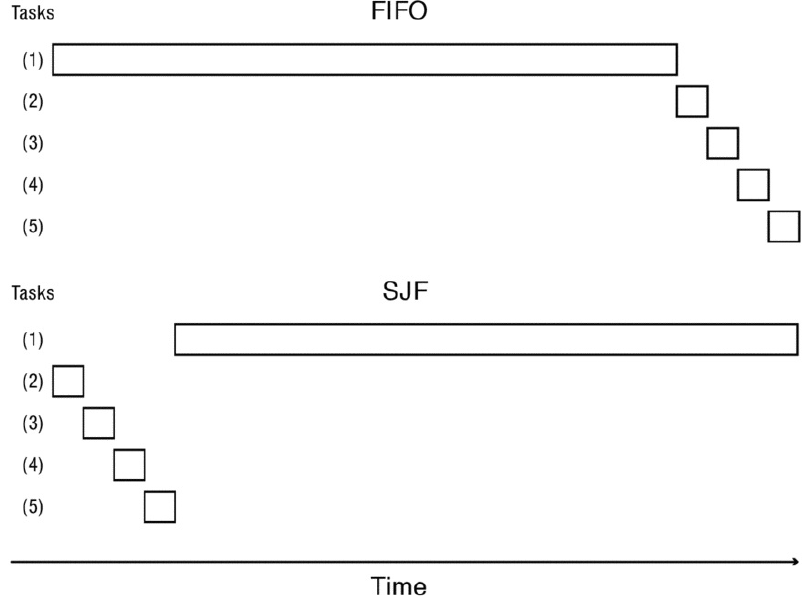
\includegraphics[scale=0.70]{img/fig0701}}
\caption{Los tiempos de finalización con FIFO (arriba) y SJF (abajo) de la planificación cuando varias tareas cortas ($2-5$) llegan inmediatamente después de una tarea larga ($1$).}
\label{fig0701}
\end{figure}

\subsection{Round Robin}
Una política que aborda el hambre es programar las tareas de una manera Round Robin. Con Round Robin, las tareas se turnan ejecutándose en el procesador durante un período limitado de tiempo. El planificador asigna el procesador a la primera tarea en la \textit{Ready List}, estableciendo una interrupción del temporizador para un cierto retardo, llamado el tiempo cuántico. Al final del quantum, si la tarea no se ha completado, la tarea se evita y el procesador se da a la siguiente tarea en la \textit{Ready List}. La tarea anticipada se vuelve a poner en la \textit{Ready List} donde puede esperar su siguiente turno. Con Round Robin, no hay posibilidad de que una tarea se muera de hambre. Finalmente llegará al frente de la cola y obtendrá su tiempo cuántico.


\begin{figure}[tbhp]
\centerline{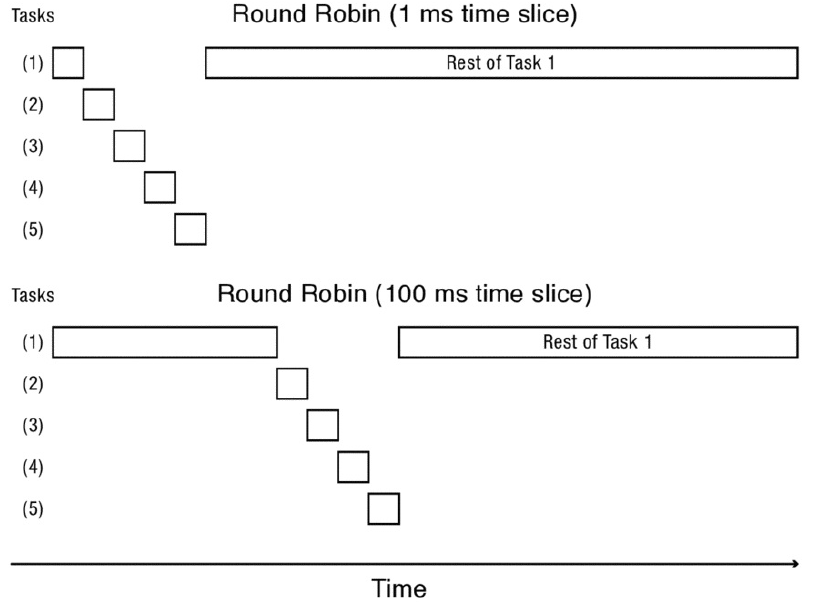
\includegraphics[scale=0.70]{img/fig0702}}
\caption{Tiempos de finalización con la programación Round Robin cuando llegan tareas cortas justo después de una tarea larga, con un tiempo de 1 ms (arriba) y 100 ms (abajo).}
\label{fig0702}
\end{figure}

Por supuesto, tenemos que escoger el quantum de tiempo cuidadosamente. Una consideración es de arriba: si tenemos un quantum de tiempo demasiado corto, el procesador pasará todo su tiempo cambiando y recibiendo muy poco trabajo útil. Si tomamos un tiempo demasiado largo, las tareas tendrán que esperar mucho tiempo hasta que tengan un turno. La Figura \ref{fig0702} muestra el comportamiento de Round Robin, en la misma carga de trabajo que en la Figura \ref{fig0701}, para dos valores diferentes para el quantum de tiempo.

Una forma de ver Round Robin es como un compromiso entre FIFO y SJF. En un extremo, si el quantum de tiempo es infinito (o al menos, más largo que la tarea más larga), Round Robin se comporta exactamente igual que FIFO. Cada tarea se ejecuta hasta su finalización y luego entrega el procesador al siguiente en línea. En el otro extremo, supongamos que fue posible cambiar entre tareas con cero sobrecarga, por lo que podríamos elegir un tiempo cuántico de una sola instrucción. Con el corte de tiempo de grano fino, las tareas terminarían en el orden de longitud, como con SJF, pero más lento: una tarea A se completará dentro de un factor de n de cuando tendría bajo SJF, donde n es el número máximo de tareas ejecutables.

\begin{figure}[tbhp]
\centerline{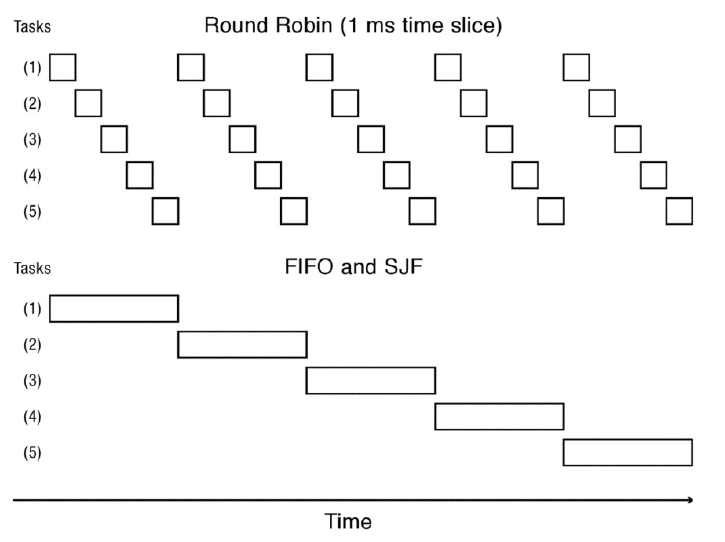
\includegraphics[scale=0.70]{img/fig0703}}
\caption{Tiempos de finalización con Round Robin (arriba) frente a FIFO y SJF (abajo) al programar tareas de igual longitud.}
\label{fig0703}
\end{figure}

Desafortunadamente, Round Robin tiene algunas debilidades. La Figura \ref{fig0703} ilustra lo que sucede para FIFO, SJF y Round Robin cuando varias tareas comienzan aproximadamente a la misma hora y son de la misma longitud. Round Robin girará a través de las tareas, haciendo un poco de cada una, terminando todas en aproximadamente el mismo tiempo. Esta es casi la peor política de programación posible para esta carga de trabajo. FIFO hace mucho mejor, escogiendo una tarea y pegándose con ella hasta que termine. No sólo FIFO reduce el tiempo de respuesta promedio para esta carga de trabajo en relación con Round Robin, ninguna tarea está peor con FIFO - cada tarea termina al menos tan pronto como lo haría en Round Robin. El cortar del tiempo agregó la sobrecarga sin ningún beneficio. Finalmente, considere lo que SJF hace en esta carga de trabajo. SJF programa tareas en exactamente el mismo orden que FIFO. La primera tarea que llegue se asignará al procesador, y tan pronto como ejecute una sola instrucción, tendrá menos tiempo restante que todas las otras tareas, y por lo tanto se ejecutará hasta su finalización. Dado que sabemos que SJF es óptimo para el tiempo de respuesta promedio, esto significa que tanto FIFO como Round Robin son óptimos para algunas cargas de trabajo y pesimales para otros, sólo diferentes en cada caso.

Dependiendo del quantum de tiempo, Round Robin también puede ser bastante pobre cuando se ejecuta una mezcla de tareas vinculadas a E/S y tareas de compilación. Las tareas de E/S suelen necesitar períodos muy cortos en el procesador para calcular la operación de E/S siguiente para emitir. Cualquier retraso que se programe en el procesador puede conducir a ralentizaciones en todo el sistema. Por ejemplo, en un editor de texto, a menudo toma sólo unos pocos milisegundos para hacer eco de una pulsación de tecla a la pantalla, un retraso mucho más rápido que la percepción humana. Sin embargo, si estamos compartiendo el procesador entre un editor de texto y varias otras tareas usando Round Robin, el editor debe esperar varios cuantos de tiempo para programar cada golpe de tecla - con un tiempo de $100 ms$, esto puede resultar molesto para el usuario.

\subsection{Max-Min Fairness - Equidad máxima-mínima}
En muchos entornos, una asignación justa de recursos es tan importante para el diseño de un programador como la capacidad de respuesta y la baja sobrecarga. En una máquina multiusuario o en un servidor, no queremos permitir que un solo usuario pueda monopolizar los recursos de la máquina, degradando el servicio para otros usuarios. Aunque puede parecer que la justicia tiene poco valor en las máquinas de un solo usuario, las aplicaciones individuales a menudo son escritas por diferentes compañías, cada una con un interés en hacer que el rendimiento de sus aplicaciones parezca bueno incluso si eso tiene un costo degradante para otras aplicaciones.

Otra complicación surge si debemos asignar recursos de manera justa entre usuarios, aplicaciones, procesos o subprocesos. Algunas aplicaciones pueden ejecutarse dentro de un solo proceso, mientras que otras pueden crear muchos procesos, y cada proceso puede implicar múltiples subprocesos. Round Robin entre los hilos puede conducir a la inanición si las aplicaciones con un solo hilo están compitiendo con las aplicaciones con cientos de hilos. Podemos preocuparnos por la asignación justa en cualquiera de estos niveles de granularidad: hilos dentro de un proceso, procesos para un usuario en particular, usuarios que comparten una máquina física. Por ejemplo, podríamos preocuparnos de asegurarnos de que cada hilo dentro de un proceso progrese. Sin embargo, para simplificar, nuestra discusión supondrá que estamos interesados en proporcionar equidad entre los procesos; los mismos principios se aplican si la unidad que recibe los recursos es el usuario, la aplicación o el hilo.

La equidad es fácil si todos los procesos están calculados: Round Robin dará a cada proceso una parte igual del procesador. En la práctica, sin embargo, diferentes procesos consumen recursos a diferentes ritmos. Un proceso vinculado a E/S puede necesitar sólo una pequeña parte del procesador, mientras que un proceso dependiente de computo está dispuesto a consumir todo el tiempo de procesador disponible. ¿Qué es una asignación equitativa cuando hay una diversidad de necesidades?

Una posible respuesta es decir que cualquier cosa que Round Robin hace es justo - después de todo, cada proceso tiene una oportunidad igual en el procesador. Sin embargo, como vimos anteriormente, Round Robin puede resultar en procesos de E/S que se ejecutan a una velocidad mucho más lenta de lo que lo harían si tuvieran el procesador para sí mismos, mientras que los procesos de computo limitado apenas se ven afectados. ¡Eso no parece justo!

Si bien hay muchas definiciones posibles de equidad, una particularmente útil se llama \textit{Max-Min Fairness}. Max-min imparcialidad iterativamente maximiza la asignación mínima asignada a un proceso particular (usuario, aplicación o hilo) hasta que se asignen todos los recursos. Si todos los procesos están calculados, el comportamiento de max-min es simple: maximizamos el mínimo dando a cada proceso exactamente la misma proporción del procesador, es decir, usando Round Robin.

El comportamiento de la igualdad max-min es más interesante si algunos procesos no pueden usar su parte entera, por ejemplo, porque son de ejecución corta o vinculados a E/S. Si es así, damos a esos procesos toda su solicitud y redistribuimos la parte no utilizada a los procesos restantes. Algunos de los procesos que reciben la porción adicional pueden no ser capaces de usar su totalidad de la parte revisada, por lo que debemos iterar, redistribuyendo cualquier parte no utilizada. Cuando no se satisfacen plenamente las solicitudes restantes, dividimos el resto de manera igual entre todos los procesos restantes.

Una implementación hipotética pero completamente impracticable de max-min sería dar al procesador en cada instante al procedimiento que haya recibido la menor parte del procesador. Sin embargo, ya hemos visto por qué esto no funcionaría bien. Con dos tareas igualmente largas, tan pronto como ejecutamos una instrucción en una tarea, habría recibido más recursos que la otra, por lo que para preservar la "equidad" necesitaríamos cambiar al instante a la siguiente tarea.

Podemos aproximar una asignación de la max-min justo al relajar esta restricción - para permitir que un proceso para adelantarse a su asignación equitativa en un tiempo cuántico. Cada vez que el programador necesita hacer una elección, elige la tarea para el proceso con el menor tiempo acumulado en el procesador. Si un nuevo proceso llega a la cola con mucho menos tiempo acumulado, como la tarea de disco, evitará el proceso, pero de lo contrario el proceso actual completará su quantum. Las tareas pueden llegar hasta una cantidad de tiempo más que su cuota justa, pero a largo plazo la asignación se igualará.

El algoritmo que acabamos de describir fue originalmente definido para la red, y no para el procesador, la planificación. Si compartimos un enlace entre una solicitud de navegador y una descarga larga, obtendremos una respuesta razonable para el navegador si tenemos una asignación justamente justa: el navegador necesita pocos paquetes de red y, por lo tanto, en max-min sus paquetes siempre se programarán antes de Los paquetes de la descarga.

Incluso esta aproximación, sin embargo, puede ser computacionalmente costosa, ya que requiere que las tareas se mantengan en una cola de prioridad. Para algunos entornos de servidor, puede haber decenas o incluso cientos de miles de decisiones de programación que deben hacerse cada segundo. Para reducir la sobrecarga computacional del planificador, la mayoría de los sistemas operativos comerciales utilizan un algoritmo algo diferente, con el mismo objetivo, que describiremos a continuación.

\subsection{Caso de Estudio: Multi-Level Feedback (Retroalimentación Multinivel)}
La mayoría de los sistemas operativos comerciales, incluyendo Windows, MacOS y Linux, usan un algoritmo de programación llamado cola de comentarios de nivel múltiple (MFQ). MFQ está diseñado para lograr varios objetivos simultáneos:
\begin{itemize}
\item \textbf{Sensibilidad}. Ejecutar tareas cortas rápidamente, como en SJF.
\item \textbf{Gastos indirectos bajos}. Minimizar el número de preemptions, como en FIFO, y minimizar el tiempo dedicado a tomar decisiones de planificación.
\item \textbf{Inanición-Libertad}. Todas las tareas deben progresar, como en Round Robin.
\item \textbf{Tarea en segundo plano}. Aplazar las tareas de mantenimiento del sistema, como la desfragmentación del disco, para que no interfieran con el trabajo del usuario.
\item \textbf{Justicia}. Asignar (no de fondo) procesa aproximadamente su participación justa mínima del procesador.
\end{itemize}

Al igual que con cualquier sistema real que debe equilibrar varios objetivos contradictorios, el MFQ no logra perfectamente ninguno de estos objetivos. Más bien, se pretende que sea un compromiso razonable en la mayoría de los casos del mundo real. MFQ es una extensión de Round Robin. En lugar de una sola cola, MFQ tiene varias colas Round Robin, cada una con un nivel de prioridad y un quantum de tiempo diferentes. Las tareas con un nivel de prioridad más alto prevén las tareas de menor prioridad, mientras que las tareas del mismo nivel están programadas en la forma de Round Robin. Además, los niveles de prioridad más altos tienen cuantos de tiempo más cortos que los niveles inferiores.

Las tareas se mueven entre los niveles de prioridad para favorecer las tareas cortas sobre las largas. Una nueva tarea entra en el nivel de prioridad superior. Cada vez que la tarea usa su quantum de tiempo, baja un nivel; Cada vez que la tarea rinde al procesador porque está esperando en la E/S, permanece en el mismo nivel (o se eleva un nivel); Y si la tarea se completa, sale del sistema.

Una nueva tarea de cálculo se iniciará como alta prioridad, pero rápidamente se agotará su cantidad de tiempo y caer a la próxima prioridad más baja, y luego la siguiente. Por lo tanto, una tarea de E/S que necesite sólo una cantidad modesta de computación casi siempre se programará rápidamente, manteniendo el disco ocupado. Las tareas relacionadas con el cálculo se ejecutan con una cantidad de tiempo prolongada para minimizar la sobrecarga de conmutación mientras se comparte el procesador.

Hasta ahora, el algoritmo que hemos descrito no alcanza la libertad de inanición ni la imparcialidad max-min. Si hay demasiadas tareas vinculadas a E/S, las tareas dependientes de computación pueden no recibir tiempo en el procesador. Para combatir esto, el planificador de MFQ monitorea cada proceso para asegurar que está recibiendo su parte justa de los recursos. En cada nivel, Linux realmente mantiene dos colas - tareas cuyos procesos ya han alcanzado su parte justa sólo están programadas si todos los demás procesos a ese nivel también han recibido su parte justa. Periódicamente, cualquier proceso que reciba menos que su cuota justa tendrá sus tareas aumentadas en prioridad; Igualmente, las tareas que reciben más que su parte justa se pueden reducir en prioridad.

El ajuste de la prioridad también aborda el comportamiento estratégico. Desde un punto de vista puramente egoísta, una tarea puede intentar mantener su prioridad alta haciendo una petición de E/S corta inmediatamente antes de que expire su tiempo cuántico. Eventualmente, el sistema detectará esto y reducirá su prioridad a su nivel de participación justa.

\subsection{Resumen}
\begin{itemize}
\item FIFO es simple y minimiza la sobrecarga.
\item Si las tareas son variables en tamaño, el FIFO puede tener un tiempo de respuesta promedio muy bajo.
\item Si las tareas son iguales en tamaño, FIFO es óptima en términos de tiempo de respuesta promedio.
\item Teniendo en cuenta sólo el procesador, SJF es óptimo en términos de tiempo de respuesta promedio.
\item SJF es pesimal en términos de variación en el tiempo de respuesta.
\item Si las tareas son de tamaño variable, Round Robin aproxima a SJF.
\item Si las tareas son iguales en tamaño, Round Robin tendrá un tiempo de respuesta promedio muy bajo.
\item Las tareas que mezclan el procesador y las E / S se benefician de SJF y pueden hacerlo mal bajo Round Robin.
\item La imparcialidad de Max-min puede mejorar el tiempo de respuesta para las tareas de E / S.
\item Round Robin y Max-min justness tanto evitar el hambre.
\item Mediante la manipulación de la asignación de tareas a las colas de prioridad, un planificador MFQ puede lograr un equilibrio entre la capacidad de respuesta, la sobrecarga baja y la imparcialidad.
\end{itemize}

\chapter{11 File Systems - Sistema de Archivos: Introducción y Visión General}
Los ordenadores deben poder almacenar de forma fiable los datos. Las personas almacenan fotos familiares, archivos de música y carpetas de correo electrónico. Los programadores almacenan documentos de diseño y archivos de origen. De hecho, para que una computadora trabaje en absoluto, necesita poder almacenar programas para funcionar y el sistema operativo, en sí mismo.

Para todos estos casos, los usuarios exigen mucho de sus sistemas de almacenamiento:
\begin{itemize}
\item \textbf{Confiabilidad}. Los datos de un usuario deben almacenarse de forma segura incluso si la máquina está apagada o su sistema operativo se bloquea. De hecho, gran parte de estos datos es tan importante que los usuarios esperan y necesitan los datos para sobrevivir incluso si los dispositivos utilizados para almacenarlos están dañados. Por ejemplo, muchos sistemas modernos de almacenamiento continúan funcionando incluso si uno de los discos magnéticos almacena el mal funcionamiento de datos o incluso si un centro de datos que aloja algunos de los servidores del sistema se quema.

\item \textbf{Gran capacidad y bajo costo}. Los usuarios y las empresas almacenan una enorme cantidad de datos, por lo que quieren poder comprar almacenamiento de alta capacidad por un bajo costo.

\item \textbf{Alto rendimiento}. Para que los programas utilicen datos, deben poder acceder a él, y para que los programas utilicen grandes cantidades de datos, este acceso debe ser rápido.

\item \textbf{Nombrar los Datos}. Debido a que los usuarios almacenan una gran cantidad de datos, debido a que algunos datos deben durar más tiempo que el proceso que lo crea, y porque los datos deben compartirse entre programas, los sistemas de almacenamiento deben proporcionar formas de identificar fácilmente los datos de interés. 

\item \textbf{Distribución controlada}. Los usuarios deben ser capaces de compartir datos almacenados, pero este intercambio debe ser controlado.
\end{itemize}

\textbf{Sistemas de almacenamiento y archivos no volátiles.}

El contenido de la memoria DRAM principal de un sistema se puede perder si se produce un fallo del sistema operativo o una falla de energía. Por el contrario, el almacenamiento no volátil es duradero y conserva su estado a través de choques y apagones; El almacenamiento no volátil también se llama almacenamiento persistente o almacenamiento estable. El almacenamiento no volátil también puede tener una capacidad mucho mayor y un costo menor que la DRAM volátil que forma la mayor parte de la mayoría de la memoria principal del sistema.

Sin embargo, las tecnologías de almacenamiento no volátil tienen sus propias limitaciones. Por ejemplo, las actuales tecnologías de almacenamiento no volátil, tales como discos magnéticos y almacenamiento flash de alta densidad, no permiten el acceso aleatorio a palabras individuales de almacenamiento; En su lugar, el acceso debe hacerse en unidades de grano más grueso - 512, 2048, o más bytes a la vez.

Además, estos accesos pueden ser mucho más lentos que el acceso a DRAM; Por ejemplo, la lectura de un sector de un disco magnético puede requerir la activación de un motor para mover un brazo de disco a una pista deseada en el disco y luego esperar a que el disco giratorio traiga los datos deseados debajo de la cabeza de disco. Debido a que los accesos de disco implican motores y movimiento físico, el tiempo para acceder a un sector aleatorio en un disco puede ser alrededor de $10$ milisegundos. Por el contrario, las latencias de DRAM suelen estar por debajo de $100$ nanosegundos. Esta gran diferencia - alrededor de cinco órdenes de magnitud en el caso de discos giratorios - impulsa al sistema operativo a organizar y utilizar dispositivos de almacenamiento persistente de manera diferente a la memoria principal.

Los sistemas de archivos son una abstracción común del sistema operativo para permitir que las aplicaciones accedan al almacenamiento no volátil. Los sistemas de archivos utilizan una serie de técnicas para hacer frente a las limitaciones físicas de los dispositivos de almacenamiento no volátil y para proporcionar mejores abstracciones a los usuarios.

\begin{itemize}
\item \textbf{Rendimiento}. Los sistemas de archivos amortizan el costo de iniciar operaciones costosas -como mover un brazo de disco o borrar un bloque de memoria de estado sólido- agrupando donde su ubicación de datos para que tales operaciones accedan a rangos de almacenamiento grandes y secuenciales.

\item \textbf{Nombres}. Los sistemas de archivos agrupan los datos relacionados en directorios y archivos y proporcionan nombres legibles para ellos (por ejemplo, /home/alice/Pictures/summer-vacation/hiking.jpg.) Estos nombres de datos siguen siendo significativos incluso después del programa que crea las salidas de datos, ayudan a los usuarios a organizar grandes cantidades de almacenamiento y facilitan a los usuarios el uso de diferentes programas para crear, leer y editar sus datos.

\item \textbf{Distribución controlada}. Los sistemas de archivos incluyen metadatos sobre quién posee qué archivos y qué otros usuarios pueden leer, escribir o ejecutar archivos de datos y programas.

\item \textbf{Confiabilidad}. Los sistemas de archivos utilizan transacciones para actualizar atómicamente varios bloques de almacenamiento persistente, similar a cómo el sistema operativo utiliza secciones críticas para actualizar atómicamente diferentes estructuras de datos en la memoria. Para mejorar aún más la confiabilidad, los sistemas de archivos almacenan sumas de comprobación con datos para detectar bloques dañados, y replican datos a través de múltiples dispositivos de almacenamiento para recuperarse de fallas de hardware.
\end{itemize}

\textbf{Impacto en los escritores de aplicaciones}.

Comprender las propiedades de fiabilidad y rendimiento del hardware de almacenamiento y de los sistemas de archivos es importante incluso si no está diseñando un sistema de archivos desde cero. Debido a las limitaciones fundamentales de los dispositivos de almacenamiento existentes, las ilusiones de nivel superior de fiabilidad y rendimiento proporcionadas por el sistema de archivos son imperfectas. Un programador de aplicaciones necesita comprender estas limitaciones para evitar tener datos inconsistentes almacenados en el disco o tener un programa ejecutando órdenes de magnitud más lentas de lo esperado.

Por ejemplo, supongamos que edita un documento grande con muchas imágenes incrustadas y que su procesador de textos guarda automáticamente el documento de forma que no pierda demasiadas ediciones si la máquina se bloquea. Si la aplicación utiliza el sistema de archivos de una manera sencilla, varias cosas inesperadas pueden ocurrir:

\begin{itemize}
\item \textbf{Bajo rendimiento}. En primer lugar, aunque los sistemas de archivos permiten que los bytes existentes en un archivo se sobrescriban con nuevos valores, no permiten que se inserten nuevos bytes en el medio de los bytes existentes. Por lo tanto, incluso una pequeña actualización del archivo puede requerir la reescritura de todo el archivo desde el principio hasta el final o al menos desde el punto de la primera inserción hasta el final. En el caso de un archivo de varios megabytes, cada autoguardado puede terminar tardando hasta un segundo.

\item \textbf{Archivo dañado}. En segundo lugar, si la aplicación simplemente sobrescribe el archivo existente con los datos actualizados, un accidente inoportuno puede dejar el archivo en un estado inconsistente, que contiene una mezcolanza de las versiones viejas y nuevas.

\item \textbf{Archivo perdido}. En tercer lugar, si en lugar de sobrescribir el archivo de documento, la aplicación escribe actualizaciones en un nuevo archivo, luego elimina el archivo original y finalmente mueve el nuevo archivo a la ubicación del archivo original, un accidente inoportuno puede dejar el sistema sin copias del documento en absoluto.
\end{itemize}

Los programas utilizan una variedad de técnicas para hacer frente a este tipo de problemas. Por ejemplo, algunos estructuran su código para aprovechar la semántica detallada de sistemas operativos específicos. Algunos sistemas operativos garantizan que cuando un archivo se cambia de nombre y ya existe un archivo con el nombre de destino, el nombre de destino siempre se referirá al archivo antiguo o nuevo, incluso después de un fallo en medio de la operación de cambio de nombre. En tal caso, una implementación puede crear un nuevo archivo con la nueva versión de los datos y usar el comando rename para sustituir atómicamente la versión anterior por la nueva.

Otros programas esencialmente construyen un sistema de archivos en miniatura sobre la parte superior del subyacente, estructurando sus datos para que el sistema de archivos subyacente pueda satisfacer mejor sus requisitos de rendimiento y confiabilidad.

\section{11.1 La abstracción del sistema de archivos}
Hoy en día, casi cualquier persona que utiliza una computadora está familiarizada con la abstracción del sistema de archivos de alto nivel. Los sistemas de archivos proporcionan a los usuarios una forma de organizar sus datos y almacenarlos durante largos períodos de tiempo.

Más precisamente, un sistema de archivos es una abstracción del sistema operativo que proporciona datos persistentes y nombrados. Los datos persistentes se almacenan hasta que se borran explícitamente, incluso si la computadora que lo almacena se bloquea o pierde energía. Se puede acceder a los datos nombrados a través de un identificador legible por humanos que el sistema de archivos asocia con el archivo. Tener un nombre permite que se acceda a un archivo incluso después de que el programa que lo creó ha salido y permite que sea compartido por múltiples aplicaciones.

Hay dos partes clave para la abstracción del sistema de archivos: archivos, que definen conjuntos de datos y directorios, que definen los nombres de los archivos.

\textbf{Archivo}. 

Un archivo es una colección con nombre de datos en un sistema de archivos. Por ejemplo: los programas \textit{/Aplicaciones} \textit{/Calculadora} o \textit{/ProgramFiles} \textit{/TextEdit} son archivos, al igual que los datos \textit{/home/Bob/correspondence/letter-to-mom.txt} o \textit{/home/Bob/Classes/OS/hw1.TXT}.

Los archivos proporcionan una abstracción de nivel más alto que el dispositivo de almacenamiento subyacente: permiten que un nombre único y significativo haga referencia a una cantidad de datos (casi) de tamaño arbitrario. Por ejemplo \textit{/home/Bob/Classes/OS/hw1.txt} puede almacenarse en el disco en los bloques $0x0A713F28$, $0xB3CA349A$ y $0x33A229B8$, pero es mucho más conveniente hacer referencia a los datos por su nombre que por esta lista de direcciones de disco.

La información de un archivo tiene dos partes, \textbf{metadatos} y \textbf{datos}. Los metadatos de un archivo son información sobre el archivo que el sistema operativo entiende y administra. Por ejemplo, los metadatos de un archivo suelen incluir el tamaño del archivo, su hora de modificación, su propietario y su información de seguridad, como si puede ser leída, escrita o ejecutada por el propietario o por otros usuarios.

Los datos de un archivo pueden ser cualquier información que un usuario o aplicación pone en él. Desde el punto de vista del sistema de archivos, los datos de un archivo son sólo una matriz de bytes no tipificados. Las aplicaciones pueden utilizar estos bytes para almacenar la información que quieran en cualquier formato que elijan. Algunos datos tienen una estructura simple. Por ejemplo, un archivo de texto ASCII contiene una secuencia de bytes que se interpretan como letras en el alfabeto inglés. Por el contrario, las estructuras de datos almacenadas por las aplicaciones pueden ser arbitrariamente complejas. Por ejemplo, los archivos $.doc$ pueden contener texto, información de formato y objetos e imágenes incrustados, los archivos $ELF$ (archivo ejecutable y vinculable) pueden contener objetos compilados y código ejecutable o un archivo de base de datos puede contener la información y los índices administrados por un base de datos relacional.

\textbf{Directorio}. 

Mientras que un archivo contiene metadatos definidos por el sistema y datos arbitrarios, los directorios proporcionan nombres para los archivos. En particular, un directorio de archivos es una lista de nombres legible por humanos y una correspondencia de cada nombre de un archivo o directorio subyacente específica. Una metáfora común es que un directorio es una carpeta que contiene documentos (archivos) y otras carpetas (directorios).

Debido a que los directorios pueden incluir nombres de otros directorios, pueden organizarse en una jerarquía para que se puedan agrupar diferentes conjuntos de archivos asociados en directorios diferentes. Por lo tanto, el directorio \textit{/bin} puede incluir aplicaciones binarias para su máquina mientras que \textit{/home/tom} (el "directorio personal" de Tom) podría incluir archivos de Tom. Si Tom tiene muchos archivos, su directorio puede incluir directorios adicionales para agruparlos (por ejemplo, \textit{/home/tom/Music} y \textit{/home/tom/Work}.) Cada uno de estos directorios puede tener subdirectorios (por ejemplo, \textit{/home/tom/Work/Class} y \textit{/home/tom/Work/Docs}) y así sucesivamente.

La cadena que identifica un archivo o directorio (por ejemplo, \textit{/home/tom/Work/Class/OS/hw1.txt}) se denomina \textbf{ruta}. Aquí, el símbolo $/$ (barra pronunciada) separa componentes de la ruta, y cada componente representa una entrada en un directorio. Por lo tanto, \textit{hw1.txt} es un archivo en el directorio OS; OS es un directorio en el directorio Trabajo; y así.

Si piensa en el directorio como un árbol, entonces la raíz del árbol es un directorio llamado, naturalmente, el directorio raíz. Nombres de ruta como \textit{/bin/ls} que comienzan con $/$ definen rutas absolutas que se interpretan en relación con el directorio raíz. Por lo tanto, \textit{/home} se refiere al directorio llamado \textit{home} en el directorio raíz.

Los nombres de ruta como \textit{Work/Class/OS} que no comienzan con $/$ definen rutas de acceso relativas interpretadas por el sistema operativo en relación con el directorio de trabajo actual de un proceso. Por lo tanto, si el directorio de trabajo actual de un proceso es \textit{/home/tom}, entonces la ruta relativa \textit{Work/Class/OS} es equivalente a la ruta absoluta \textit{/home/tom/Work/ Class/OS}.

Cuando inicia sesión, el directorio de trabajo actual de su \textit{shell} está configurado en su directorio personal. Los procesos pueden cambiar su directorio de trabajo actual con la llamada al sistema \textit{chdir} (ruta). Por ejemplo, si inicia sesión y, a continuación, escribe \textit{cd Work/Class/OS}, su directorio de trabajo actual se cambia desde su directorio principal al subdirectorio \textit{Work/Class/OS} en su directorio personal.

La asignación entre un nombre y el archivo subyacente se denomina enlace duro. Si un sistema de sistema permite múltiples enlaces duros al mismo archivo, entonces la jerarquía de directorios ya no puede ser un árbol. La mayoría de los sistemas de archivos que permiten múltiples enlaces duros a un archivo restringen estos enlaces para evitar ciclos, asegurando que sus estructuras de directorio forman un grafo acíclico dirigido (DAG). Evitar ciclos puede simplificar la administración, por ejemplo, asegurando que los recorridos recursivos de una estructura de directorio Terminar o haciendo fácil recurrir al recuento de referencias para recolectar un archivo cuando se elimine el último enlace a él.

\textbf{Volumen}. 

Cada instancia de un sistema de archivos administra archivos y directorios para un volumen. Un volumen es una colección de recursos físicos de almacenamiento que forman un dispositivo de almacenamiento lógico.

Un volumen es una abstracción que corresponde a un disco lógico. En el caso más simple, un volumen corresponde a una sola unidad de disco físico. Alternativamente, se puede particionar un solo disco físico y almacenar varios volúmenes o varios discos físicos se pueden combinar de manera que un solo volumen abarque varios discos físicos.

Un único equipo puede utilizar varios sistemas de archivos almacenados en varios volúmenes al montar varios volúmenes en una única jerarquía lógica. El montaje de un volumen en un sistema de archivos existente crea una asignación desde una ruta en el sistema de archivos existente al directorio raíz del sistema de archivos del volumen montado y permite que las asignaciones de control de sistema de archivos montadas para todas las extensiones de esa ruta.


\begin{figure}[tbhp]
\centerline{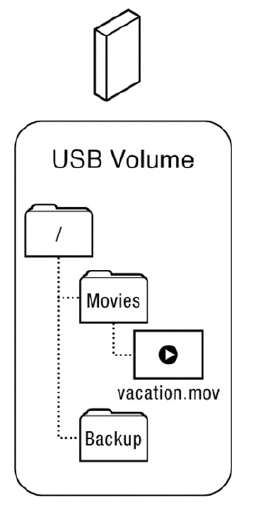
\includegraphics[scale=0.70]{img/fig1101}}
\caption{Este disco USB contiene un volumen que es el almacenamiento físico para un sistema de archivos.}
\label{fig1101}
\end{figure}

\begin{figure}[tbhp]
\centerline{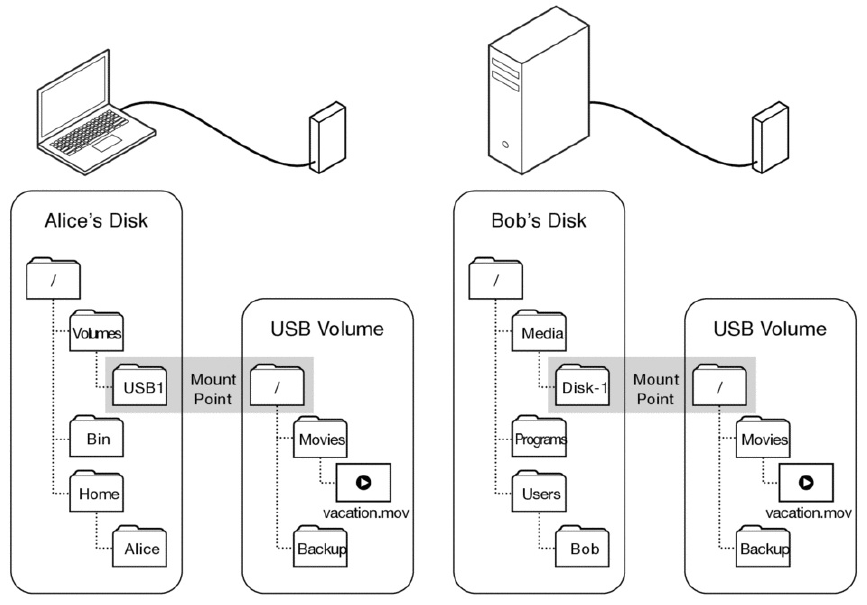
\includegraphics[scale=0.70]{img/fig1102}}
\caption{Un volumen puede montarse en otro sistema de archivos para unirse a sus jerarquías de directorios. Por ejemplo, cuando la unidad USB está conectada al ordenador de Alice, puede acceder a la película vacation.mov usando la ruta /Volumes/usb1/Movies/vacation.mov y cuando la unidad está conectada al ordenador de Bob, puede acceder a la película Utilizando la ruta /media/disk-1/Movies/vacation.mov.}
\label{fig1102}
\end{figure}

Por ejemplo, suponga que una unidad USB contiene un sistema de archivos con los directorios \textit{/Películas} y \textit{/Backup} como se muestra en la Figura \ref{fig1101}. Si Alice conecta esa unidad en su computadora portátil, el sistema operativo del portátil podría montar el sistema de archivos del volumen USB con la ruta \textit{/Volúmenes/usb1/} como se muestra en la Figura \ref{fig1102}. Luego, si Alice llama abierta \textit{/Volumes/usb1/Movies/vacation.mov}, abrirá el archivo \textit{/Movies/vacation.mov} del sistema de archivos en el volumen de la unidad USB. Si, en cambio, Bob se conecta a su computadora portátil, el sistema operativo del portátil podría montar el sistema de archivos del volumen con la ruta \textit{/media/disk-1}, y Bob accedería al mismo archivo usando la ruta \textit{/media/disk-1/Películas/Vacation.mov}.


\section{11.2 API}
\textbf{Creación y Eliminación de Archivos y Directorios.}

Los procesos crean y destruyen archivos con \textit{create()} y \textit{unlink()}. Create() hace dos cosas: crea un archivo nuevo que tiene metadatos iniciales pero no otros datos y crea un nombre para ese archivo en un directorio.

\textit{Link()} crea un vínculo duro: un nuevo nombre de ruta para un archivo existente. Después de una llamada exitosa a \textit{link()}, hay varios nombres de ruta que se refieren al mismo archivo subyacente.

\textit{Unlink()} elimina un nombre para un archivo de su directorio. Si un archivo tiene varios nombres o vínculos, \textit{unlink()} sólo elimina el nombre especificado, dejando el archivo accesible a través de otros nombres. Si el nombre especificado es el último (o único) vínculo a un archivo, entonces \textit{unlink()} también elimina el archivo subyacente y libera sus recursos.

\textit{Mkdir()} y \textit{rmdir()} crean y eliminan directorios.

\textbf{Abrir y Cerrar.}

Para iniciar el acceso a un archivo, un proceso llama a \textit{open()} para obtener un descriptor de archivo que puede usar para referirse al archivo abierto. El descriptor de archivo es terminología de Unix; En otros sistemas el descriptor puede llamarse un identificador de archivo o un flujo de archivo.

Los sistemas operativos requieren procesos para abrir explícitamente los archivos y acceder a ellos a través de descriptores de archivos en lugar de simplemente pasar el nombre de la ruta de acceso a las llamadas \textit{read()} y \textit{write()} por dos razones. En primer lugar, el análisis de ruta y la comprobación de permisos pueden realizarse justo cuando se abre un archivo y no es necesario repetirlo en cada lectura o escritura. En segundo lugar, cuando un proceso abre un archivo, el sistema operativo crea una estructura de datos que almacena información sobre el archivo abierto del proceso, como el ID del archivo, si el proceso puede escribir o simplemente leer el archivo y un puntero a la posición actual del proceso dentro de el archivo. El descriptor de archivo puede considerarse así como una referencia a la estructura de datos del sistema operativo por archivo abierto que el sistema operativo utilizará para administrar el acceso del proceso al archivo.

Cuando una aplicación se realiza mediante un archivo, llama a \textit{close()}, que libera el registro de archivo abierto en el sistema operativo.

\textbf{Acceso a Archivos.}

Mientras un archivo está abierto, una aplicación puede acceder a los datos del archivo de dos maneras. En primer lugar, puede utilizar la interfaz de procedimiento tradicional, haciendo llamadas de sistema a \textit{read()} y \textit{write()} en un archivo abierto. Las llamadas a \textit{read()} y \textit{write()} comienzan desde la posición actual del archivo del proceso, y avanzan la posición del archivo actual por el número de bytes que se han leído o escrito correctamente. Por lo tanto, una secuencia de las llamadas \textit{read()} o \textit{write()} se mueve secuencialmente a través de un archivo. Para admitir acceso aleatorio dentro de un archivo, la llamada \textit{seek()} cambia la posición actual de un proceso para un archivo abierto especificado.

En lugar de usar \textit{read()} y \textit{write()} para acceder a los datos de un archivo, una aplicación puede usar \textit{mmap()} para establecer una correlación entre una región de la memoria virtual del proceso y alguna región del archivo. Una vez que se ha asignado un archivo, la memoria carga y almacena en esa región de memoria virtual leerá y escribirá los datos del archivo, ya sea accediendo a una página compartida desde la caché de archivos del kernel o activando una excepción de fallo de página que haga que el kernel busque el archivo deseado Página de datos del sistema de archivos en la memoria. Cuando una aplicación se realiza con un archivo, puede llamar a \textit{munmap()} para eliminar las asignaciones.

Por último, la llamada \textit{fsync()} es importante para la confiabilidad. Cuando una aplicación actualiza un archivo a través de \textit{write()} o un almacén de memoria en un archivo asignado, las actualizaciones se guardan en memoria intermedia y se guardan en un almacenamiento estable en un futuro. \textit{Fsync()} garantiza que todas las actualizaciones pendientes de un archivo se escriban en almacenamiento persistente antes de que se devuelva la llamada. Las aplicaciones utilizan esta función para dos propósitos. En primer lugar, llamar a \textit{fsync()} asegura que las actualizaciones sean duraderas y no se perderán si hay un fallo o un fallo de energía. En segundo lugar, llamar a \textit{fsync()} entre dos actualizaciones asegura que la primera se escribe en el almacenamiento persistente antes de la segunda. Tenga en cuenta que llamar a \textit{fsync()} no siempre es necesario; El sistema operativo garantiza que todas las actualizaciones se hagan duraderas al limpiar periódicamente todos los bloques de archivos sucios a un almacenamiento estable.
%------------------------------------------------------------------------------------------------------------------------------------------
%	BIBLIOGRAFÍA
%------------------------------------------------------------------------------------------------------------------------------------------
\nocite{*}
\bibliographystyle{resumen}
\bibliography{resumen}


\end{document}